% !TEX encoding = ISO-8859-16
\documentclass[twocolumn]{svjour3}

% Be sure to use PDF Latex, important for arxiv
\pdfoutput=1

%% JMIV Specific %%
\smartqed  % flush right qed marks, e.g. at end of proof

\usepackage[latin1]{inputenc}
% \usepackage{amsmath,amssymb} % amsthm
\usepackage{graphicx}
%\usepackage{pdfsync}
\usepackage{epsfig}
\usepackage{epstopdf}
\usepackage{mystyle,ulem}
\usepackage{color}
\usepackage{microtype}
\usepackage{multirow}
\usepackage{url}
%
\graphicspath{{./img/}}
 % use Times fonts if available on your TeX system
\usepackage{mathptmx}




\title{Sliced and Radon Wasserstein Barycenters of Measures}

\author{
	Nicolas Bonneel \and Julien Rabin \and Gabriel Peyr\'e \and Hanspeter Pfister
}
%\authorrunning{Short form of author list} % if too long for running head

\institute{N. Bonneel \at
			  Harvard University and LIRIS-CNRS\\
              \email{nicolas.bonneel@liris.cnrs.fr}           
           	\and
           	J. Rabin \at
           	GREYC, Universit\'{e} de Caen and CNRS
		   \and G. Peyr\'{e} \at
		   CNRS and CEREMADE, Universit\'{e} Paris-Dauphine
		   \and H. Pfister \at
		   Harvard University
}

\setlength{\abovecaptionskip}{0.1cm plus2mm minus1mm}  %I'm not sure the editor will appreciate ; let's see. 
\setlength{\belowcaptionskip}{0.3cm plus2mm minus1mm}  %I'm not sure the editor will appreciate ; let's see. (no spacing after caption is rather ugly though)
\setlength{\floatsep}{0.3cm plus2mm minus1mm}
\setlength{\textfloatsep}{0.3cm plus2mm minus1mm}
\setlength{\dbltextfloatsep}{0.3cm plus2mm minus1mm}
\setlength{\dblfloatsep}{0.3cm plus2mm minus1mm}

%%%%%%%%%%%%%%%%%%%%%%%%%%%%%%%%%%%%%%%%%%%%%%%%%%%%%%%%%%%%%%%%
\begin{document}

\maketitle


\begin{abstract}
	This article details two approaches to compute barycenters of measures using {1-D} Wasserstein distances along radial projections of the input measures. The first me\-thod makes use of the Radon transform of the measures, and the second is the solution of a convex optimization problem over the space of measures. We show several properties of these barycenters and explain their relationship. We show numerical approximation schemes based on a discrete Radon transform and on the resolution of a non-convex optimization problem. We explore the respective merits and drawbacks of each approach on applications to two image processing problems: color transfer and texture mixing.   
\keywords{Optimal transport \and Radon transform \and Wasserstein distance \and Barycenter of measures}
\end{abstract}

%\newpage\quad \newpage\input{sections/sec-appendix}\newpage
% !TEX encoding = ISO-8859-16
\section{Introduction}

The mass transportation problem corresponds to the computation of an optimal warping to map (i.e. push-forward) a given input probability measure $\mu_0$ to a second probability measure $\mu_1$. The optimality corresponds to minimizing a cost (the so-called Wasserstein distance) associated to the warping, which measures the effort needed to perform the corresponding motion. Informally, the effort is expressed as the cost it would require to move a pile of sand representing $\mu_0$ toward a hole made of $\mu_1$, by summing the cost (typically a squared distance) for each particle of sand to reach its destination in the hole (see Fig.~\ref{fig:monge}).  We refer to~\cite{Villani03} for a review of the mathematical foundations of optimal transport. 

As a byproduct of the computation of this optimal transport, it is possible to define a geodesic $\mu_t$, for $t \in [0, 1]$ interpolating between the two input measures. This corresponds to the so-called displacement interpolation introduced by McCann~\cite{mccann1997convexity}. Such an interpolation has several  applications ranging from the analysis of PDEs to computer graphics, which we review below. Moreover, as introduced in~\cite{Carlier_wasserstein_barycenter}, this interpolation between two densities can be extended to an arbitrary number of measures by defining a barycenter according to the transportation distance. However, a major bottleneck is the computational complexity of computing the optimal transport, geodesics and barycenters in arbitrary dimension.  In this paper, we address these issues by leveraging the fact that these problems are easy to solve for 1-D distributions. We propose alternative definitions of barycenters using two frameworks based on 1-D projections of the measures. We describe the associated fast computational schemes, and show some applications in image processing (color transfer) and computer graphics (texture mixing).


% The mass transportation problem leads to an interpolation $\mu_t$ ($t \in [0, 1]$), called \textit{displacement interpolation}, that consists  in moving the probability measure $\mu_0$ partway toward $\mu_1$. This has shown to have a wide range of applications, from computer graphics~\cite{Bonneel-displacement,Rabin_ssvm11,matusik2005texture} to image processing~\cite{pitie2005n,haker2004}, due to the characteristic advection produced during the interpolation. While this interpolation can be very efficiently performed in one dimension, extending it to multiple dimensions is much more challenging and leads to computationally expensive solutions. In addition, further extending  the approach to an interpolation between more than two probability measures currently remains untractable. In this paper, we address both scalability and multi-marginal mass transportation through an approximate framework based on 1d projections. We present both a fast Eulerian approach and a more general Lagrangian approach, and analyze some properties they share.

\vspace{0.3cm}
\begin{figure}[!t]
\begin{center}
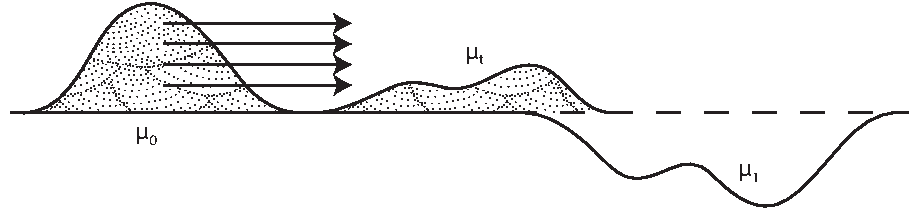
\includegraphics[width=\linewidth]{img/monge.pdf}
\end{center}
\caption{The mass transportation problem consists in optimally moving a probability measure $\mu_0$ represented by a pile of sand, toward a probability measure $\mu_1$ making a hole. At an intermediate time $t \in [0,1]$, an interpolated probability measure $\mu_t$, the \textit{displacement interpolation}, is obtained. A \textit{Wasserstein barycenter} generalizes this notion by considering more than $2$ probability measures.}
\label{fig:monge}
\end{figure}


%%%%%%%%%%%%%%%%%%%%%%%%%%%%%%%%%%%%%%%
\subsection{Previous work}

%%%
\paragraph{Computational Optimal transport.}

There is a vast literature on the numerical computation and approximation of the optimal transport plan. For discrete measures ({i.e.} sums of Dir\-acs), it boils down to the solution of a linear program, as initiated by Kantorovitch~\cite{Kantorovich42} which laid the modern foundations of transportation theory. There exist dedicated combinatorial optimization methods, such as the auction algorithm~\cite{Bertsekas1988} and the Hungarian algorithm~\cite{Kuhn-hungarian}. The $L^2$ optimal transport map is the solution of the celebrated Monge-Amp\`ere non-linear PDE. A variety of methods have been proposed to approximate numerically the solution to this equation, see for instance~\cite{Benamou2012} and references therein. 

% The optimization re\-qui\-red to compute the \textit{transport plan} -- the map that describes the motion of the probability measures -- can be performed in several ways. For instance, Bonneel et al. used a linear program with radial basis functions~\cite{Bonneel-displacement}. Benamou and Brenier exploited a fluid dynamic interpretation~\shortcite{Benamou2000}  which requires solving for a space-time Laplace equation, that Papadakis et al. efficiently performed via proximal splitting~\cite{FPapPeyOud13}. Haker et al. used Brenier's polar factorization to build a curl-free velocity field solving the transportation problem~\cite{haker2004}.  M�rigot proposed a multiscale geometric method based on power diagrams~\cite{Merigot2011} by computing the transport plan between diracs and a smooth density. These approaches however remain complex, and limited to the interpolation between two probability measures. 


%%%
\paragraph{Wasserstein geodesics. }

The Wasserstein geodesic (i.e. a minimizing length path interpolating between two measures) is easily computed by linearly interpolating between the identity and the optimal transport. It is thus a trivial by-product of the computation of the optimal map. Let us however notice that the landmark paper of Benamou and Brenier~\cite{Benamou2000} proposes to actually proceed the other way around, i.e., to compute the geodesic as the solution of a convex optimization problem. The drawback of this approach is that it requires the addition of an extra dimension (time parameterizing the geodesic), but it allows the computation of an accurate approximation of the geodesic on a fixed discretization grid. This algorithm has recently been revisited using proximal splitting optimization schemes~\cite{FPapPeyOud13} ; we make use of this approach to compare the Wasserstein geodesics with the one obtained through our methods. 

%%%
\paragraph{Wasserstein barycenters. }

Wasserstein barycenters generalize the notion of geodesic interpolation from two to an arbitrary number of measures. The mathematical foundation for the formulation of these barycenters (i.e. existence, uniqueness and linear programming formulation) is detailed in~\cite{Carlier_wasserstein_barycenter}. These barycenters have found application, for instance, in statistical estimation~\cite{BigotBarycenter}. They enjoy an almost closed form expression in the case of Gaussian measures. This property is used in~\cite{peyre2013Gaussians} to perform texture mixing of Gaussian texture models. 

Cuturi and Doucet propose in~\cite{CuturiBarycenter} a numerical scheme to approximate the Wasserstein barycenter on an Eulerian grid. They smooth the Wasserstein distance using an entropic penalization, allowing them to perform a gradient descent. To reduce the numerical complexity of the barycenter computation, Rabin et al.~\cite{Rabin_ssvm11} introduce a different variational problem that sums the Wasserstein distances of 1-D projections of the input measures. Our method generalizes the iterative 1-D histogram matching used in~\shortcite{pitie2005n} to alter color palettes. Our work builds on the initial construction of  Rabin et al.~\cite{Rabin_ssvm11}. We propose a more formal exposition of this method and its main properties, and also present an alternative formulation based on the Radon transform. 



%%%
\paragraph{Applications in imaging. }

There are numerous applications of mass transportation in image processing, computer vision and computer graphics. The Wasserstein distance leads to state-of-the-art results for several image retrieval problems, see for instance~\cite{Rubner1998} for an early work on this topic. The optimal transport plan has been used for color transfer in images~\cite{pitie2005n} and for meshing in computer graphics~\cite{digne-reconstruction}.  Displacement interpolation has been employed for image warping and registration~\cite{haker2004,Merigot2011}, to remove flickering in old movies~\cite{Delon-midway} and in computer graphics to perform manipulations on textures~\cite{matusik2005texture} and to interpolate reflectance for 3-D rendering~\cite{Bonneel-displacement}. The Wasserstein barycenter of Gaussian distributions has found applications for texture synthesis and mixing, using either non-parametric density estimations~\cite{Rabin_ssvm11} and Gaussian density estimation~\cite{peyre2013Gaussians}.


%%%%%%%%%%%%%%%%%%%%%%%%%%%%%%%%%%%%%%%%%%%%%%%%%%%%%%%%%%%%%%%%
\subsection{Contributions}

In this paper, we introduce two efficient methods to approximate the Wasserstein barycenter of an arbitrary number of measures based on 1-D projections. The first approach, that we call ``Radon barycenter'', computes 1-D barycenters of Radon projections of the input measures, and defines the resulting barycenter as a back-projection of these 1-D barycenters. This method leads to a fast numerical scheme for an Eulerian discretization of the measures (i.e. based on histograms on a regular lattice), using a discrete Radon transform.  The second approach, that we call ``sliced barycenter'', is defined as the solution of an optimization problem which integrates the distances of all the Radon projections. A Lagrangian discretization (i.e. using point clouds with freely moving positions) is well adapted to the numerical resolution of a non-convex re-formulation of this optimization problem. 

We demonstrate properties of these two barycenters, analyze their relationship and show how they compare in practice. We show that both approximations solve a similar variational problem that only differs in the lack of surjectivity of the Radon transform. We also prove that both barycenters exhibit similar translational and scaling properties as the exact Wasserstein barycenter at a fraction of its computational cost. We compare our approximation with  the exact barycenter of two probability measures using a state of the art method~\cite{FPapPeyOud13}. We exemplify typical usages of these two complementary approaches to solve a problem of color harmonization in image processing, and a problem of texture mixing in computer graphics. 

The code to reproduce the figure of this article is available online\footnote{\url{https://github.com/gpeyre/2014-JMIV-SlicedTransport}}.


%%%%%%%%%%%%%%%%%%%%%%%%%%%%%%%%%%%%%%%%%%%%%%%%%%%%%%%%%%%%%%%%
\subsection{Notations}

We denote $\SS^{d-1}$ the unit sphere in $\RR^d$, and we define $\Om^d = \RR \times \SS^{d-1}$. 
We denote $\d \th$ the uniform measure on the sphere, which is normalized to satisfy $\int_{\Sph} \d\th=1$. We write $\Cont{X}$ the space of continuous functions on $X$ tending to 0 at infinity, where in the following $X$ is either $\RR^d$ or $\Om^d$. It is a Banach space with respect to the norm 
\eq{
	\foralls f \in \Cont{X}, \quad \normi{f}=\umax{x \in X} |f(x)|.
} 
We denote as $\Mm(X)$ the Radon measures on $X$, which is the space of finite Borel measures on $X$, and can also be represented as the dual of $\Cont{X}$, i.e., it is the space of continuous linear forms on $\Cont{X}$. We write 
\eq{
	\foralls (\mu,g) \in \Mm(X) \times \Cont{X}, \quad 
		\int_X g(x) \d \mu(x) \in \RR
}
the duality pairing between these spaces, which evaluates at $g$ the linear form defined by $\mu$. $\Mm(X)$ is a Banach space with respect to the dual norm, which is the so-called total variation norm, $\foralls \mu \in \Mm(X)$
\eql{\label{eq-tv-norm}
	\norm{\mu}_{\text{TV}} = \max \enscond{ \int_X g(x) \d \mu(x) }{ g \in \Cont{X}, \; \normi{g} \leq 1 }.
}
In the following, the convex cone of positive Radon measures is written 
\eq{
	\Mm^+(X) = \enscond{ \mu }{ \foralls f \in \Cont{\RR^d}, f \geq 0, \: \int f \d\mu \geq 0 }.
} 

We denote as $\sharp$ the push-forward operator, which, for any measurable map $M : X \rightarrow Y$ defines a linear operator $M\sharp : \Mm(X) \rightarrow \Mm(Y)$ as, for any $\mu \in \Mm(X)$  
\eq{
	\foralls g \in \Cont{Y}, \quad
	\int_Y g(y) \d(M \sharp \mu)(y) = 
	\int_X g(M(x)) \d\mu(x).
}
If $\d\mu(x) = \rho(x)\d x$ has a density $\rho$ with respect to some measure $\d x$ (e.g., the Lebesgue measure on $\RR^d$), and if $M$ is a $C^1$ diffeomorphism, then one has
\eql{\label{eq-pushfwd-density}
	\d (M \sharp \mu)(y) = (\rho \circ M^{-1})(y) |\det(\partial M^{-1}(y))| \d y.
}

Using the disintegration theorem (see for instance~\cite{DellacherieBook}), one can slice a measure $\nu \in \Mm(\Om^d)$ into its conditional measures with respect to the uniform measure on $\SS^{d-1}$ to obtain a measure $\nu^\th \in \Mm(\RR)$ for almost all $\th \in \SS^{d-1}$ outside a Borel set of zero measure, which satisfies, $\foralls g \in \Cont{\Om^d}$
\eql{\label{eq-desintegration}
	\int_{\Om^d} g(t,\th) \d \nu(t,\th) = 
	\int_{\SS^{d-1}} \pa{ \int_\RR g(t,\th) \d\nu^\th(t)  } \d \th,
}
and such that for any Borel set $A \subset \RR$, $\th \in \SS^{d-1} \mapsto \nu^\th(A) \in \RR$ is a Borel map. 

The convex set of normalized positive probability measures is $\Mm_1^+(\RR^d) \subset \Mm^+(\RR^d)$, which are measures $\mu \in \Mm^+(\RR^d)$ which satisfy $\mu(\RR^d)=1$.
We also denote $\bar\Mm_1^+(\Om^d)$ the set of positive probability measures having normalized conditional mesures along the $t$ variable, i.e.,
\eq{
	\bar\Mm_1^+(\Om^d) = \enscond{ \nu \in \Mm_1^+(\Om^d) }{ \foralls \th \in \SS^{d-1}, \quad \nu^\th(\RR) = 1 }
}
where $\nu^\th \in \Mm_1^+( \RR )$ is the conditional measure defined according to the disintegration formula~\eqref{eq-desintegration}. 

We denote as $\de_x \in \Mm_1^+(\RR^d)$ the Dirac measure at $x \in \RR^d$, i.e. 
\eq{
	\foralls f \in \Cont{\RR^d}, \quad
		\int_{\RR^d} f(y) \d (\de_x)(y) = f(x).  
}

We write $\Dd(X)$ the space of $\Cc^\infty(X)$ functions with compact support, and $\Dd^*(X)$ its dual, which is the space of distributions.  

% We write $H^s(X)$ the Sobolev space of order $s$, which is the set of $f \in \Dd^*(X)$ such that $f^{(s)} \in \Ldeux(X)$ (possibly interpreted as a fractional derivative if $s$ is not integer). One has $\Mm(X) \subset H^s(X) \subset \Dd^*(X)$ for any $s<-d/2$ \todo{negative $d/2$? sure ?}.


The Fourier transform of $f \in \Lun(\RR^d)$ is defined as
\eq{
	\foralls \om \in \RR^d, \quad \hat f(\om) = \int_{\RR^d} f(x) e^{-\imath \dotp{\om}{x}} \d x,
}
and the Fourier transform of a measure $\mu \in \Mm(\RR^d)$ as
\eq{
	\foralls \om \in \RR^d, \quad \hat \mu(\om) = \int_{\RR^d} e^{-\imath \dotp{\om}{x}} \d \mu(x).
}

Given a finite index set $I$, we define the simplex set of weights as 
\eql{\label{eq-defn-simplex}
	\La_I = \enscond{ \la = (\la_i)_{i \in I} \in \RR^I }{ \foralls i \in I, \: \la_i \geq 0, \; \sum_{i \in I} \la_i = 1 }
}
where the notation $\RR^I$ corresponds to the set of vectors indexed by $I$. 
%For $\la \in \La_I$, we also define the mapping
%\eq{ 
%	\be_\la : x = (x_i)_{i \in I} \in  (\RR^d)^I \mapsto \sum_{i \in I} \la_i x_i \in \RR^d.
%}

We define the following translation and scaling operators, for all $(s,u) \in \RR^{+,*} \times \RR^d$, 
\begin{align*}
		\foralls x \in \RR^d, \quad
			\phi_{s,u}(x) &= s x + u \in \RR^d, \\ 
		\foralls (t,\th) \in \Om^d, \quad
			\psi_{s,u}(t, \th) &= (st+\dotp{u}{\th}, \th) \in \Om^d.
\end{align*}
We denote $\Oo(\RR^d)$ the orthogonal group of $\RR^d$, i.e. $\Phi : \RR^d \mapsto \RR^d$ is an invertible linear map with $\Phi^* = \Phi^{-1}$ the adjoint operator. For all $\Phi \in \Oo(\RR^d)$ we denote  
\eq{
	\tilde \Phi : (t,\th) \in \Om^d \mapsto (t,\Phi^* \th) \in \Om^d.
}
A measure $\mu$ is said to be radial (denoted $\mu \in \Rad(\RR^d)$) if $\Phi \sharp \mu = \mu$ for all rotation $\Phi \in \Oo(\RR^d)$. 
It is said to be centrally symmetric (denoted $\mu \in \Cent(\RR^d)$) if $S \sharp \mu = \mu$ for the central symmetry $S \in \Oo(\RR^d)$ such that $S = -\Id_{\RR^d}$. 

% !TEX encoding = ISO-8859-16
%%%%%%%%%%%%%%%%%%%%%%%%%%%%%%%%%%%%%%%%%%%%%%%%%%%%%%%%%%%%%%
%%%%%%%%%%%%%%%%%%%%%%%%%%%%%%%%%%%%%%%%%%%%%%%%%%%%%%%%%%%%%%%%
\section{Wasserstein Distance}
\label{sec-bary-wass}


%%
\subsection{Optimal Transport}

For $(\mu_1,\mu_2) \in \Mm_1^+(\RR^d)^2$, we define the $L^2$-Wasserstein distance $\Wass{\RR^d}(\mu_1,\mu_2)^2$ to be equal to
\eql{\label{eq-dfn-wass-dist}
	\inf \enscond{ 
		\int_{\RR^d \times \RR^d} \norm{x_1-x_2}^2 \d\ga(x_1,x_2)
	}{
		{ \ga \in C(\mu_1,\mu_2) }
	}
}
where 
\eq{
	C(\mu_1,\mu_2) = \enscond{ \ga \in \Mm_1^+(\RR^d \times \RR^d) }{ \Pi_i \sharp \ga = \mu_i, \;  i=1,2 }
}
where $\Pi_1(x_1,x_2) = x_1$ and $\Pi_2(x_1,x_2)=x_2$. We refer to~\cite{Villani03} for more details regarding optimal transport and properties of the Wasserstein distance.

%%
\subsection{Wasserstein Barycenter on $\RR^d$}


Following~\cite{Carlier_wasserstein_barycenter}, we define the Wasserstein barycenter as a natural extension of the variational formula for barycenters in $\RR^d$.

\begin{defn}[Wasserstein barycenter]\label{defn-wass-baryc} Given $\la \in \La_I$ and $(\mu_i)_{i \in I} \in \Mm_1^+(\RR^d)^I$, we define
\eql{\label{eq-wass-bary}
	\Bary{\RR^d}^W(\mu_i,\la_i)_{i \in I} = \uargmin{\mu \in \Mm_1^+(\RR^d)} \sum_{i \in I} \la_i \Wass{\RR^d}( \mu_i,\mu )^2.
}
\end{defn}

Note that the variational problem is convex but it does not necessarily have a unique solution so that in general $\Bary{\RR^d}^W(\mu_i,\la_i)_{i \in I}$ is a (convex) set of measures. The solution can be shown to be unique (so that $\Bary{\RR^d}^W(\mu_i,\la_i)_{i \in I}$ is a singleton) if at least one of the $\mu_i$ does not give mass to so called ``small sets'' (sets of Hausdorff dimension strictly smaller than $d$), see~\cite{Carlier_wasserstein_barycenter}.  A typical example of non-uniqueness can be shown on two input measures, for which a barycenter can be computed from any coupling measure $\ga$ solving~\eqref{eq-dfn-wass-dist}, see~\cite{Carlier_wasserstein_barycenter}, Section~4. If the two input measures are finite sums of Dirac's masses, then~\eqref{eq-dfn-wass-dist} is a finite dimensional linear program, which in general can fail to have a unique solution. The (convex) set of solution to this linear program thus defines a set of barycenters. 




\if 0

For the sake of completeness, we recall the following Theorem of~\cite{Carlier_wasserstein_barycenter}, which shows that this barycenter can be computed as the projection in $\RR^d$ of a measure on $(\RR^d)^I$ solving a linear program. 


\begin{thm}[\cite{Carlier_wasserstein_barycenter}]\label{thm-multimarginal-wass}
	The solutions $\Bary{\RR^d}^W(\mu_i,\la_i)_{i \in I}$ of~\eqref{eq-wass-bary} can be written as $\be_\la \sharp \psi^\star$ 
	where $\psi^\star \in \Mm( (\RR^d)^I )$ solves
	\eql{\label{eq-linprog-bary-wass}
		\umin{ \psi \in \Ga(\mu_i)_{i \in I} }
			\int_{ (\RR^d)^I } K_\la(s) \d \psi( x ) , 
	}
	where the cost function is 
	\eq{
		\foralls x = (x_i)_{i \in I} \in \RR^I, \quad
			K_\la(x) = \sum_{i \in I} \la_i \abs{ x_i - \be_\la(x) }^2
	}
	and where the marginal constraint is defined as
	\eq{
		\Ga(\mu_i)_{i \in I} = \enscond{ \psi \in \Mm( (\RR^d)^I )
		}{
			\foralls i \in I,
			\quad 
			\Pi_i \sharp \psi = \mu_i
		}
	}
	\eq{
		\qwhereq \foralls i \in I, \; \foralls x \in (\RR^d)^I, 
		\quad 
		\Pi_i(x) = x_i \in \RR^d. 
	}
\end{thm}

\fi

It is proved in~\cite{Carlier_wasserstein_barycenter} that this barycenter can be computed as the projection in $\RR^d$ of a measure on $(\RR^d)^I$ solving a linear program. This theorem shows that, in the particular case where the input measures are discrete probability measures (i.e. sums of weighted Diracs) then the barycenter measures solving~\eqref{eq-wass-bary} are discrete probability measures, which can be computed by solving a finite dimensional linear program. Note that since in this case all the input measures do give mass to small sets, then the barycenter can be non-unique for some degenerate configurations of input Diracs. Also note that solving such a high dimensional linear program is intractable for imaging applications. This is one of the main motivations to introduce alternative definitions of barycenters of measures. 

The following proposition states some invariance properties of the Wasserstein barycenter with respect to translation, scaling, rotation and symmetry.

\begin{prop}\label{prop-invariance-W}
	We consider $\la \in \La_I$, $(\mu_i)_{i \in I} \in \Mm_1^+(\RR^d)^I$. 
	For all $(s,u) \in \RR^{+,*} \times \RR^d$, 
	\begin{align} \label{eq-prop-inv-1}
		\Bary{\RR^d}^W(\phi_{s,u} \sharp \mu_i,\la_i)_{i \in I} & = 
				\phi_{s,u} \sharp \Bary{\RR^d}^W(\mu_i,\la_i)_{i \in I},
	\end{align}
	and for all $\Phi \in \Oo(\RR^d)$, 
	\begin{align} \label{eq-prop-inv-rot}
		\Bary{\RR^d}^W( \Phi \sharp \mu_i,\la_i)_{i \in I} & = 
				\Phi \sharp \Bary{\RR^d}^W(\mu_i,\la_i)_{i \in I}.
	\end{align}	
	In particular, one has
	\begin{align} \label{eq-prop-inv-rad}
		&\foralls i \in I, \mu_i \in \Rad(\RR^d) \\
			& \Rightarrow \Bary{\RR^d}^W(\mu_i,\la_i)_{i \in I} \subset \Rad(\RR^d),
	\end{align}
	and also
	\begin{align} \label{eq-prop-inv-cent}
		&\foralls i \in I, \mu_i \in \Cent(\RR^d) \\
			& \Rightarrow \Bary{\RR^d}^W(\mu_i,\la_i)_{i \in I} \subset \Cent(\RR^d).
	\end{align}	
\end{prop}

The proof of this proposition, as well as all the other proofs of this section, can be found in Appendix~\ref{sec-appendix-wass}.
The following proposition shows that the Wasserstein barycenter of translated and scaled copies of a given measure is also a translated and scaled copy.

\begin{prop}\label{prop-invariance-W-bis}
	We consider $\la \in \La_I$, $\mu  \in \Mm_1^+(\RR^d)$. 	
	For all $(s_i,u_i)_{i \in I} \in (\RR^{+,*} \times \RR^d)^I$, 
	\begin{align} \label{eq-prop-inv-2}			
		\phi_{s^\star,u^\star} \sharp \mu \in \Bary{\RR^d}^W(\phi_{s_i,u_i} \sharp \mu,\la_i)_{i \in I}, 
		 \qwhereq
	\end{align}
	\eql{\label{prop-invariance-W-bis-formula}
		s^\star = \pa{\sum_{i \in I} \la_i s_i^{-1}}^{-1}
		\qandq
		u^\star = \frac{ \sum_{i \in I} \la_i s_i^{-1} u_i }{ \sum_{i \in I} \la_i s_i^{-1} }.
	}
\end{prop}


%%
\subsection{Wasserstein Barycenter on $\RR$}

The following result shows that it is possible to compute a Wasserstein barycenter measure solving~\eqref{eq-wass-bary} in the 1-D case, with a close form expression. Note that if all the input measures contain Dirac atoms, the barycenter is not necessarily unique. 


\begin{prop}\label{prop-bary-1d-pushfwd}
	Let $\mu \in \Mm_1^+(\RR)$ be absolutely continuous with respect to the Lebesgue measure (i.e., such that $\mu$ has a density), and $(\mu_i)_{i \in I} \in \Mm_1^+(\RR)^I$. Denoting $T_i$ such that $T_i \sharp \mu = \mu_i$ the optimal transport between $\mu$ and $\mu_i$ (which is unique), then 
	\eql{\label{eq-bary-1d-pushfwd}
		\mu^\star = \pa{ \sum_{i \in I}  \la_i T_i } \sharp \mu
	}
	is a barycenter measure solving~\eqref{eq-wass-bary}, i.e. $\mu^\star \in \Bary{\RR}^W(\mu_i,\la_i)_{i \in I}$.
\end{prop}


For $\mu \in \Mm(\RR)$, we write the cumulative function as 
\eql{\label{eq-cumulative-defn}
	\foralls t \in \RR, \quad
	C_\mu(t) = \mu(]-\infty,t]).
}
As for any non-decreasing function $f : \RR \rightarrow \RR$, one can define its pseudo inverse 
\eql{\label{eq-cumulative-pseudoinv-defn}
	\foralls t \in \RR, \quad
	f^+(t) = \inf
	\enscond{s \in \RR}{ f(s) \geq t }.
}
The following corollary shows that 1-D barycenters can be computed almost in closed form using inverse cumulative functions.


\begin{cor}\label{prop-bary-1d}
Given $(\mu_i)_{i \in I} \in \Mm_1^+(\RR)^I$, and $\la \in \La_I$. Then 
\eql{\label{eq-bary-1d-formula-deriv}
	\mu^\star = \frac{\d}{\d t}\pa{ \sum_{i \in I} \la_i C_{\mu_i}^+(t) }^+,
} 
where the derivative should be interpreted in the sense of distribution, satisfies 
$\mu^\star \in \Bary{\RR^d}^W(\mu_i,\la_i)_{i \in I}$, i.e., is a barycenter measure.
In particular, it satisfies
\eq{
	C_{\mu^\star}^+ = \sum_{i \in I} \la_i C_{\mu_i}^+.
}
\end{cor}



%%
\subsection{Wasserstein Barycenter on $\Om^d$}

We extend 1-D Wasserstein barycenters to barycenters of measures on $\Om^d$ by essentially computing the barycenter along the $t$ variable only. For this to be feasible, we restrict our attention to measures in $\bar\Mm_1^+(\Om^d)$ having normalized conditional densities along the $t$ variable. 


\begin{defn}[Wasserstein Barycenter on $\Om^d$]
Given $(\nu_i)_{i \in I} \in  \bar\Mm_1^+(\Om^d)^I$ and $\la \in \La_I$, we define the barycenters as
\eq{
	\nu \in \Bary{\Om^d}^W(\nu_i,\la_i)_{i \in I} \in \bar\Mm_1^+(\Om^d)
} 
by, for almost all  $\th \in \Sph$, 
\eq{
	\nu^{\th} \in 
	\Bary{\RR}^W(\nu_i^\th,\la_i)_{i \in I}.
}
\end{defn}

Considering the following extension of the Wasserstein distance to $\bar\Mm_1^+(\Om^d)$ by integrating 1-D Wasserstein distances, $\foralls (\nu_1,\nu_2) \in \bar\Mm_1^+(\Om^d)^2$, 
\eq{
	\Wass{\Om^d}(\nu_1,\nu_2)^2 
	= \int_{\Sph} \Wass{\RR}( \nu_1^\th, \nu_2^\th )^2 \d \th,
}	
we have the following characterization of the Wasserstein barycenter on $\Om^d$.

\begin{prop}\label{prop-bary-omegad-variational}
One has
\eql{\label{eq-bary-omegad-variational}
	\Bary{\Om^d}^W(\nu_i,\la_i)_{i \in I} =
	\uargmin{\nu \in \bar\Mm_1^+(\Om^d)} 
	\sum_{i \in I} \la_i \Wass{\Om^d}(\nu_i,\nu)^2.
}
\end{prop}

The following proposition exposes some useful properties of barycenters in $\Om^d$.

\begin{prop}\label{prop-bary-omd}
	If $\nu \in \bar\Mm_{1}^+(\Om^d)$, then $\psi_{s,u} \sharp \nu \in \bar\Mm_{1}^+(\Om^d)$, and
	\begin{align}
		\label{propBar1} 
		\Bary{\Om^d}^W(\psi_{s,u} \sharp \nu_i,\la_i)_{i \in I} &= \psi_{s,u} \sharp \Bary{\Om^d}^W(\nu_i, \la_i)_{i \in I} \\
		\label{propBar2} 
		\Bary{\Om^d}^W(\psi_{s_i,u_i} \sharp \nu,\la_i)_{i \in I} &= \psi_{s^\star,u^\star} \sharp \nu 
		% \Bary{\Om^d}^W(\nu, \la_i)_{i \in I}
	\end{align}
	where $s^\star$ and $u^\star$ are defined in~\eqref{prop-invariance-W-bis-formula}. 
\end{prop}



% !TEX encoding = ISO-8859-16
\section{Radon Wasserstein Barycenters}
\label{sec-bary-radon}

Proposition~\ref{prop-bary-1d} shows that it is computationally inexpensive to compute the Wasserstein barycenter of 1-D densities. It thus makes sense to seek for alternate definitions of barycenters of measures in $\RR^d$ that rely on 1-D Wasserstein distances and barycenters. This section investigates a construction based on the Radon transform.

%%%%%%%%%%%%%%%%%%%%%%%%%%%%%%%%%%%%%%%%%%%%%%%%%%%%%%%%
\subsection{Radon Transform of Functions}

We recall below classical definitions, and refer to~\cite{Helgason-radonbook} for more details. The Radon transform is first defined on integrable functions. 

\begin{defn}[Radon transform of functions]
The Radon transform $Rf$ of $f \in \Lun(\RR^d)$ is defined as
\eql{\label{eq-radon}
		Rf(t,\th) = \int_{\RR^{d-1} } f(t\theta + U_\th \ga) \d \ga
}
where $U_\th \in \R^{d\times(d-1)}$ is any matrix such that its  columns defines an orthogonal basis of $\th^\perp$ (the hyperplane orthogonal to $\th$). 
%  such that $\Theta = [\th, U_\th] \in \R^{d\times d}$ is an orthonormal basis of $\R^d$, {i.e.} the columns of $U_\th$ span the hyperplane $\Hh_{0,\th^{\perp}}$ which passes through the origin and is normal to $\th$.  
This defines $R : \Lun(\RR^d) \rightarrow \Lun(\Om^d)$. 
\end{defn}


\if 0
%% OLD DEF %%%
\eq{
	\foralls (t,\th) \in \Om^d, \quad  
	Rf(t,\th) =
	\int_{ \Hh_{t,\th} } f \d m_{\Hh_{t,\th}} 
	%= {\color{red} \int_{\ga \in \R^{d-1} } f(t\theta + U_\th \ga) d\ga}
	% \int_{ \dotp{x}{\th}=t } f(x) \d x 
}
\eq{
	\qwhereq
	\Hh_{t,\th} = \enscond{x \in \RR^d}{ \dotp{x}{\th}=t }
}
and $m_{\Hh_{t,\th}}$ is the Lebesgues measure on the hyperplane $\Hh_{t,\th}$.
\fi


Its adjoint is defined on continuous functions as follows.

\begin{defn}[Back-projection operator] 
The back projection $R^*g$ of $g \in \Cont{\Om^d}$ is defined as
\eq{
	R^* g(x) % = \int_{ \dotp{x}{\th}=t } g(t,\th) \d t \d \th
	 = \int_{ \Sph } g(\dotp{x}{\th},\th) \d \th.
}
This defines $R^* : \Cont{\Om^d} \rightarrow \Cont{\RR^d}$. 
\end{defn}

\newcommand{\filt}{h}

One has that $R^* R$ is a translation invariant operator, i.e. a convolution  
\eq{
	R^*R f = \filt \star f
	\qwhereq
	\hat\filt(\om) = c \, \norm{\om}^{-(d-1)},
}
where $\star$ is the convolution on $\RR^d$ and $c \in \RR$ is a normalizing constant whose exact value depends on the dimension (see~\cite{Helgason-radonbook}). This relationship suggests a definition of a pseudo-inverse transform which operates on smooth functions so as to invert the low pass filter $\filt$.

\begin{defn}[Inverse Radon transform of functions] 
The pseudo-inverse Radon transform $R^+ g$ of $g \in \Dd(\Om^d)$ is defined as
\eql{\label{eq-pseudo-inv}
	R^{+} g = \filt^+ \star (R^* g)
}
where $\filt^+$ is defined through $\hat \filt^+(\om) = c^{-1} \norm{\om}^{d-1}$.
\end{defn}



%%%%%%%%%%%%%%%%%%%%%%%%%%%%%%%%%%%%%%%%%%%%%%%%%%%%%%%%
\subsection{Radon Transform of Measures}

Since $R^*$ is defined on $\Cont{\RR^d}$, the Radon transform is naturally extended to measures $\mu \in \Mm(\RR^d)$ by duality as follows.

\begin{defn}[Radon transform of measures]\label{defn-radon-measure} For all $\mu \in \Mm(\RR^d)$, we set $\nu=R(\mu)$ be defined through, $\foralls g \in \Cont{\Om^d}$, 
\eql{\label{eq-radon-measure} 
	\int_{\Om^d} g(t,\th) \d\nu(t,\th)
	= \int_{\RR^d} (R^*g)(x) \d \mu(x).
} 
This defines $R : \Mm(\RR^d) \rightarrow \Mm(\Om^d)$.
\end{defn}

The following proposition shows that the Radon transform of a measure gathers projections of the input measure along all possible directions.

\begin{prop}\label{prop-radon-pushforward}
For $\mu \in \Mm(\RR^d)$, one has 
\eq{
	\foralls \th \in \Sph, \quad
	R(\mu)^{\th} = P_\th \sharp \mu
}
\eq{
	\qwhereq
	P_\th : x \in \RR^d \mapsto \dotp{x}{\th} \in \RR,
}
and where $R(\mu)^{\th} \in \Mm(\RR)$ is defined in~\eqref{eq-desintegration}.
\end{prop}

The proof of this proposition, as well as all the other proofs of this section, can be found in Appendix~\ref{sec-appendix-radon}.


The conditional measure $\nu^\th$ associated to $\nu \in \Mm(\Om^d)$ is defined for almost all $\th$, i.e. on a Borel set of $\th \in \Sph$ of measure 1. Proposition~\ref{prop-radon-pushforward} shows that when $\nu=R(\mu)$, then $\nu^\th$ is in fact well defined for all $\th \in \Sph$, because it is a push-forward measure. 


\if 0
Since $R$ is defined on $\Lun(\RR^d)$ and thus on $\Cont(\RR^d)$, it is possible to define $R^*$ on measures by duality. 

\begin{defn}[Adjoint Radon transform of measures]\label{defn-adj-radon-measure} For all $\nu \in \Mm(\Om^d)$, we set $\mu=R^*(\nu)$ be defined through, $\foralls f \in \Cont{\RR^d}$, 
\eql{\label{eq-radon-measure} 
	\int_{\Om^d} g(t,\th) \d\nu(t,\th)
	= \int_{\RR^d} (R^*g)(x) \d \mu(x).
} 
This defines $R : \Mm(\RR^d) \rightarrow \Mm(\Om^d)$.
\end{defn}
\fi


We define in a way similar to Definition~\ref{defn-radon-measure} the inverse Radon transform using the operator $R^{+,*} = R (R^*R)^{-1}$.

\begin{defn}[Inverse Radon transform of measures] For all $\nu \in \Mm(\Om^d)$, we set $\mu=R^+(\nu) \in \Dd^*(\RR^d)$ be defined through, $\foralls f \in \Dd(\RR^d)$, 
\eql{\label{eq-inv-radon-measure}
	\int_{\RR^d} f(x) \d\mu(x)
	= \int_{\Om^d} (R^{+,*}f)(t,\th) \d \nu(t,\th).
}
This defines $R^+ : \Mm(\Om^d) \rightarrow \Dd^*(\RR^d)$. 
\end{defn}

Note that for an arbitrary $\nu \in \Mm(\Om^d)$ (i.e. not necessarily in the range $\Im(R)$ of $R$), $R^+\nu$ is a distribution and not necessarily a measure. One can however show that for $\nu = R(\mu) \in \Im(R)$, then $R^+(\nu)=\mu \in \Mm(\RR^d)$ is a measure, as detailed in the following proposition. The proof of this proposition can be found in~\cite{Boman-Radon}, Section~3.
%  for more details and connections with the celebrated Cram\`er-Wold Theorem.


\begin{prop}\label{prop-im-radon}
	$R : \Mm(\RR^d) \rightarrow \Mm(\Om^d)$ defined in~\eqref{eq-radon-measure} is injective, and $R^+R=\Id_{\Mm(\RR^d)}$.
\end{prop}


The following lemma recapitulates useful commutation properties of the Radon transform with respect to translation and scaling.

\begin{lem}\label{lem-invariances}
		One has, for $\mu \in \Mm_1^+(\RR^d)$ and $\nu \in \Mm_1^+(\Om^d)$, and for all 
		$(s,u,\Phi) \in \RR^{+,*} \times \RR^d \times \Oo(\RR^d)$, 
		\begin{align}
		  	\label{propR} R(\phi_{s,u}\sharp\mu) &= \psi_{s,u}\sharp R(\mu)  \\ 
%		  	\label{propRm} R^*(\psi_{s,u}\sharp\nu) &=  s^{d-1} \cdot (\phi_{s,u}\sharp R^*(\nu)) \\
		  	\label{propRp} R^+(\psi_{s,u}\sharp\nu) &=  \phi_{s,u}\sharp R^+(\nu) \\
			\label{PropRot} R( \Phi \sharp \mu ) &= \tilde\Phi \sharp R(\mu).
		\end{align}			
\end{lem}

%%%%%%%%%%%%%%%%%%%%%%%%%%%%%%%%%%%%%%%%%%%%%%%%%%%%%%%%
\subsection{Radon Barycenter}

According to Proposition~\ref{prop-im-radon}, one has 
\eq{
	R : \Mm_1^+(\RR^d) \rightarrow R(\Mm_1^+(\RR^d)) \subset \bar\Mm_1^+(\Om^d),  
}
although the inclusion on the right hand side is not an equality. This property allows us to define the Radon barycenter.

\begin{defn}[Radon barycenter]\label{defn-radon-baryc} Given $\la \in \La_I$ and $(\mu_i)_{i \in I} \in \Mm_1^+(\RR^d)^I$, we define
\eq{
	\Bary{\RR^d}^R(\mu_i,\la_i)_{i \in I} = 
	R^+ \Bary{\Om^d}^W(R(\mu_i),\la_i)_{i \in I} \in \Dd^*(\RR^d).
}
\end{defn}

Since for $\nu \in \Bary{\Om^d}^W(R(\mu_i),\la_i)_{i \in I}$ one does not have in general $\nu \in \Im(R)$, $\Bary{\RR^d}^R(\mu_i,\la_i)_{i \in I}$ is composed of distributions and not necessarily measures.


The following proposition shows that the Radon barycenter enjoys the same invariance properties to scaling, translation and rotation as the classical Wasserstein barycenter. 


\begin{prop}
\label{prop:InvarianceHolds}
	Proposition~\ref{prop-invariance-W} holds when replacing $\Bary{\RR^d}^W$ by $\Bary{\RR^d}^R$.
\end{prop}



The following proposition shows that, similarly to the usual Wassertstein barycenter, the Radon barycenter of translated and scaled copies of a given measure is also a translated and scaled copy.

\begin{prop}
\label{prop:InvarianceHoldsBis}
	Proposition~\ref{prop-invariance-W-bis} holds when replacing $\Bary{\RR^d}^W$ by $\Bary{\RR^d}^R$.
\end{prop}


%%%%%%%%%%%%%%%%%%%%%%%%%%%%%%%%%%%%%%%%%%%%%%%%%%%%%%%%
\subsection{Approximate Computation with Eulerian Discretization}
\label{subsec-algorithm-eulerian}

% !TEX encoding = ISO-8859-16
\newcommand{\tGg}{{\tilde \Gg}}
\newcommand{\DiscMeasX}[2]{ {m_{#1}^{#2}} }

%% In the following, we consider the special case $d=2$, investigated in Sec.~\ref{sec:results}, without loss of generality. => pas la peine, ce n'est pas juste pour d=2


%%%
\paragraph{Discretization grids.}

We consider here an Eulerian discretization of the Radon barycenter. This means that the considered measures in $\RR^d$ are assumed to be discrete measures supported on the same grid of $N = n^d$ points in $\RR^d$ 
\eq{
	\Gg = \{-n/2+1,\ldots,n/2\}^d
}
(we assume for simplicity that $n$ is even). Similarly, measures on $\Om^d$ are also supported on a fixed grid
\eq{
	\tGg = \Tt \times \Th = 
	\enscond{ (t,\th) }{ t \in \Tt \qandq \th \in \Th}
} 
where $\Tt \subset \RR$ and $\Th \subset (-\pi,\pi]$ are finite sets.

%%%
\paragraph{Measures on grids. }

If $X$ is a discrete set (which in the following will be either $\Gg$, $\tGg$ or $\Tt$), we denote
\eql{\label{eq-gridding}
	\foralls a \in \RR^X, \quad \DiscMeasX{a}{X} = \sum_{x \in X} a_x \de_x \in \Mm_1^+(X).
}
Following the notation introduced in~\eqref{eq-defn-simplex}, we denote $\La_X$ the set of normalized vectors
\eq{
	\La_X = \enscond{ a \in \RR^X }{ \foralls x \in X, a_x \geq 0 \qandq \sum_{x \in X} a_x = 1 }.
}
One thus has for $a \in \La_X$, $\DiscMeasX{a}{X} \in \Mm_1^+(X)$. 

%%%
\paragraph{Discretized Wasserstein barycenter on $\Tt$. }

We first define approximate 1-D Wasserstein barycenters with an Eulerian discretization. The cumulative sum of $a \in \La_{\Tt}$ is 
\eq{
	\foralls t \in \Tt, \quad
	I( a )_t = \sum_{t' \leq t} a_{t'}.
}
The cumulative distribution is defined by approximating with sums and interpolation the formula~\eqref{eq-cumulative-defn}, for $\mu = \DiscMeasX{a}{\Tt} \in \Mm_1^+(\RR)$ 
\eq{
	\foralls t \in \RR, \quad \bar C_{ \mu }(t) = \text{Interp}( I(a) )( t ).
}	
Here, $\text{Interp} : \RR^{\Tt} \rightarrow \Cont{\RR}$ is an interpolation operator, that we take in the following to be piecewise linear.
We then define the approximate barycenter on $\Tt$ of measures $( \mu_i = \DiscMeasX{a_i}{\Tt} )_{i \in I} \in \Mm_1^+(\RR)^I$ denoted
\eq{
	\Bary{\Tt}( \mu_i,\la_i )_{i \in I} = \DiscMeasX{a^\star}{\Tt}
}
by applying formula~\eqref{eq-bary-1d-formula-deriv} on the grid $\Tt$, i.e.
\eq{
	\qwhereq
	\foralls t \in \Tt, \quad
	a^\star_t =  
	\frac{\d}{\d x}\pa{ \sum_{i \in I} \la_i \bar C_{\mu_i}^+(x) }^+( t ).
}
In practice, this formula is computed accurately by computing the inverse cumulative function on a uniform grid of $[0,1]$ of the same granularity as the spatial discretization, and computing the derivative with finite differences on this grid. 

%%%
\paragraph{Discretized Wasserstein barycenter on $\tilde\Gg$. }

One computes Eulerian barycenters on $\Om^d$ by computing 1-D barycenters of the marginals restricted to the grid $\tilde\Gg$. Indeed, we have for $\be \in \La_{\tGg}$, denoting $\nu = \DiscMeasX{\be}{\tGg}$, the disintegration formula on the grid
\eq{
	\foralls \th \in \Th, \:
	\nu^\th =  \DiscMeasX{\be_{\cdot,\th}}{\Tt}
	\qwhereq
	\be_{\cdot,\th} = ( \be_{(t,\th)} )_{t \in \Tt} \in \RR^{\Tt}.
}
The approximate barycenter on $\tGg$ of measures $( \nu_i = \DiscMeasX{\be_i}{\tGg} )_{i \in I} \in \bar\Mm_1^+(\Om^d)^I$ is thus
\eq{
	\Bary{\tGg}( \nu_i,\la_i )_{i \in I} = \DiscMeasX{\be^\star}{\tGg} = \nu^\star
}
\eq{
	\qwhereq
	\foralls \th \in \Th, \quad
	 (\nu^\star)^\th = 
	 \Bary{\Tt}( \nu_i^\th,\la_i )_{i \in I}.
}

%%%
\paragraph{Discrete Radon transform}

In the following, we investigate the use of the Fast Slant Stack Radon transform~\cite{Averbuch-slantstack}. It has the property to faithfully approximate the geometry of the Radon transform, i.e., it exactly computes integrals over 1-D rays for band limited functions. Note that other discretizations could be used as well, see for instance~\cite{Brady-Radon}. In the case of a 2-D Fast Slant Stack transform, the sampling grid $\tGg$ is recto-polar (so that $\tilde\Gg$ is in fact not an exactly equi-spaced grid, but we ignore this technicality here) and $|\Tt| = n$, $|\Th|=4n$. This Fast Slant Stack implements both the computation of the Radon transform and its adjoint with fast algorithms. These algorithms assume that the data is sampled from a band limited function, faithfully integrated using Shannon interpolation. This can thus result in negative values in the Radon transform, and in turn necessitates a careful implementation of the barycenter computation. 

We thus assume that we have at our disposal a discrete Radon transform (in our case the Fast Slant Stack), which is a linear map $\tilde R : \RR^\Gg \mapsto \RR^{\tGg}$, and also have access to its adjoint $\tilde R^* : \RR^{\tGg} \mapsto \RR^{\Gg}$. The Moore-Penrose pseudo-inverse 
\eq{
	{\tilde R}^+(\be) = ({\tilde R}^* {\tilde R})^{-1}{\tilde R}^*(\be) = 
	\uargmin{\al} \norm{{\tilde R} \al - \be} 
} 
is usually computed by a conjugate gradient descent. As reported in~\cite{Averbuch-slantstack}, it is possible to introduce a simple pre-con\-di\-tion\-ner for the Fast Slant Stack inversion that accelerates convergence of the conjugate descent, and is a major computational advantage for this approach.

This discrete Radon transform allows one to approximate the Radon transform of measures defined in~\eqref{eq-radon-measure} as
\eq{
	\foralls \al \in \RR^{\Gg}, \quad
	R( \DiscMeasX{ \al }{\Gg} ) \approx \DiscMeasX{ \tilde R(\al) }{\tGg}.
}
We leave for future work the theoretical analysis of this approximation when $\DiscMeasX{ \al }{\Gg} \rightarrow \mu$ and $(N,P)$ increases toward $+\infty$. 

% Although we do not give a more precise statement about this approximation, it should be understood typically as a weak-convergence of measures (or equivalently Wasserstein-distance convergence) of $\DiscMeasX{ \tilde R(\al) }{\tGg}$ toward $R(\mu)$ when $\DiscMeasX{ \al }{\Gg} \rightarrow \mu$ and $(N,P)$ increases toward $+\infty$. 

%%%
\paragraph{Approximated Radon Barycenters}

Making use of these discrete constructions (barycenters on $\tGg$ and Radon transform on $\Gg$), we are now ready to define the approximate Eulerian barycenter of measures supported on $\Gg$. 
We are thus given as input Eulerian discretized densities
\eq{
	\foralls i \in I, \quad 
	\mu_i = \DiscMeasX{\al_i}{\Gg}
	\qwhereq
	\al_i \in \RR^{\Gg}. 
}
The algorithm then computes the discretized Radon transform 
\eq{
	\foralls i \in I, \quad 
	\be_i = \tilde R( \al_i ) \in \RR^{\tGg}. 
}
For any $\la \in \La_I$, our Eulerian discretized Radon barycenter
\eq{
	\Bary{\Gg}^R( \mu_i, \la_i )_{i \in I} = \DiscMeasX{\al^\star}{\Gg}
	\qwhereq
	\choice{
		\al^\star = \tilde R^+ \be^\star, \\
		\DiscMeasX{\be^\star}{\tGg} = \Bary{\tGg}( \DiscMeasX{\be_i}{\tGg}, \la_i )_{i \in I}.
	} 
}
This barycenter is hence intended to approximate an element of $\Bary{\RR^d}^R(\mu_i)_{i \in I}$, with the constraint of being supported on $\Gg$. 




% !TEX encoding = ISO-8859-16
%%%%%%%%%%%%%%%%%%%%%%%%%%%%%%%%%%%%%%%%%%%%%%%%%%%%%%%%%%%%%%
%%%%%%%%%%%%%%%%%%%%%%%%%%%%%%%%%%%%%%%%%%%%%%%%%%%%%%%%%%%%%%%%
\section{Sliced Wasserstein Barycenter}
\label{sec-sliced-wass}


%%%%%%%%%%%%%%%%%%%%%%%%%%%%%%%%%%%%%%%%%%%%%%%%%%%%%%%%
\subsection{Sliced Wasserstein Barycenter}

Following~\cite{Rabin_ssvm11} which defines a sliced barycenter of discrete measures, we consider here a similar sliced variational formulation for arbitrary measures. We first define the sliced Wasserstein distance as
\begin{align}\label{eq-swass-dist}
	\SWass{\RR^d}(\mu_1,\mu_2)^2 &= \Wass{\Om^d}( R \mu_1, R \mu_2 )^2 \\
	 &= \int_{\Sph} \Wass\RR( P_\th \sharp \mu_1, P_\th \sharp \mu_2 )^2  \d \th.
\end{align}
where we remind that $\d \th$ is the uniform measure on $\Sph$, normalized so that $\int_{\Sph} \d \th = 1$.
 
\begin{defn}[Sliced Wasserstein Barycenter]\label{defn-sliced-baryc} Given $\la \in \La_I$ and $(\mu_i)_{i \in I} \in \Mm_1^+(\RR^d)^I$ we define
\eql{\label{eq-sliced-optim}
	\Bary{\RR^d}^S(\mu_i,\la_i)_{i \in I} = 
	  \uargmin{\mu \in \Mm_1^+(\RR^d)}
		\sum_i \la_i \SWass{\RR^d}( \mu_i, \mu )^2.
}
\end{defn}


%%%%%%%%%%%%%%%%%%%%%%%%%%%%%%%%%%%%%%%%%%%%%%%%%%%%%%%%
\subsection{Comparison of Radon and Sliced Barycenters}

The following proposition compares the variational formulations of the Radon and sliced Wasserstein barycenters.

\begin{prop}\label{prop-comparison-bary}
	Denoting 
	\eql{\label{eq-dfn-EE}
		\Ee(\nu) = \sum_{i \in I} \la_i \Wass{\Om^d}( R \mu_i, \nu )^2, 
	}
	one has
	\begin{align}
		\label{eq-comparison-1}
		\Bary{\RR^d}^R(\mu_i,\la_i)_{i \in I} = R^+  \uargmin{\bar\Mm_1^+(\Om^d) \qquad } &\Ee, \\
		\label{eq-comparison-2}
		\Bary{\RR^d}^S(\mu_i,\la_i)_{i \in I} = R^+ \uargmin{\bar\Mm_1^+(\Om^d) \cap \Im(R) } &\Ee.
	\end{align}
\end{prop}

The proof of this proposition, as well as all the other proofs of this section, can be found in Appendix~\ref{sec-appendix-sliced}. The following proposition shows that the sliced barycenter enjoys the same invariance properties as the Radon barycenter.

\begin{prop}\label{prop-invariance-Sliced}
	Proposition~\ref{prop-invariance-W} holds when replacing $\Bary{\RR^d}^W$ by $\Bary{\RR^d}^S$.
\end{prop}


\begin{prop}\label{prop-invariance-Sliced-bis}
	Proposition~\ref{prop-invariance-W-bis} holds when replacing $\Bary{\RR^d}^W$ by $\Bary{\RR^d}^S$.
\end{prop}



%%%%%%%%%%%%%%%%%%%%%%%%%%%%%%%%%%%%%%%%%%%%%%%%%%%%%%%%
\subsection{Sliced Barycenter with Lagrangian Discretization}
\label{subsec-algorithm-lagrangian}


Directly solving the variational problem~\eqref{eq-sliced-optim} is in\-trac\-ta\-ble for any realistic application. Indeed, even for discrete input measures, the barycenter might not be in general discrete. Instead, we consider a numerical scheme that performs the optimization of~\eqref{eq-sliced-optim} over the (non-convex) set of discrete sums of Diracs. We parameterize a discrete measure with equal weights as
\eql{\label{eq-lagrangian-discr}
	\mu_X = \frac{1}{N}\sum_{k=1}^N \de_{X_k}
} 
where $X = (X_k)_{k=1}^N \in \RR^{d \times N}$ and $X_k \in \RR^d$.

Given a set $(\mu_i)_{i \in I}$ of discrete input measures, i.e. $\mu_i = \mu_{X^{(i)}}$ for $X^{(i)} \in \RR^{d \times N}$, we consider the following non-linear program to approximate solutions of~\eqref{eq-sliced-optim}
\eql{\label{eq-non-convx-pointclouds}
	\umin{X \in \RR^{d \times N}}  \left\{ \Ee(X) = \sum_{i \in I}
			\frac{\la_i}{2} \SWass{\RR^d}( \mu_{X^{(i)}}, \mu_X )^2 \right\}.
} 
The following theorem shows that this energy is smooth, which contrasts with the same energy defined with the usual Wasserstein distance $\Wass{\RR^d}$ instead of $\SWass{\RR^d}$.

\begin{thm}\label{thm-sliced-energy-grad}
	$\Ee : \RR^{d\times N} \rightarrow \RR$ is a $\Cc^1$ function with a uniformly Lipschtiz gradient. Its gradient at $X \in \RR^{d \times N}$ with distinct points reads
	\eql{\label{eq-grad-noncvx}
		\nabla \Ee(X) = \sum_{i \in I} \la_i \int_{\Sph} (X_\th  - X^{(i)}_\th \circ \si_{ X^{(i)}_\th } \circ \si_{X_\th} ) \th \, \d \th 
	}
	where $X_\th = ( \dotp{X_i}{\th} )_{i=1}^N \in \RR^N$
	and for any $Y \in \RR^N$, $\si_Y$ is any permutation (which is not necessarily unique) of $\{1,\ldots,N\}$ which orders the values in $Y$, i.e.
	\eq{
		Y_{\si(1)} \leq Y_{\si(2)} \leq \ldots \leq Y_{\si(N)}. 
	}
\end{thm}

The proof of this theorem can be found in Appendix~\ref{sec-proof-thm-sliced}. Problem~\eqref{eq-non-convx-pointclouds} is non-convex, and one computes a stationary point (in practice a local minimum) through a gradient descent
\eql{\label{eq-grad-desc-sliced}
	\iiter{X} = \iter{X} - \tau_\iterInd \nabla \Ee(\iter{X})
}
with a given initialization $\iterInit{X}$, and where $\nabla \Ee(\iter{X})$ is computed using~\eqref{eq-grad-noncvx}, and $\tau_\iterInd$ is a gradient step size. Choosing $0 < \tau < \tau_\iterInd < 2/\kappa$ ensures convergence, where $\kappa>0$ is the uniform Lipschitz constant of $\nabla \Ee$. Note that the constant $\kappa$ depends on the input point clouds $(X^{(i)})_{i \in I}$, and we found in practice that $\kappa$ is close to 1, see also the proof in Appendix~\ref{sec-proof-thm-sliced} for more insights about this.

In order to implement numerically the iterations~\eqref{eq-grad-desc-sliced}, one discretizes the set of directions. It corresponds to the use of a finite set $\Th \subset \Sph$, and a minimization of the energy 
\eq{
%	\umin{X \in \RR^{d \times N}} 
				 \Ee_\Th(X) = \sum_{i \in I} \frac{\la_i}{2 {|\Th|}} \sum_{\th \in \Th} \Wass{\RR}( P_\th \sharp \mu_{X^{(i)}}, P_\th \sharp \mu_X )^2.
} 
While this function is not $\Cc^1$ on the whole space $\RR^{d \times N}$, it is differentiable (and in fact quadratic) almost everywhere. At a point where it is differentiable, one can use formula~\eqref{eq-grad-noncvx}, where the integral $\int_{\Sph}$ is replaced by a finite sum $\sum_\Th$. The gradient descent~\eqref{eq-grad-desc-sliced} is advantageously replaced by a Newton descent
\eql{\label{eq-grad-desc-sliced_newton}
	\iiter{X} = \iter{X} - H_\iterInd^{-1} \nabla \Ee(\iter{X})
}
where 
\eq{
	H_\iterInd = \nabla^2 \Ee(\iter{X}) = \frac{1}{|\Th|} \sum_{\th \in \Theta} \theta \theta^* \in \RR^{d \times d}
}
is the Hessian matrix of $\Ee$ (which thus does not depends on $\iterInd$). In 2-D, we use a set of $|\Th|$ directions equi-spaced on the circle, in which case $H_\iterInd = \frac{1}{2} \Id_{2 \times 2}$. In higher dimensions $d>2$, we use random directions drawn uniformly on $\Sph$, and one can show that $H_\iterInd$ converges almost surely to $\frac{1}{d} \Id_{d \times d}$, so that in practice one can use this matrix in place of $H_\iterInd$ in~\eqref{eq-grad-desc-sliced_newton}. Although we observed that this approximated Newton scheme works well in our numerical simulation, it is not possible to give theoretical claim about its convergence speed, since the underlying function is not twice differentiable, and the Hessian matrix is computed with some error when using $\frac{1}{d} \Id_{d \times d}$.


%%%%%%%%%%%%%%%%%%%%%%%%%%%%%%%%%%%%%%%%%%%%%%%%%%%%%%%%
\subsection{Sliced Transport with Lagrangian Discretization}
\label{subsec-sliced-assignement}

Beside the computation of barycenters, the sliced Wasserstein distance~\eqref{eq-swass-dist} can be used to approximate the transportation map from a given density $\mu_{\iterInit{X}}$ toward a second density $\mu_{Y}$, for $(\iterInit{X},Y) \in (\RR^{d \times N})^2$. This application was initially introduced by Marc Bernot and first presented in ~\cite{Rabin_ssvm11} for applications to texture synthesis.

We obtain this map by following the descent flow of the energy
\eq{
	\foralls X \in \RR^{d \times N}, \quad
	 \Ff_{Y}(X) = \frac{1}{2} \SWass{\RR^d}(\mu_{X},\mu_{Y})^2
}	
initialized from $\iterInit{X}$, which can be formally written as the flow $t \mapsto X_t \in \RR^{d \times N}$ defined by the PDE
\eql{\label{eq-flow-swass}
	\foralls t>0, \quad
	\pd{X_t}{t} = - \nabla \Ff_{Y}(X_t)
}
with $X_0=\iterInit{X}$ at time $t=0$.  Note that the gradient of $\Ff_Y$ is given by Theorem~\ref{thm-sliced-energy-grad} in the case of a single input density, i.e., $|I|=1$.

In order to numerically approximate  the flow~\eqref{eq-flow-swass}, we discretize the time dimension using an explicit Euler scheme (which corresponds to a gradient descent) and the set of directions used in the definition of $\SWass{\RR^d}$. In order for the flow to converge to a stationary point of $\Ff_{Y}$, we use a stochastic gradient descent. At each iteration $\iterInd$, we consider a finite number of orientations $\Th_\iterInd \subset \Sph$ drawn uniformly at random. Defining the partial energy
\eq{
	 \Ff_Y^{\iterInd}(X) = \frac{1}{|\Th_\iterInd|} \sum_{\th \in \Th_k} \Wass{\RR}( P_\th \sharp \mu_{X^{(i)}}, P_\th \sharp \mu_X )^2, 
}
one step of the stochastic gradient descent is defined as
\eql{\label{eq-stoch-grad-desc}
	\iiter{X} = \iter{X} - \tau_\iterInd \nabla \Ff_Y^{\iterInd}(\iter{X})
}
where $\tau_\iterInd>0$ is a step size. 

We denote 
\eql{\label{eq-lim-xstar}
	X^\star \in \lim_{\iterInd \rightarrow +\infty} \iter{X}
}
any limiting point cloud in the adherence of the sequence of iterates. Since this sequence is bounded by coercivity of $\Ff_X$, such a point cloud always exists.  

Note that the color transfer method introduced by Piti\'{e} et al.~\cite{pitie2005n} corresponds to the iterations~\eqref{eq-stoch-grad-desc} when using $|\Th_\iterInd|=3$ randomized orthogonal directions at each step. 
Figure~\ref{fig:interp_stochastic} in the next section shows that using more directions improves the visual quality of the result. 

Experimentally, as detailed in Section~\ref{subsec-num-comparison}, we make the following crucial observations.
\begin{rem}
The step size $\tau_\iterInd$ can be set constant, i.e. $\forall \iterInd, \tau_\iterInd=\tau$, and the iterates always converge toward a local minimum of $\Ff_Y$. A heuristic explanation for this observed property is that, at a global minimum $X$ of $\Ee_Y(X)$, for all $\th \in \Sph$, each term $\Wass{\RR}( P_\th \sharp \mu_{X^{(i)}}, P_\th \sharp \mu_X )^2$ also reaches its global minimum. For a convex energy, this property is known to imply convergence of stochastic gradient descent with a fixed step size, see~\cite{Solodov-incremental}. 
\end{rem}

\begin{rem}
All local minima of $\Ff_{Y}$ appear to be global minima. Although we have no formal proof of this phenomenon, it is illustrated on measures made of two Diracs in Section~\ref{subsec-twodiracs}. This implies that $X^\star$ is a global minimum of $\Ff_Y$, hence $\Ff_Y(X^\star)=0$ and 
\eql{\label{eq-prop-conv}
	\mu_{X^\star} = \mu_Y
}
i.e. the measure $\mu_{\iter{X}}$ converges (in the weak-* topology of Radon measures) toward $\mu_Y$.
\end{rem}


The sliced transport map $T^S : \RR^d \mapsto \RR^d$ is defined on the support of $\mu_{\iterInit{X}}$ as 
\eql{\label{eq-T-sliced}
	\foralls k \in \{1,\ldots,N\}, \quad
	T^S( \iterInit{X}_k )  = X^\star_k.
}
The (empirically observed) property~\eqref{eq-prop-conv} ensures that $T^S$ satisfies $T^S \sharp \mu_{\iterInit{X}} = \mu_Y$, i.e., $T^S$ is a valid transport plan between the measures. 

% !TEX encoding = ISO-8859-16
%%%%%%%%%%%%%%%%%%%%%%%%%%%%%%%%%%%%%%%%%%%%%%%%%%%%%%%%%%%%%%%%
%%%%%%%%%%%%%%%%%%%%%%%%%%%%%%%%%%%%%%%%%%%%%%%%%%%%%%%%%%%%%%%%
\section{Numerical Illustrations}
\label{sec:results}

We emphasize that this paper introduces two different approaches (Sliced and Radon) together with their corresponding discretization (Lagrangian and Eulerian) to cope with the variety of image processing and computer graphics applications that optimal transport is targeting. This section compares these two methods on synthetic examples and explores a few of these applications in order to illustrate the relative benefit of each method. 


%%%%%%%%%%%%%%%%%%%%%%%%%%%%%%%%%%%%%%%%%%%%%%%%%%%%%%%%%%%%%%%%
\subsection{A Case Study: Sliced Wasserstein Distance for Pairs of Diracs}
\label{subsec-twodiracs}

As discussed in Section~\ref{subsec-sliced-assignement}, we empirically found that the sliced Wasserstein distance $X \mapsto \SWass{\RR^d}(\mu_X,\mu_Y)$ to a given measure $\mu_Y$ for $Y \in \RR^{N \times d}$ has no local minimum, i.e., only has global minima satisfying $\mu_X=\mu_Y$, saddle points, and local maxima. This is of primary importance because in practice a descent scheme avoids saddle points and local maxima (since these are unstable stationary point of the flow), and the gradient flow~\eqref{eq-flow-swass} converges to a global minimum, which in turn defines an assignment. 

While we do not give a formal proof of this statement, we illustrate this point on a simple example in 2-D (i.e. $d=2$) with point clouds having two masses (i.e. $N=2$). We fix 
\eq{
	\choice{
		Y = \{ Y_1, Y_2 \} = \{ (0,-1), (0,+1) \}
		\qandq\\
		{X(u) = \{ X_1, X_2 \} = \{ u, -u \}},
	}
} 
and only let $u=(x,y) \in \RR^2$ varies (see Figure~\ref{fig-comparison} for an illustration). We then compare the Wasserstein and Sliced Wasserstein distances
\eq{
	\foralls u \in \RR^2, \quad \choice{
	\Ee^{W}(u) = \Wass{\RR^2}( \mu_{X(u)}, \mu_Y )^2, \\ 
	% = 2\left(x^2 + (\lvert y\rvert-1)^2\right), \\
	\Ee^{S}(u) = \SWass{\RR^2}( \mu_{X(u)}, \mu_Y )^2, \\
	% = x^2+y^2 +1 - \frac{4}{\pi} \left( x + y atan(\frac{y}{x}\right), \\
	\Ee^{S}_\Theta(u) =\frac{1}{\lvert \Th \rvert} \sum_{\th \in \Th} \Wass{\RR}( P_\th \sharp \mu_{X(u)}, P_\th \sharp \mu_Y )^2.
	}
}
After some calculations, we get the following expressions for $\Ee^{W}$ and $\Ee^{S}$
\eq{
	\foralls (x,y) \in \RR^2, \; \choice{
	\Ee^{W}(x,y) = 2\left(x^2 + (\lvert y\rvert-1)^2\right), \\
	\Ee^{S}(x,y) = x^2+y^2 +1 - \frac{4}{\pi} \left( x + y \cdot \text{atan}\left(\frac{y}{x}\right)\right)
	}
}
while $\Ee^{S}_\Theta(u)$ is evaluated numerically using a discrete set of orientations $\Theta$.
Figure~\ref{fig-comparison} shows a comparison of these two distances. We can see that the Sliced Wasserstein distance (as well as the Wasserstein distance) has no local minimum, although there are three saddle points at $u=(0,0)$ and {$u=\pm(\frac{2}{\pi}, 0)$}, which separate two basins of attraction associated to the two global 
minima. 
% \cmt{Note that the approximate energy $\Ee^{S}_\Theta$, here evaluated using $\lvert \Th \rvert=10$ equi-spaced directions, has the same properties.}


\begin{figure*}[!tb]
\begin{center}
\begin{minipage}[p]{0.2\linewidth}
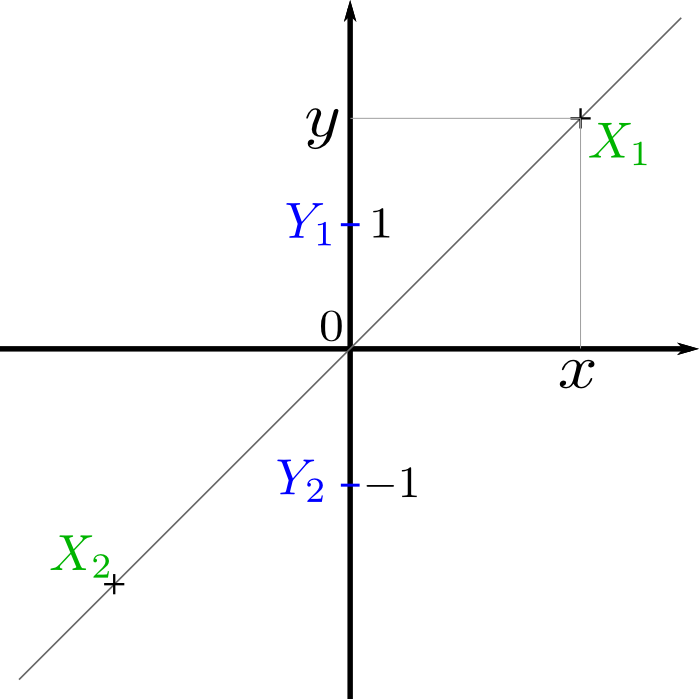
\includegraphics[width=\linewidth]{2diracs/Illustration_deux_points_symetrique_2D}
\end{minipage}
\hfill
\begin{minipage}[p]{0.79\linewidth}
\begin{tabular}{c@{}c@{}c@{}} % @{}c@{}
%\multirow{2}{*}{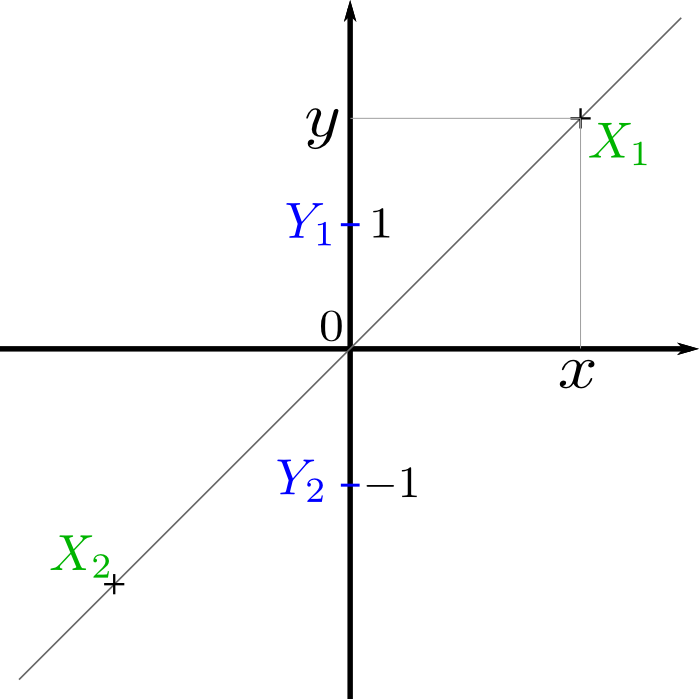
\includegraphics[width=0.24\linewidth]{2diracs/Illustration_deux_points_symetrique_2D}\vspace*{0.12\linewidth}} &
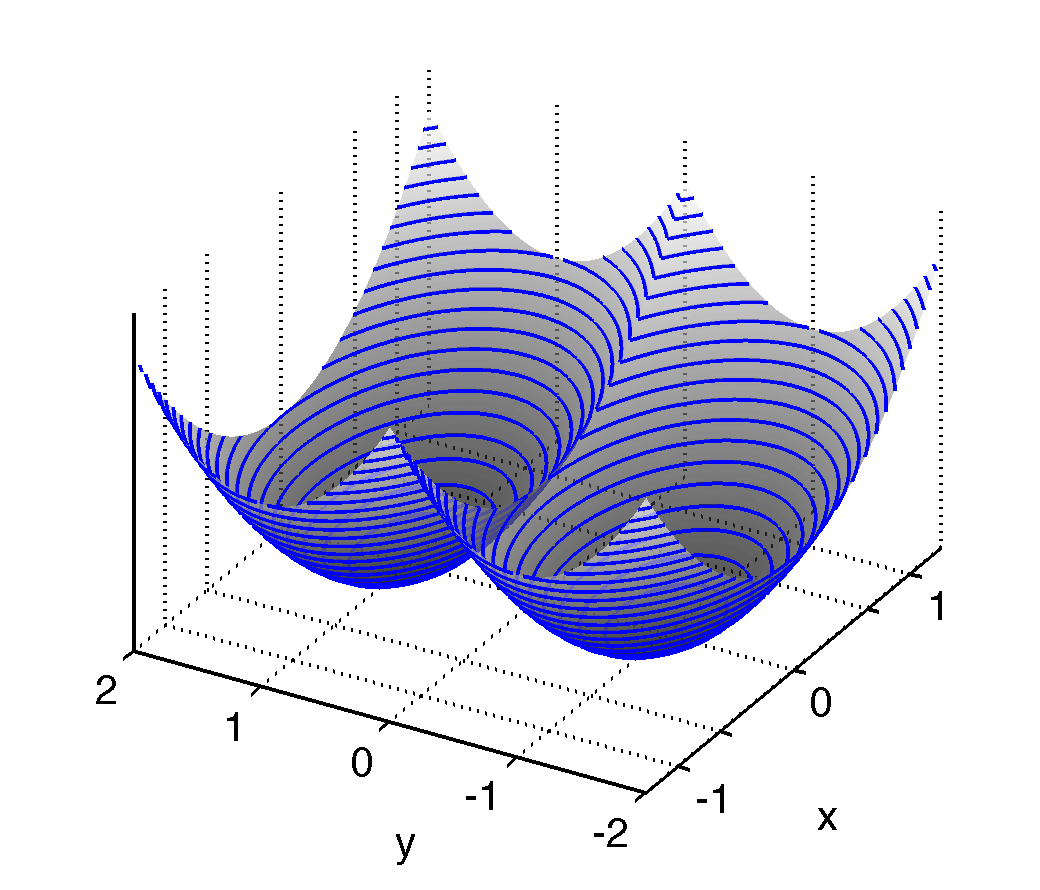
\includegraphics[width=0.33\linewidth]{2diracs/surf_W2_v3}&
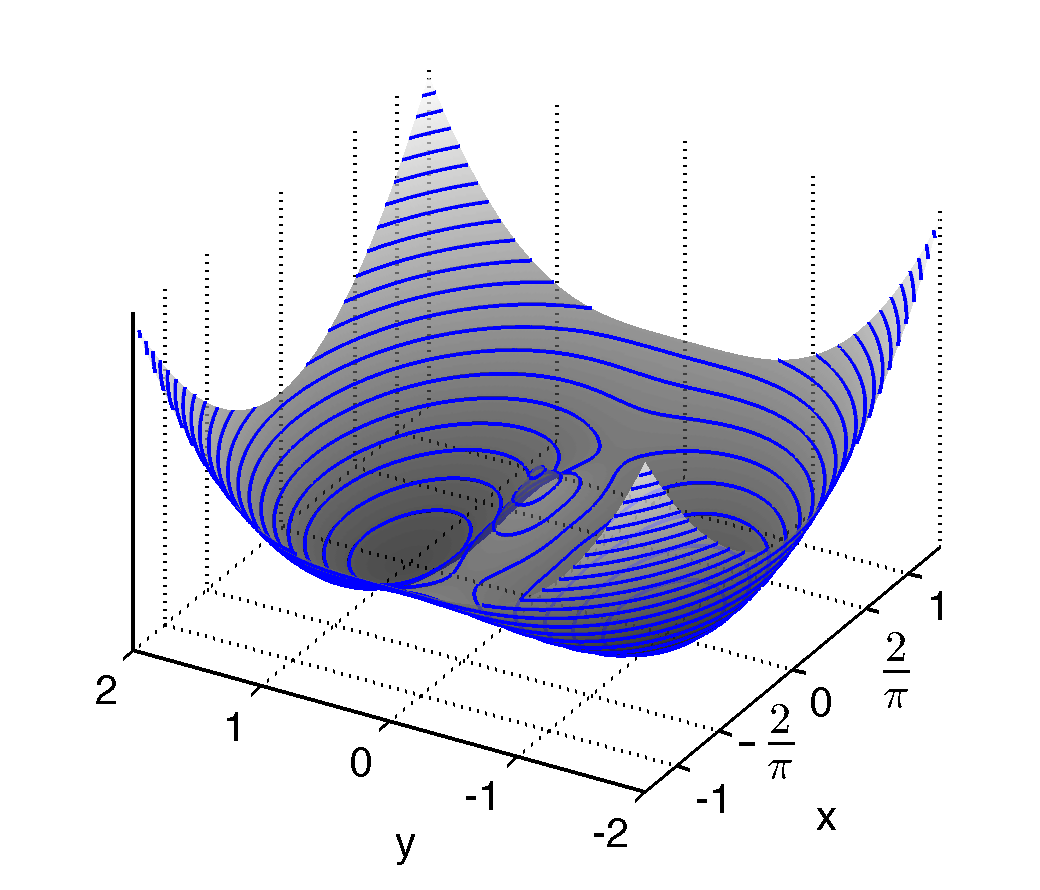
\includegraphics[width=0.33\linewidth]{2diracs/surf_SW2_v3}&
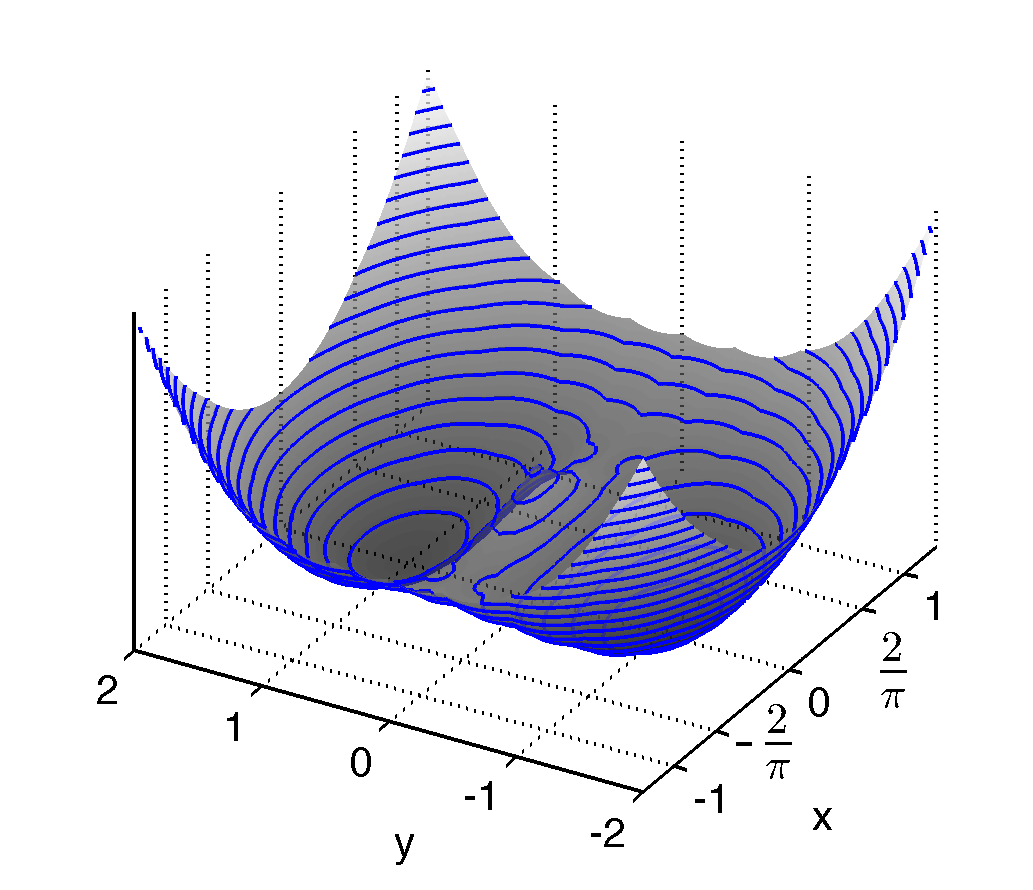
\includegraphics[width=0.33\linewidth]{2diracs/surf_SW2_10dir_v3}
\\
%&
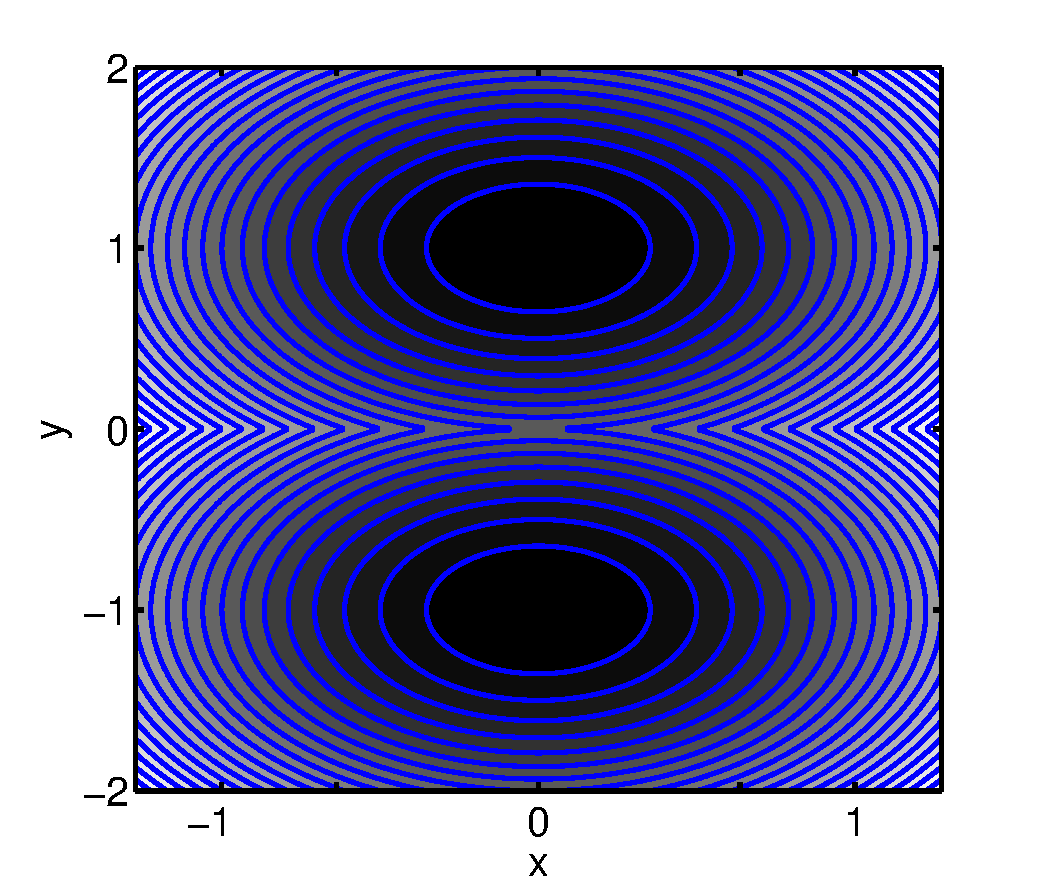
\includegraphics[width=0.33\linewidth]{2diracs/contour_W2_v3}&
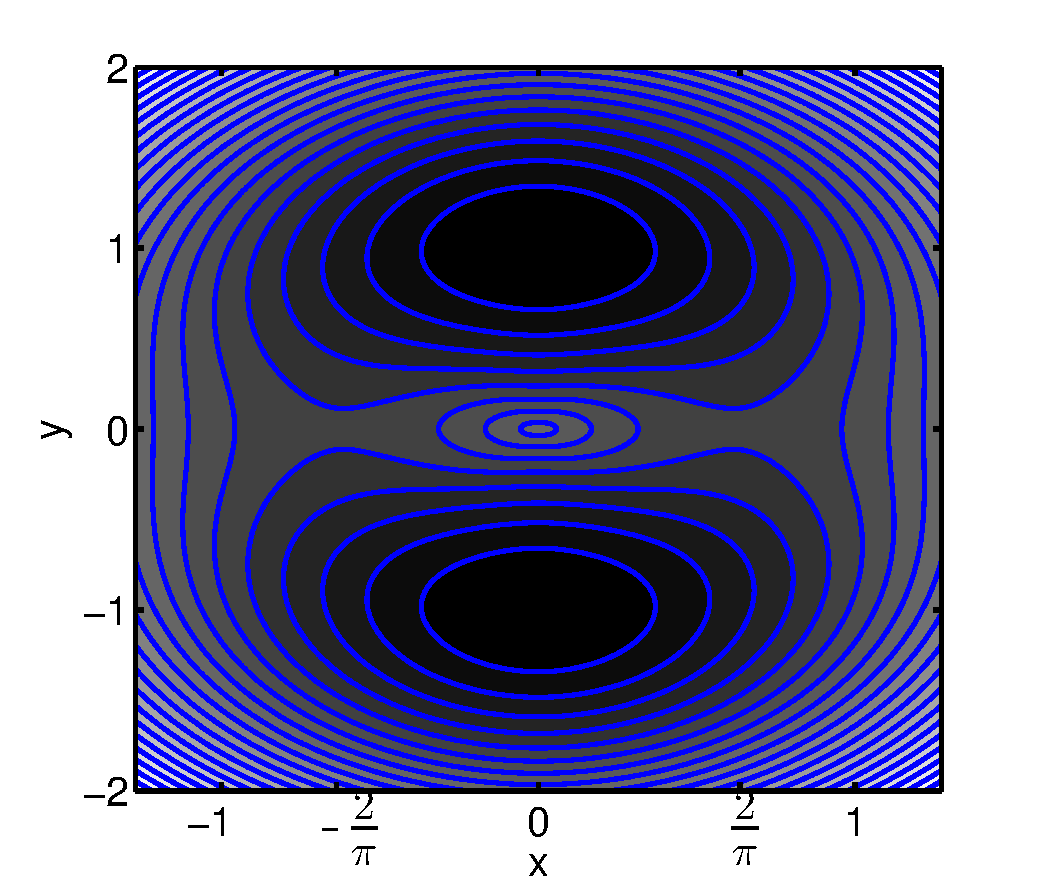
\includegraphics[width=0.33\linewidth]{2diracs/contour_SW2_v3}&
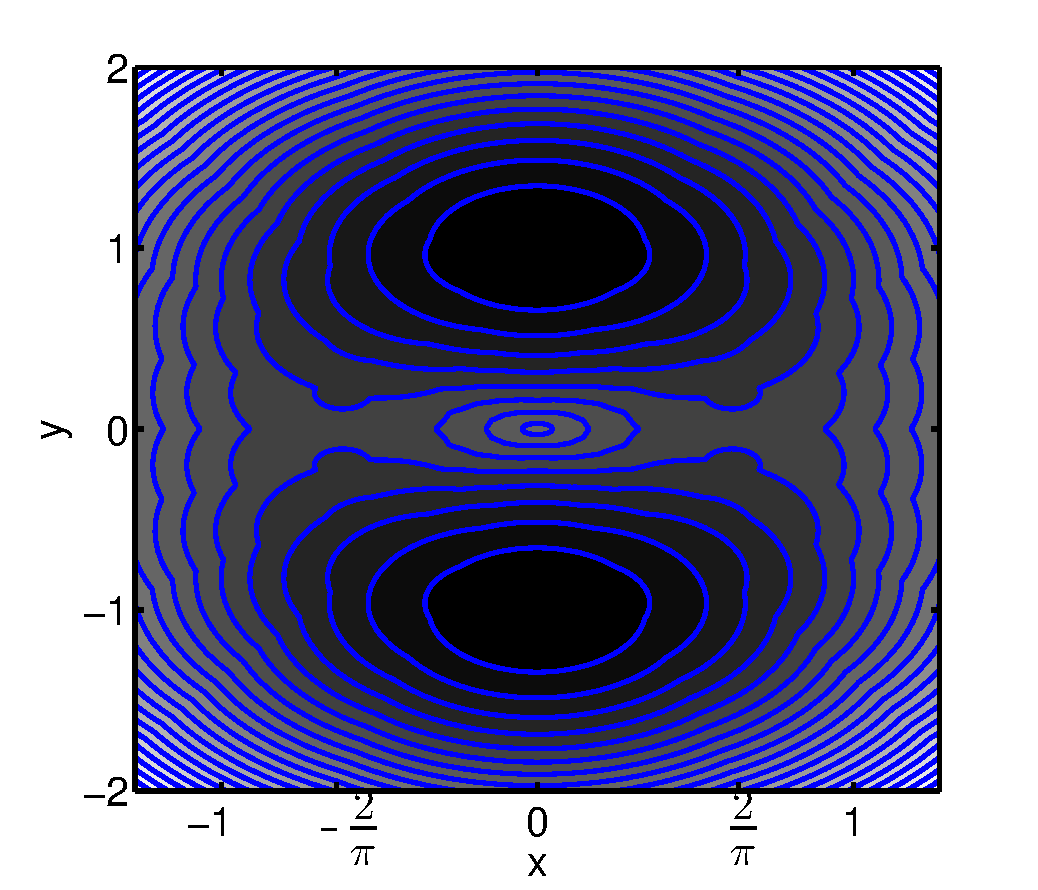
\includegraphics[width=0.33\linewidth]{2diracs/contour_SW2_10dir_v3}
\\
%&
$\Ee^{W}(x,y)$ & $\Ee^{S}(x,y)$ & $\Ee^{S}_\Theta(x,y)$ with $|\Theta|=10$.
\end{tabular}
\end{minipage}
\end{center}
\caption{Comparison of $\SWass{\RR^2}^2$ and $\SWass{\RR^2}^2$, and its numerical approximation using 10 directions, as an elevation surface (top row) and its corresponding 2d map (bottom row).}
\label{fig-comparison}
\end{figure*}



%%%%%%%%%%%%%%%%%%%%%%%%%%%%%%%%%%%%%%%%%%%%%%%%%%%%%%%%%%%%%%%%
\subsection{Numerical Considerations for the Sliced Transport}
\label{subsec-num-stochastic}


%%%%%
\newcommand{\mydisplay}[1]
{
%
\hline &\\
Ref. &
\begin{tabular}{c@{\hspace{6mm}}c@{\hspace{6mm}}c@{}}
\includegraphics[width=0.18\linewidth]{interp_stochastic/#1_mu_1}&
\includegraphics[width=0.18\linewidth]{interp_stochastic/#1_mu_W2bary}&
\includegraphics[width=0.18\linewidth]{interp_stochastic/#1_mu_2}
\\
 $\mu_0$ & $\mu^{W}_\frac{1}{2}$   & $\mu_1$
\end{tabular}
\\
$\mu^{S}_\frac{1}{2}$ &
\begin{tabular}{c@{\hspace{2mm}}c@{\hspace{2mm}}c@{\hspace{2mm}}c@{}}
\includegraphics[width=0.18\linewidth]{interp_stochastic/#1_mu_SW2interp_2dir}&
\includegraphics[width=0.18\linewidth]{interp_stochastic/#1_mu_SW2interp_20dir}&
\includegraphics[width=0.18\linewidth]{interp_stochastic/#1_mu_SW2interp_200dir}&
\includegraphics[width=0.18\linewidth]{interp_stochastic/#1_mu_SW2interp_2000dir}
\\
$\abs{\Th_\ell}=2$ &
$\abs{\Th_\ell}=20$ &
$\abs{\Th_\ell}=200$ &
$\abs{\Th_\ell}=2000$
\end{tabular} \\
%
}
%%%%%

\begin{figure}[!t]
\begin{center}
\begin{tabular}{|c|c|}
%
\mydisplay{48701}
\mydisplay{117925}
\mydisplay{799530}
%
\\
\hline
\end{tabular}
\end{center}
\caption{ %\textit{Influence of the $\Sph$ discretization for the Sliced Wasserstein transport.}
We consider the optimal Wasserstein barycenter $\mu^{W}_\frac{1}{2}$ between $\mu_0$ and $\mu_1$.
We show the Sliced Wasserstein interpolation $\mu^{S}_\frac{1}{2}$ using our stochastic Newton descent \eqref{eq-stoch-grad-desc} %\eqref{eq-grad-desc-sliced_newton}.
with different number of directions $\abs{\Th_\ell}$. The density is displayed using a Parzen density estimation.
}
\label{fig:interp_stochastic}
\end{figure}

\paragraph{Influence of the number of directions. } 

We first illustrate the special case discussed in Section~\ref{subsec-sliced-assignement} of the transport of a discrete distribution (a sum of Dirac masses) $\mu_0$ toward another, $\mu_1$. This boils down to an assignment problem. We resort to the stochastic gradient descent detailed in \eqref{eq-stoch-grad-desc} to compute a Sliced Wasserstein transport $T^S$.
This map $T^S$ always numerically verifies $T^S\#\mu_0 = \mu_1$. Nevertheless, it can be far from the optimal Wasserstein transport map $T^W$ when using a small number of directions at each iteration.
We illustrate this in Figure~\ref{fig:interp_stochastic}, that shows the distributions obtained when interpolating the transport map $T^S$, that is, we compute $\mu_{\lambda}^S = [(1-{\lambda}) \Id +  \lambda T^S] \sharp \mu_0$ for $\la \in [0,1]$, when varying the number of directions $\Th_\ell$ used at each iteration.
Using more sampling directions tends to provide more regular transport maps.  However, we note that the Sliced Wasserstein transport can provide a different assignment from the optimal Wasserstein map, even when using a large set of directions (Fig.~\ref{fig:interp_stochastic}, third example).

%%%
\paragraph{Influence of local minima.} 

Since the algorithm detailed in Section~\ref{subsec-algorithm-lagrangian} performs a non-convex energy minimization (see~\eqref{eq-non-convx-pointclouds}), it is important to understand the influence of the initialization of the descent. Figure~\ref{fig:rnd_init} analyzes on a simple example the effect of the presence of local minima. The center plots (b) and (c) each show two results (blue and red dots) approximating the sliced iso-barycenter $\mu^S_{1/2}$ %(middle point of the geodesic) \cmt{at this stage, we have already used it a lot, and the definition is obvious}
%\eq{
	%\mu_{1/2} = \Bary{\RR^d}^S \left( (\mu_0,\mu_1), (\tfrac{1}{2},\tfrac{1}{2}) \right).
%}
using our non-convex gradient descent, as well as the Wasserstein barycenter $\mu^W_{1/2}$ (black dots) computed via linear programming since there are only two distributions. 
Each result is obtained using a random initialization with samples independently drawn from an isotropic Gaussian having the same mean and variance as $\mu_0$. While this clearly shows that different initializations lead to different estimates, this also shows that the impact of the initialization is quite modest. 


\begin{figure*}[!t]
\begin{center} 
\begin{tabular}{@{}c@{\hspace{5mm}}c@{\hspace{5mm}}c@{\hspace{5mm}}c@{}}
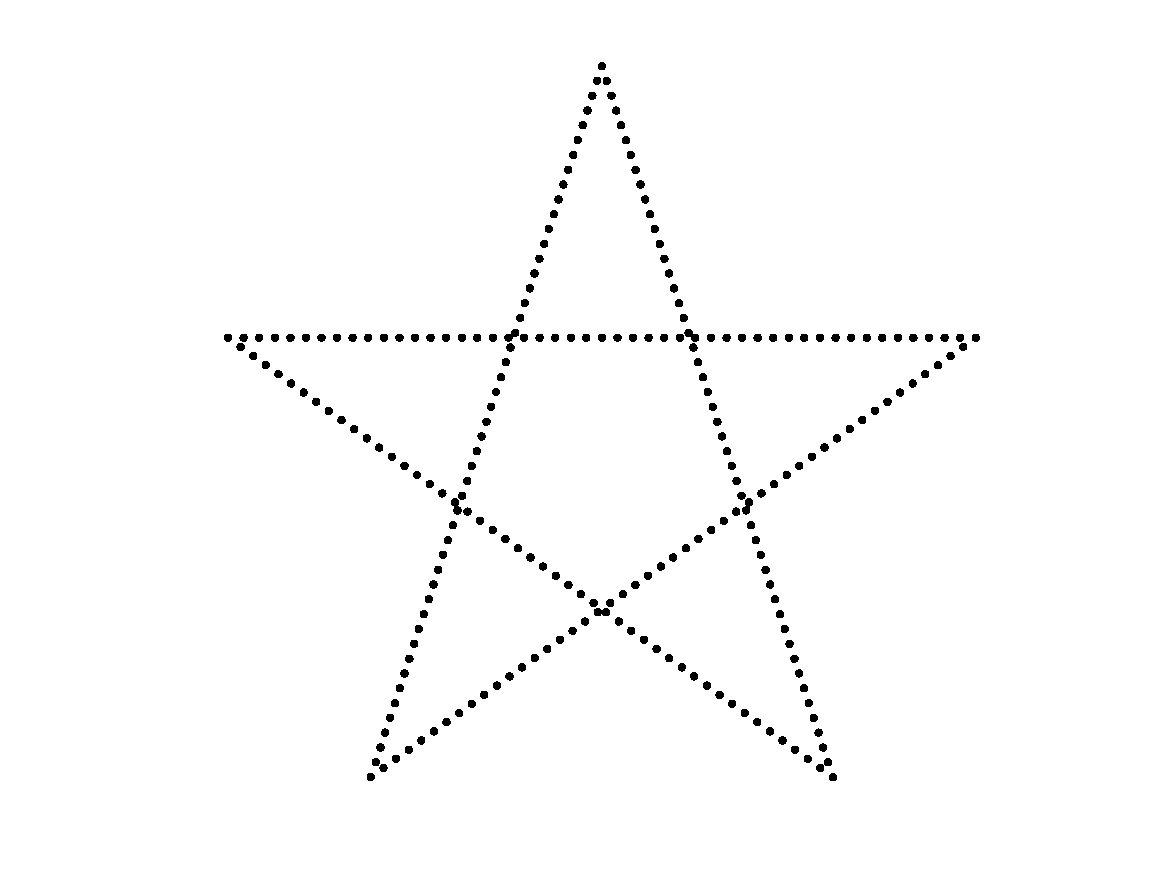
\includegraphics[width=0.23\linewidth]{init/star_v1}&
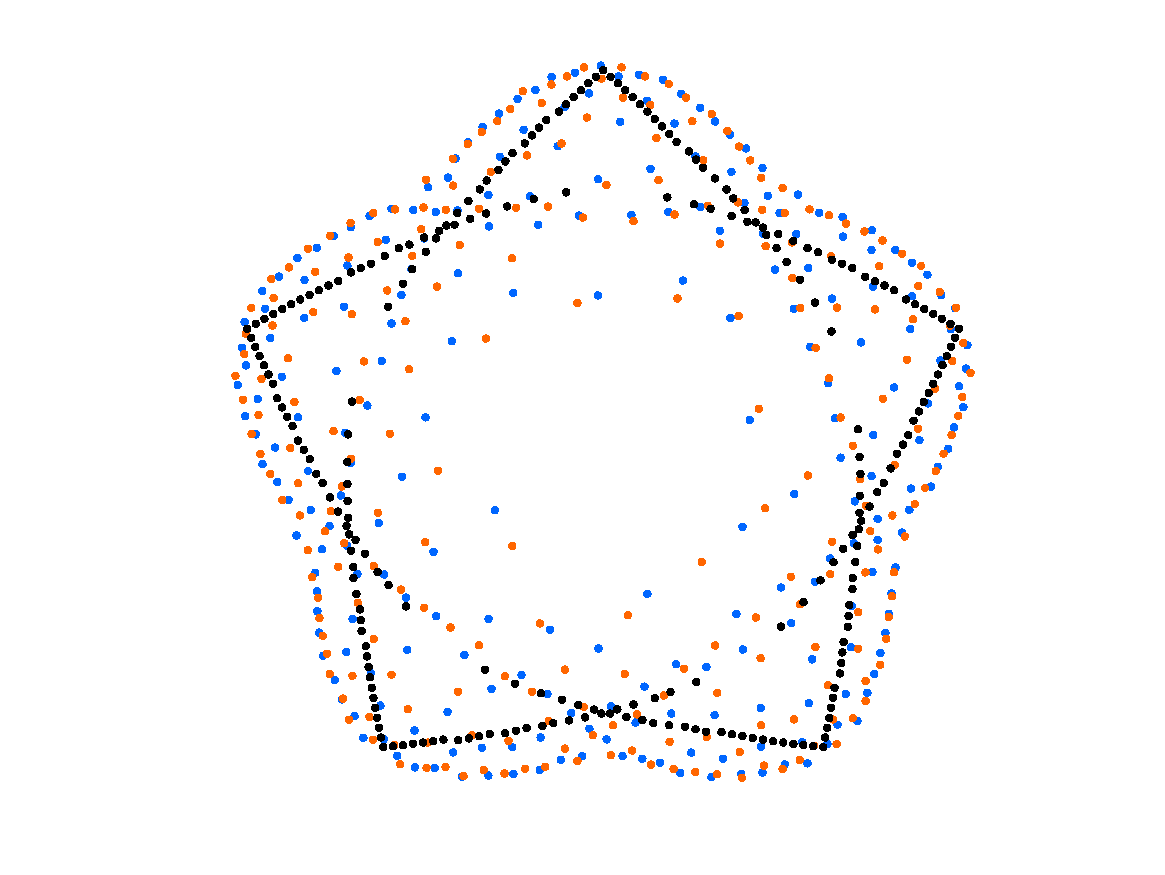
\includegraphics[width=0.22\linewidth]{init/circle_star_sw_bary_rnd_init_1000_v1}&
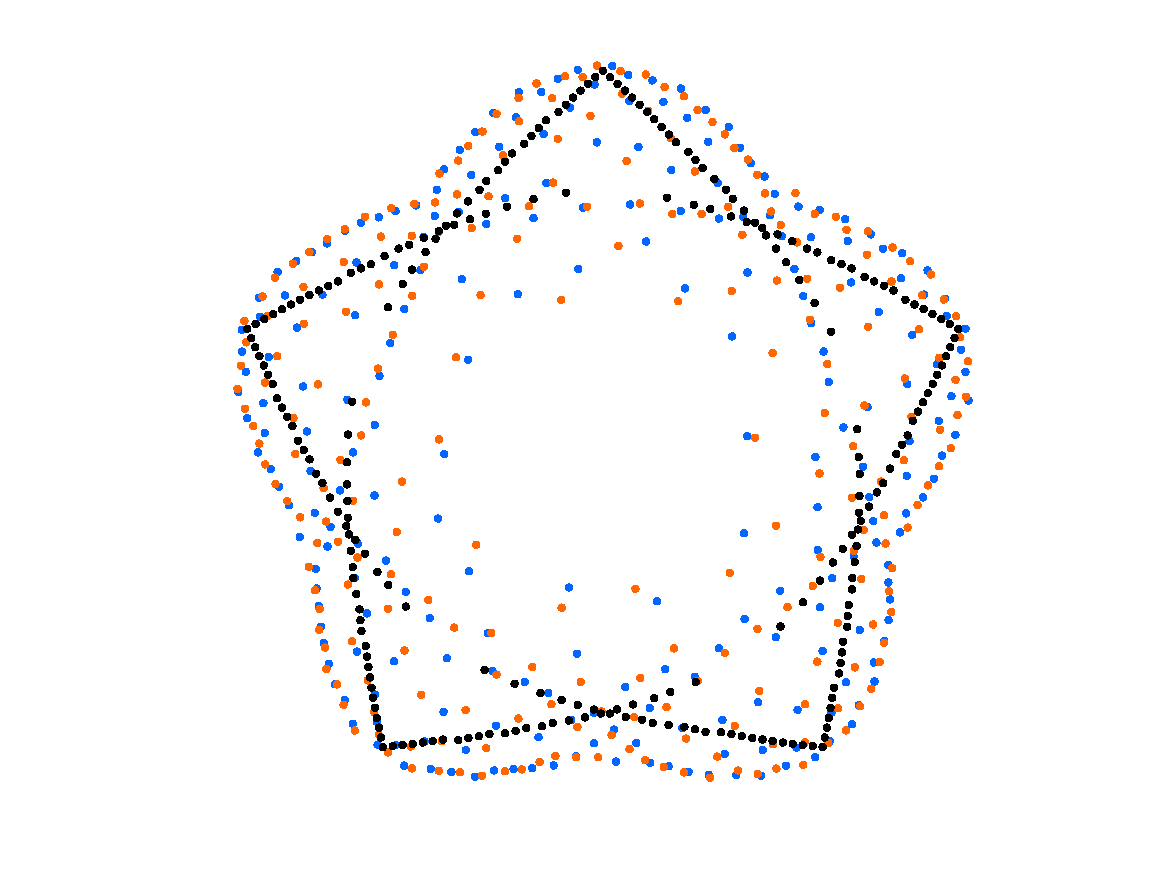
\includegraphics[width=0.22\linewidth]{init/circle_star_sw_bary_rnd_dir_1000_v1}&
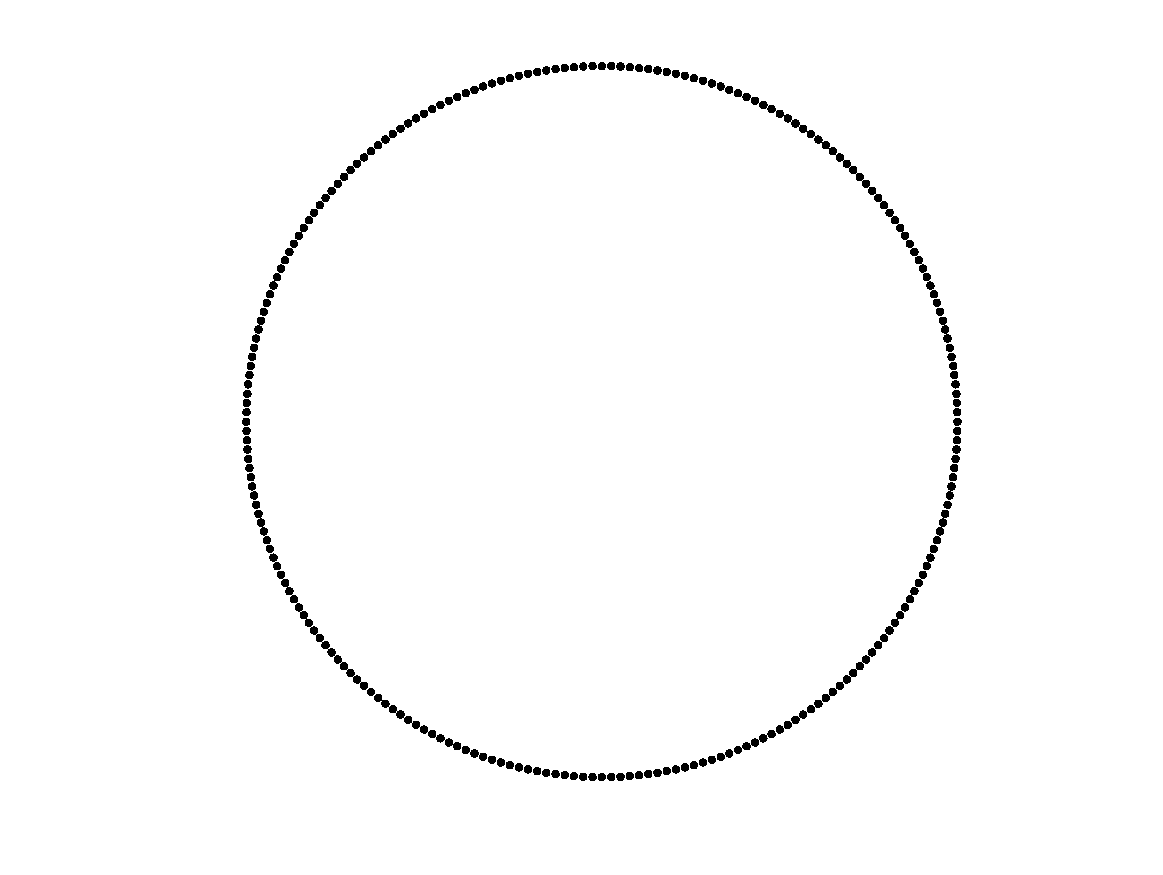
\includegraphics[width=0.22\linewidth]{init/circle_v1}\\
(a) $\mu_0$  & (b) $\mu^S_{1/2}$ (uniform $\Th$) & (c) $\mu^S_{1/2}$ (random $\Th$) & (d) $\mu_1$
\end{tabular}
\end{center}
\caption{ Influence of the initialization $X^{[0]}$ and the directions set $\Theta$ (here $\lvert\Theta\rvert=10^3$) on our Lagrangian discretization of the sliced barycenter. 
The black point cloud corresponds to the Wasserstein interpolation $\mu^W_{1/2}$ of the two distributions $\mu_0$ and $\mu_1$.  The red and blue point clouds correspond to the sliced Wasserstein barycenters obtained with different settings: (b) using two random point 
clouds initializations for $X^{[0]}$ with the same set of directions $\Theta$ (equi-spaced on the circle);  (c) using the same initializations $\mu_{X^{[0]}} = \mu_0$ but with different uniformly sampled random directions $\Theta$.}
\label{fig:rnd_init}
\end{figure*}



%%%%%%%%%%%%%%%%%%%%%%%%%%%%%%%%%%%%%%%%%%%%%%%%%%%%%%%%%%%%%%%%
\subsection{Numerical Comparison of the Barycenters}
\label{subsec-num-comparison}

This section compares the following barycenters in a 2-D ($d=2$) setting:
\begin{itemize}
	\item[--] The original Wasserstein barycenter $\Bary{\RR^d}^W$ (see Definition~\ref{defn-wass-baryc}), which can only be computed numerically for $2$ distributions, i.e. $|I|=2$, and thus corresponds to the Wasserstein geodesic between the two measures. We use the proximal splitting method of~\cite{FPapPeyOud13} to estimate this barycenter with a Eulerian discretization on a fixed grid.	%\todo{and which approach for the Lagrangian version? (in Fig.2) : I used Hungarian Algorithm for small point clouds and Mosek library for larger point clouds (simplex or interior point primal-dual methods)} 
	\item[--] The Radon barycenter $\Bary{\RR^d}^R$ (see Definition~\ref{defn-radon-baryc}). It is approximated with the numerical scheme presented in Section~\ref{subsec-algorithm-eulerian} with an Eulerian discretization. 
	\item[--] The sliced barycenter $\Bary{\RR^d}^S$ (see Definition~\ref{defn-sliced-baryc}). It is approximated with the numerical scheme presented in Section~\ref{subsec-algorithm-lagrangian} with a Lagrangian discretization. If not stated otherwise, we use $|\Theta|=10$ directions uniformly sampled on the half circle. 
\end{itemize}



%%%
\paragraph{Comparison of the Sliced, Radon and Wasserstein Geodesics.} 

In general, the sliced and Radon barycenters differ from the original Wasserstein barycenter. While the Wasserstein barycenter of Gaussian distributions is always a Gaussian distribution~\cite{Carlier_wasserstein_barycenter}, Figure~\ref{fig:aniso} shows that this is not the case for the Radon barycenter when the Gaussians are not isotropic.

\begin{figure}[!t]
\begin{center}
\begin{tabular}{@{}c@{}c@{}c@{}c@{}c@{}}

\includegraphics[width=0.19\linewidth]{gaussian-geod/anis0_padding}&

\includegraphics[width=0.19\linewidth]{gaussian-geod/anis1_padding}&

\includegraphics[width=0.19\linewidth]{gaussian-geod/anis2_padding}&

\includegraphics[width=0.19\linewidth]{gaussian-geod/anis3_padding}&

\includegraphics[width=0.19\linewidth]{gaussian-geod/anis4_padding}\\
$t=0$ & $t=1/4$ & $t=1/2$ & $t=3/4$ & $t=1$
\end{tabular}
\end{center}
\caption{ The Radon geodesic $\mu_t = \Bary{\RR^d}^R( (\mu_0,\mu_1), (t,1-t) )$ between two anisotropic Gaussians is not Gaussian.}
\label{fig:aniso}
\end{figure}

Figure~\ref{fig:compareRef} shows a more detailed comparison of both smooth (Gaussian mixture) and non-smooth (characteristic function of animal-like shapes) densities. Only the edge of the barycentric triangle is available for the Wasserstein barycenter, since there is no efficient algorithm to approximate the Wasserstein barycenter of more than two measures. 

\begin{figure*}[!ht]
\setlength{\tabcolsep}{1pt}
\setlength{\fboxsep}{1pt}
\begin{center} 
\begin{tabular}{c@{\hspace{5mm}}c@{\hspace{5mm}}c@{}}
%\includegraphics[width=0.24\linewidth]{twogauss/twogaussColorsRadon} &
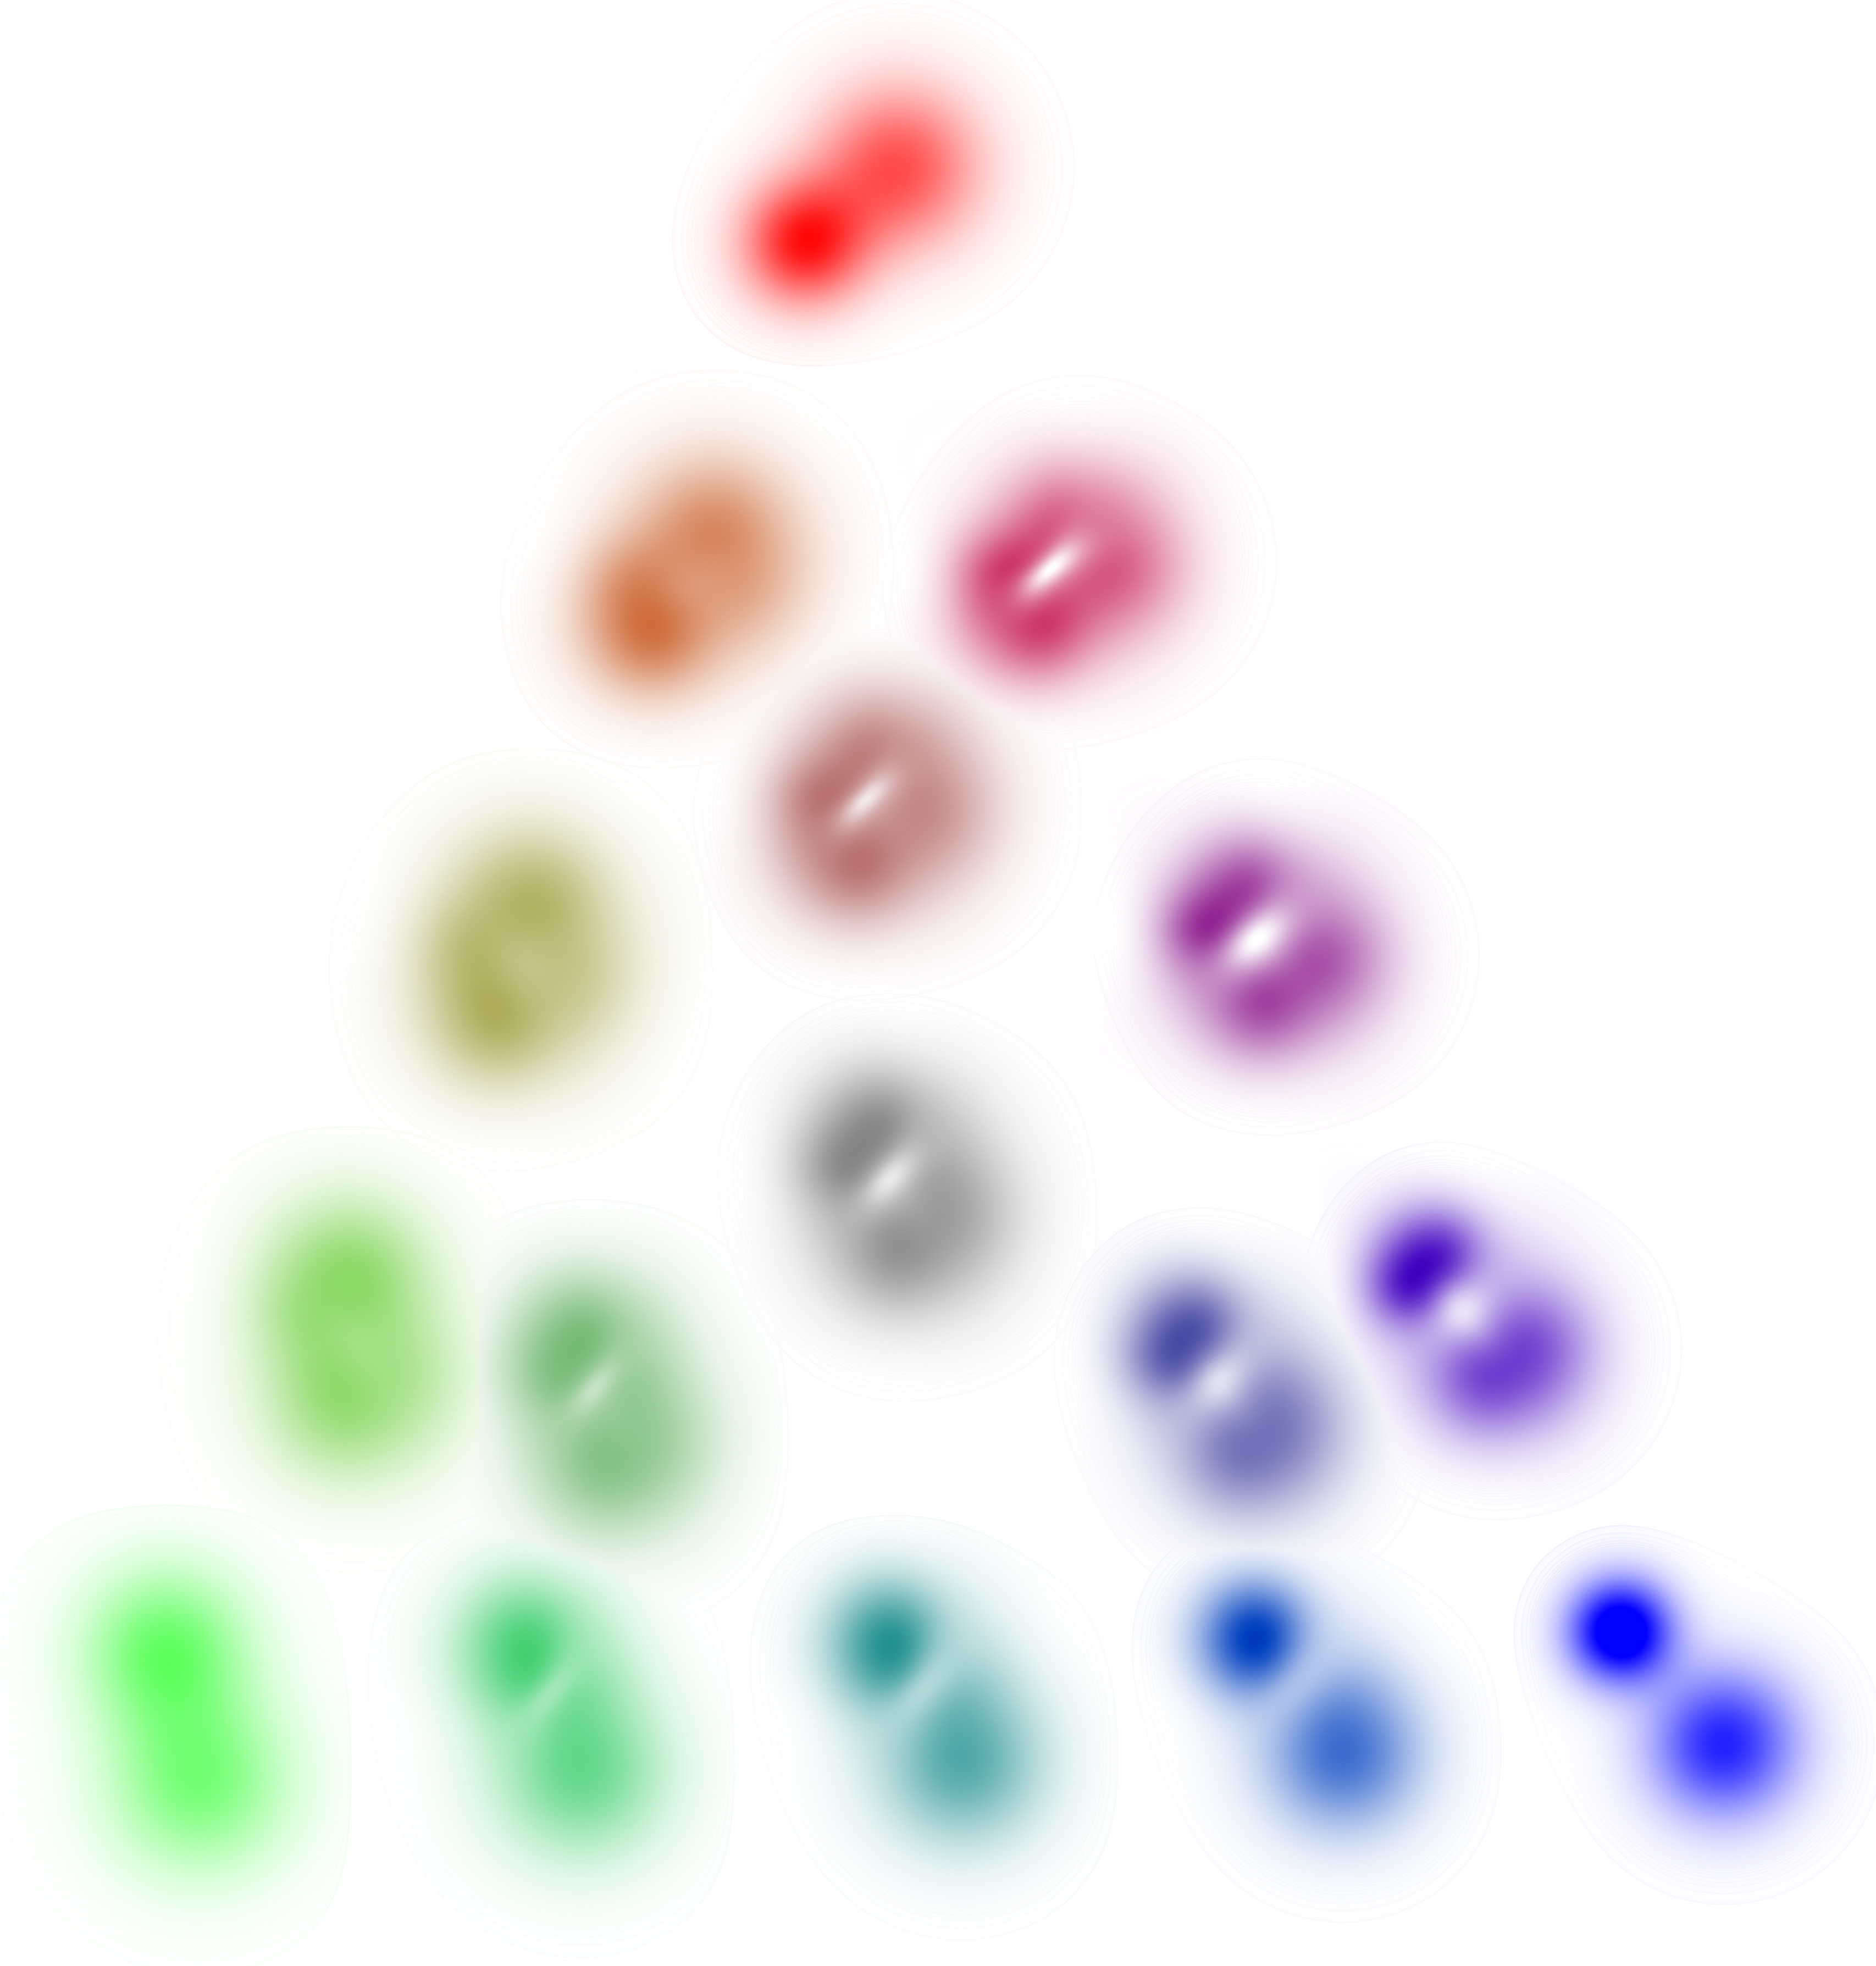
\includegraphics[width=0.31\linewidth]{twogauss/twogaussColorsFastSlant} &
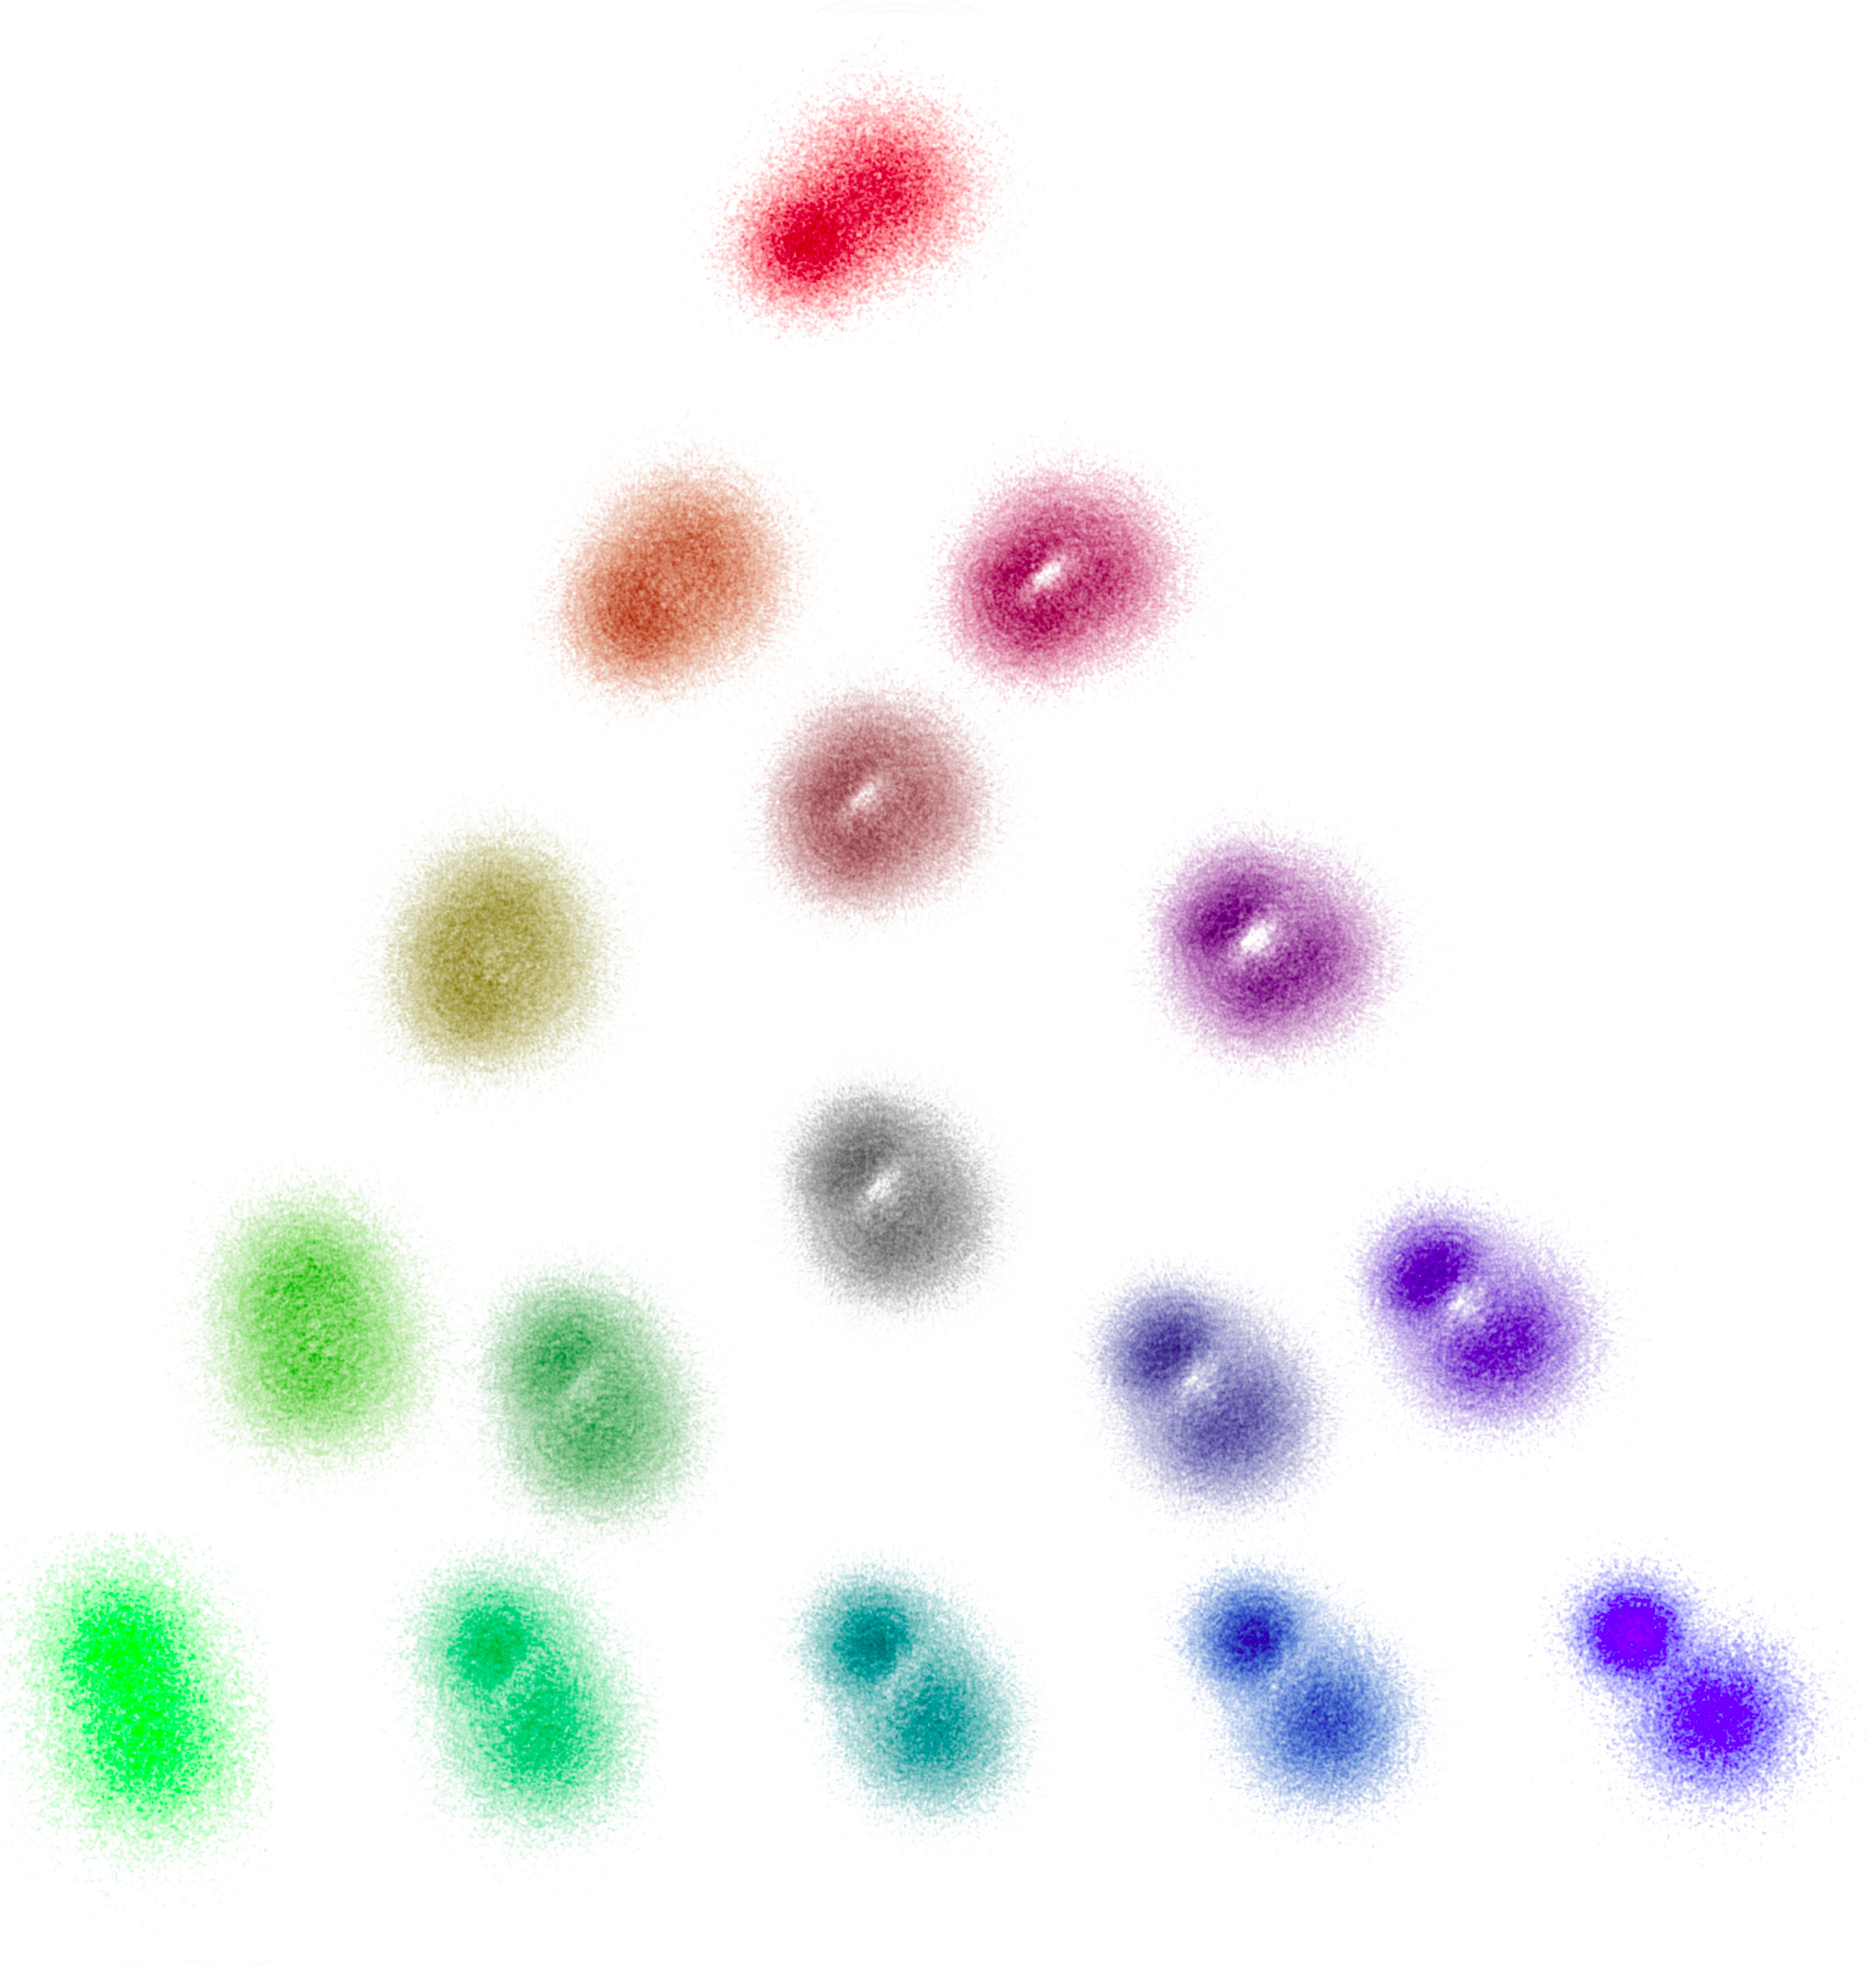
\includegraphics[width=0.31\linewidth]{twogauss/twogaussColorsSliced} &

\includegraphics[width=0.31\linewidth]{twogauss/twogaussColorsRef} \\
%\includegraphics[width=0.24\linewidth]{animals/animalsColorRadon_padded} &
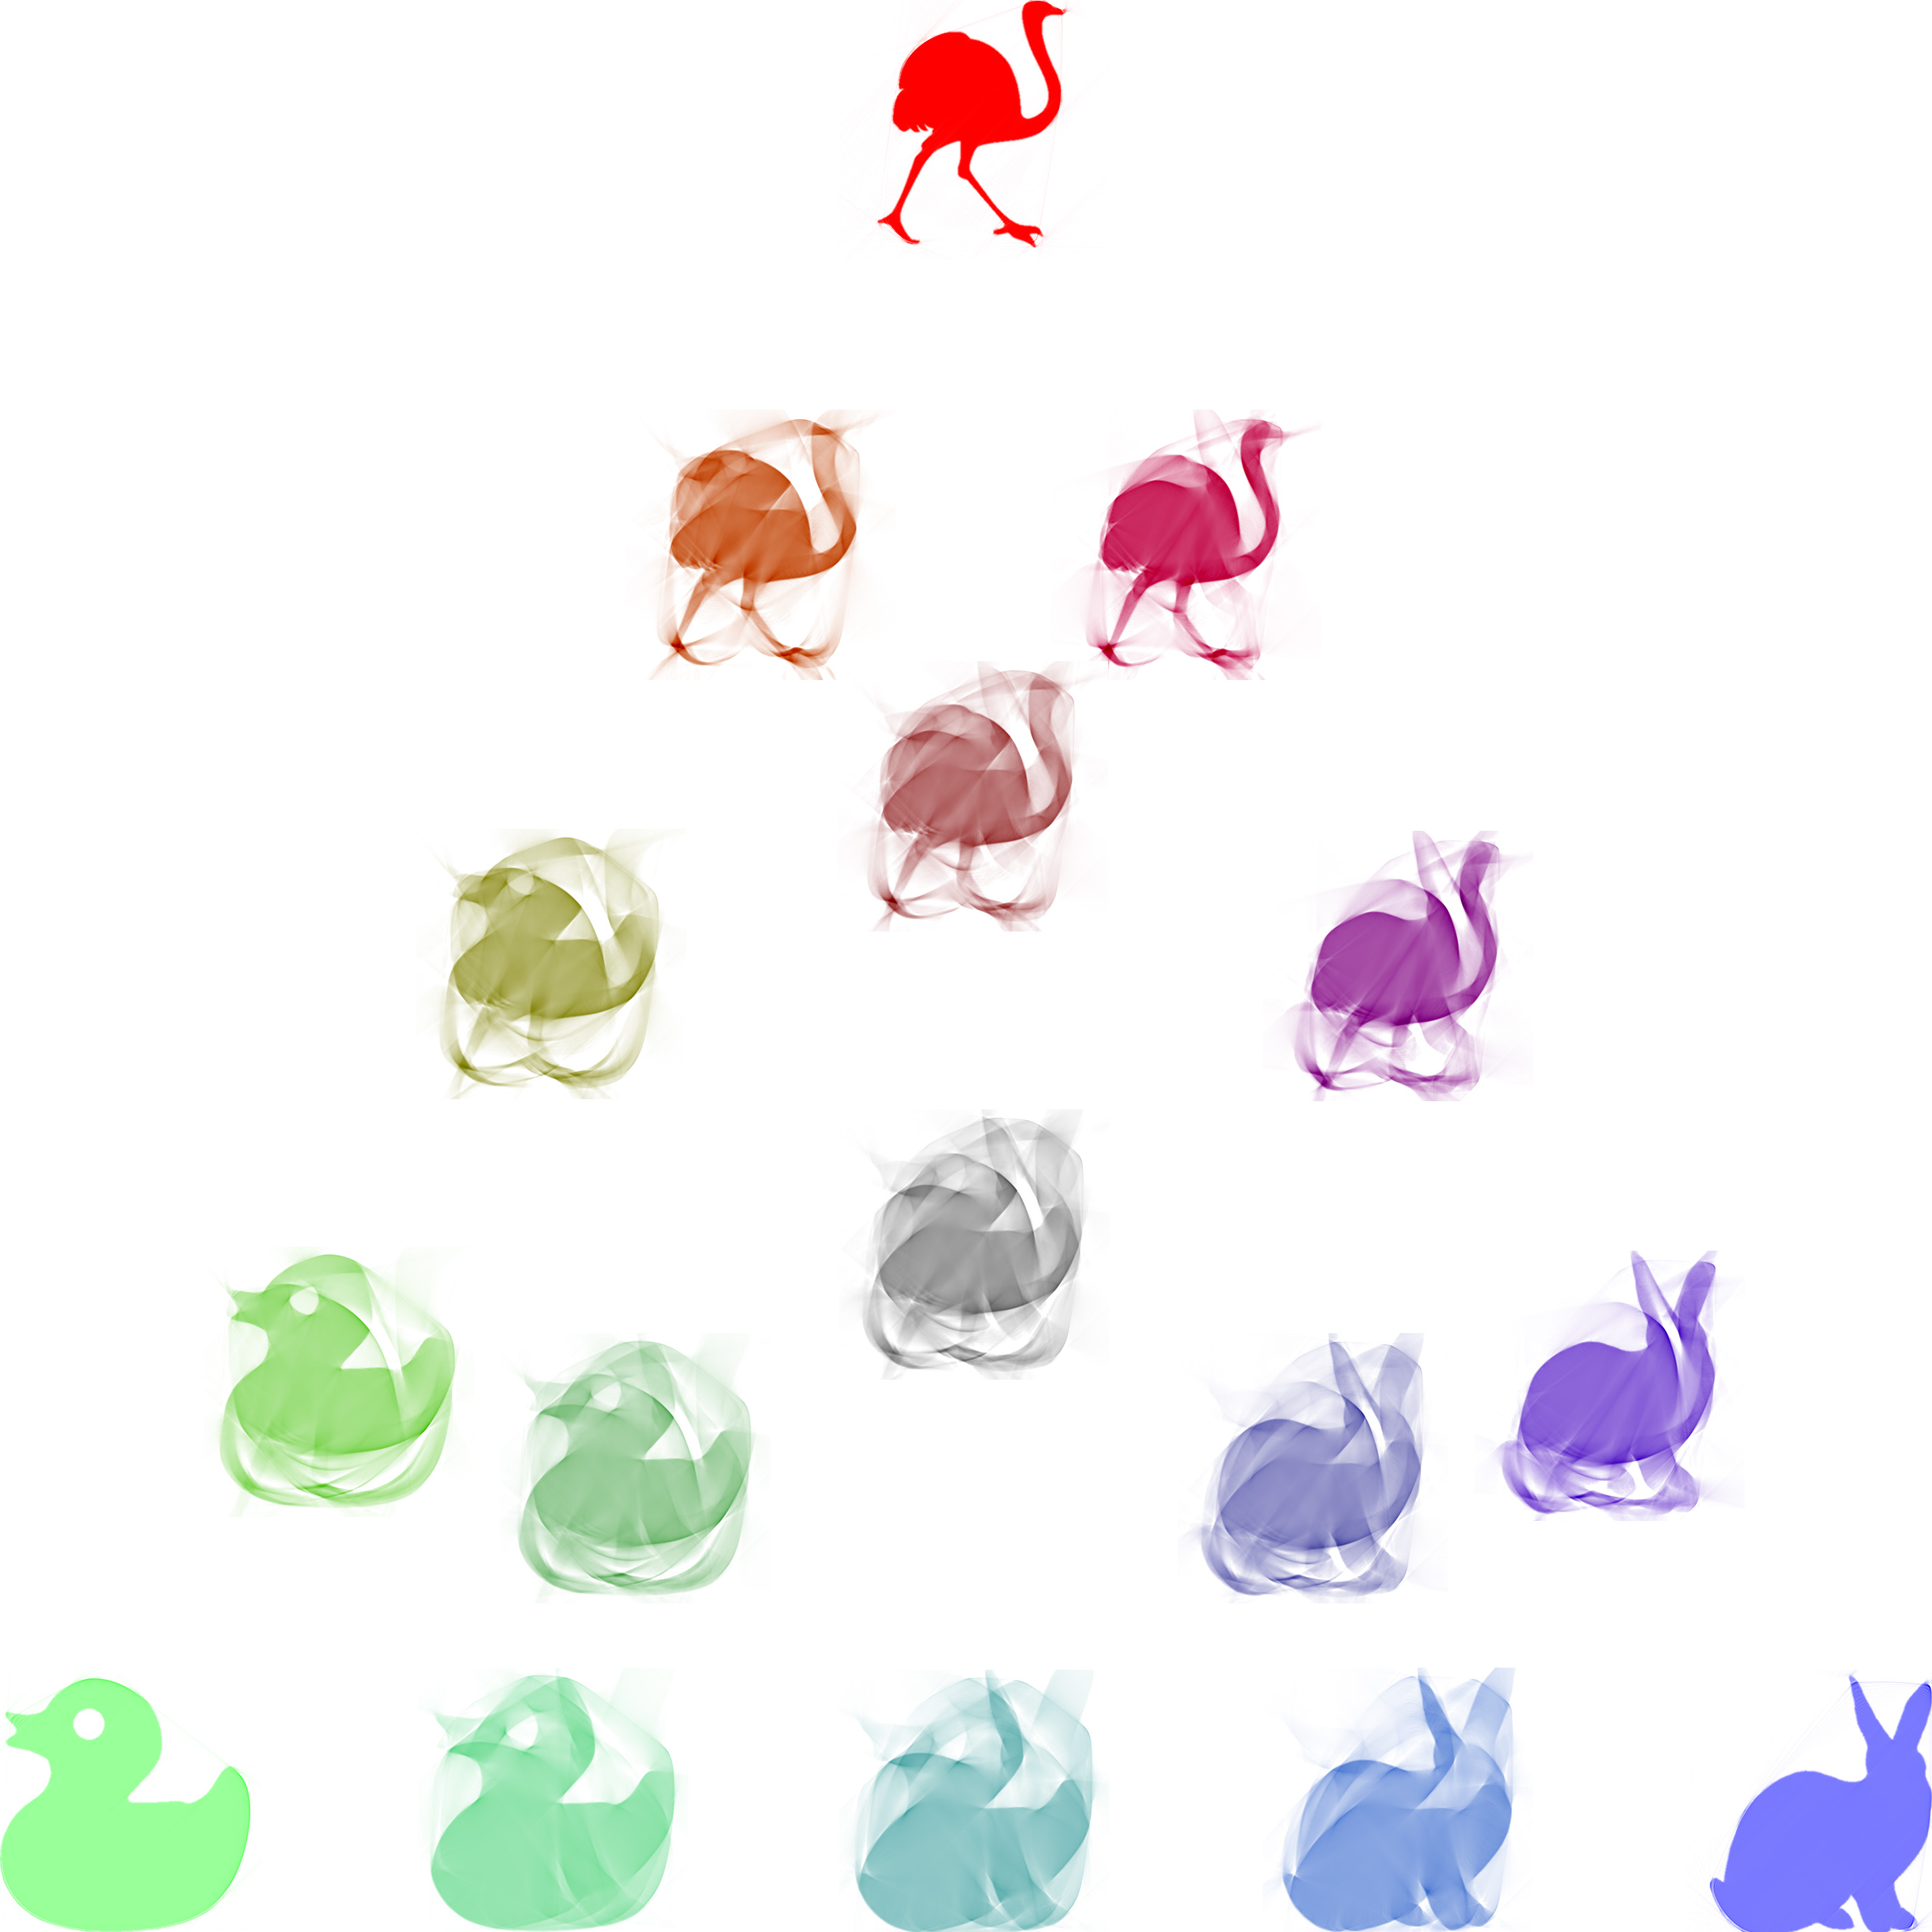
\includegraphics[width=0.31\linewidth]{animals/animalsColorFastSlant_padded} &
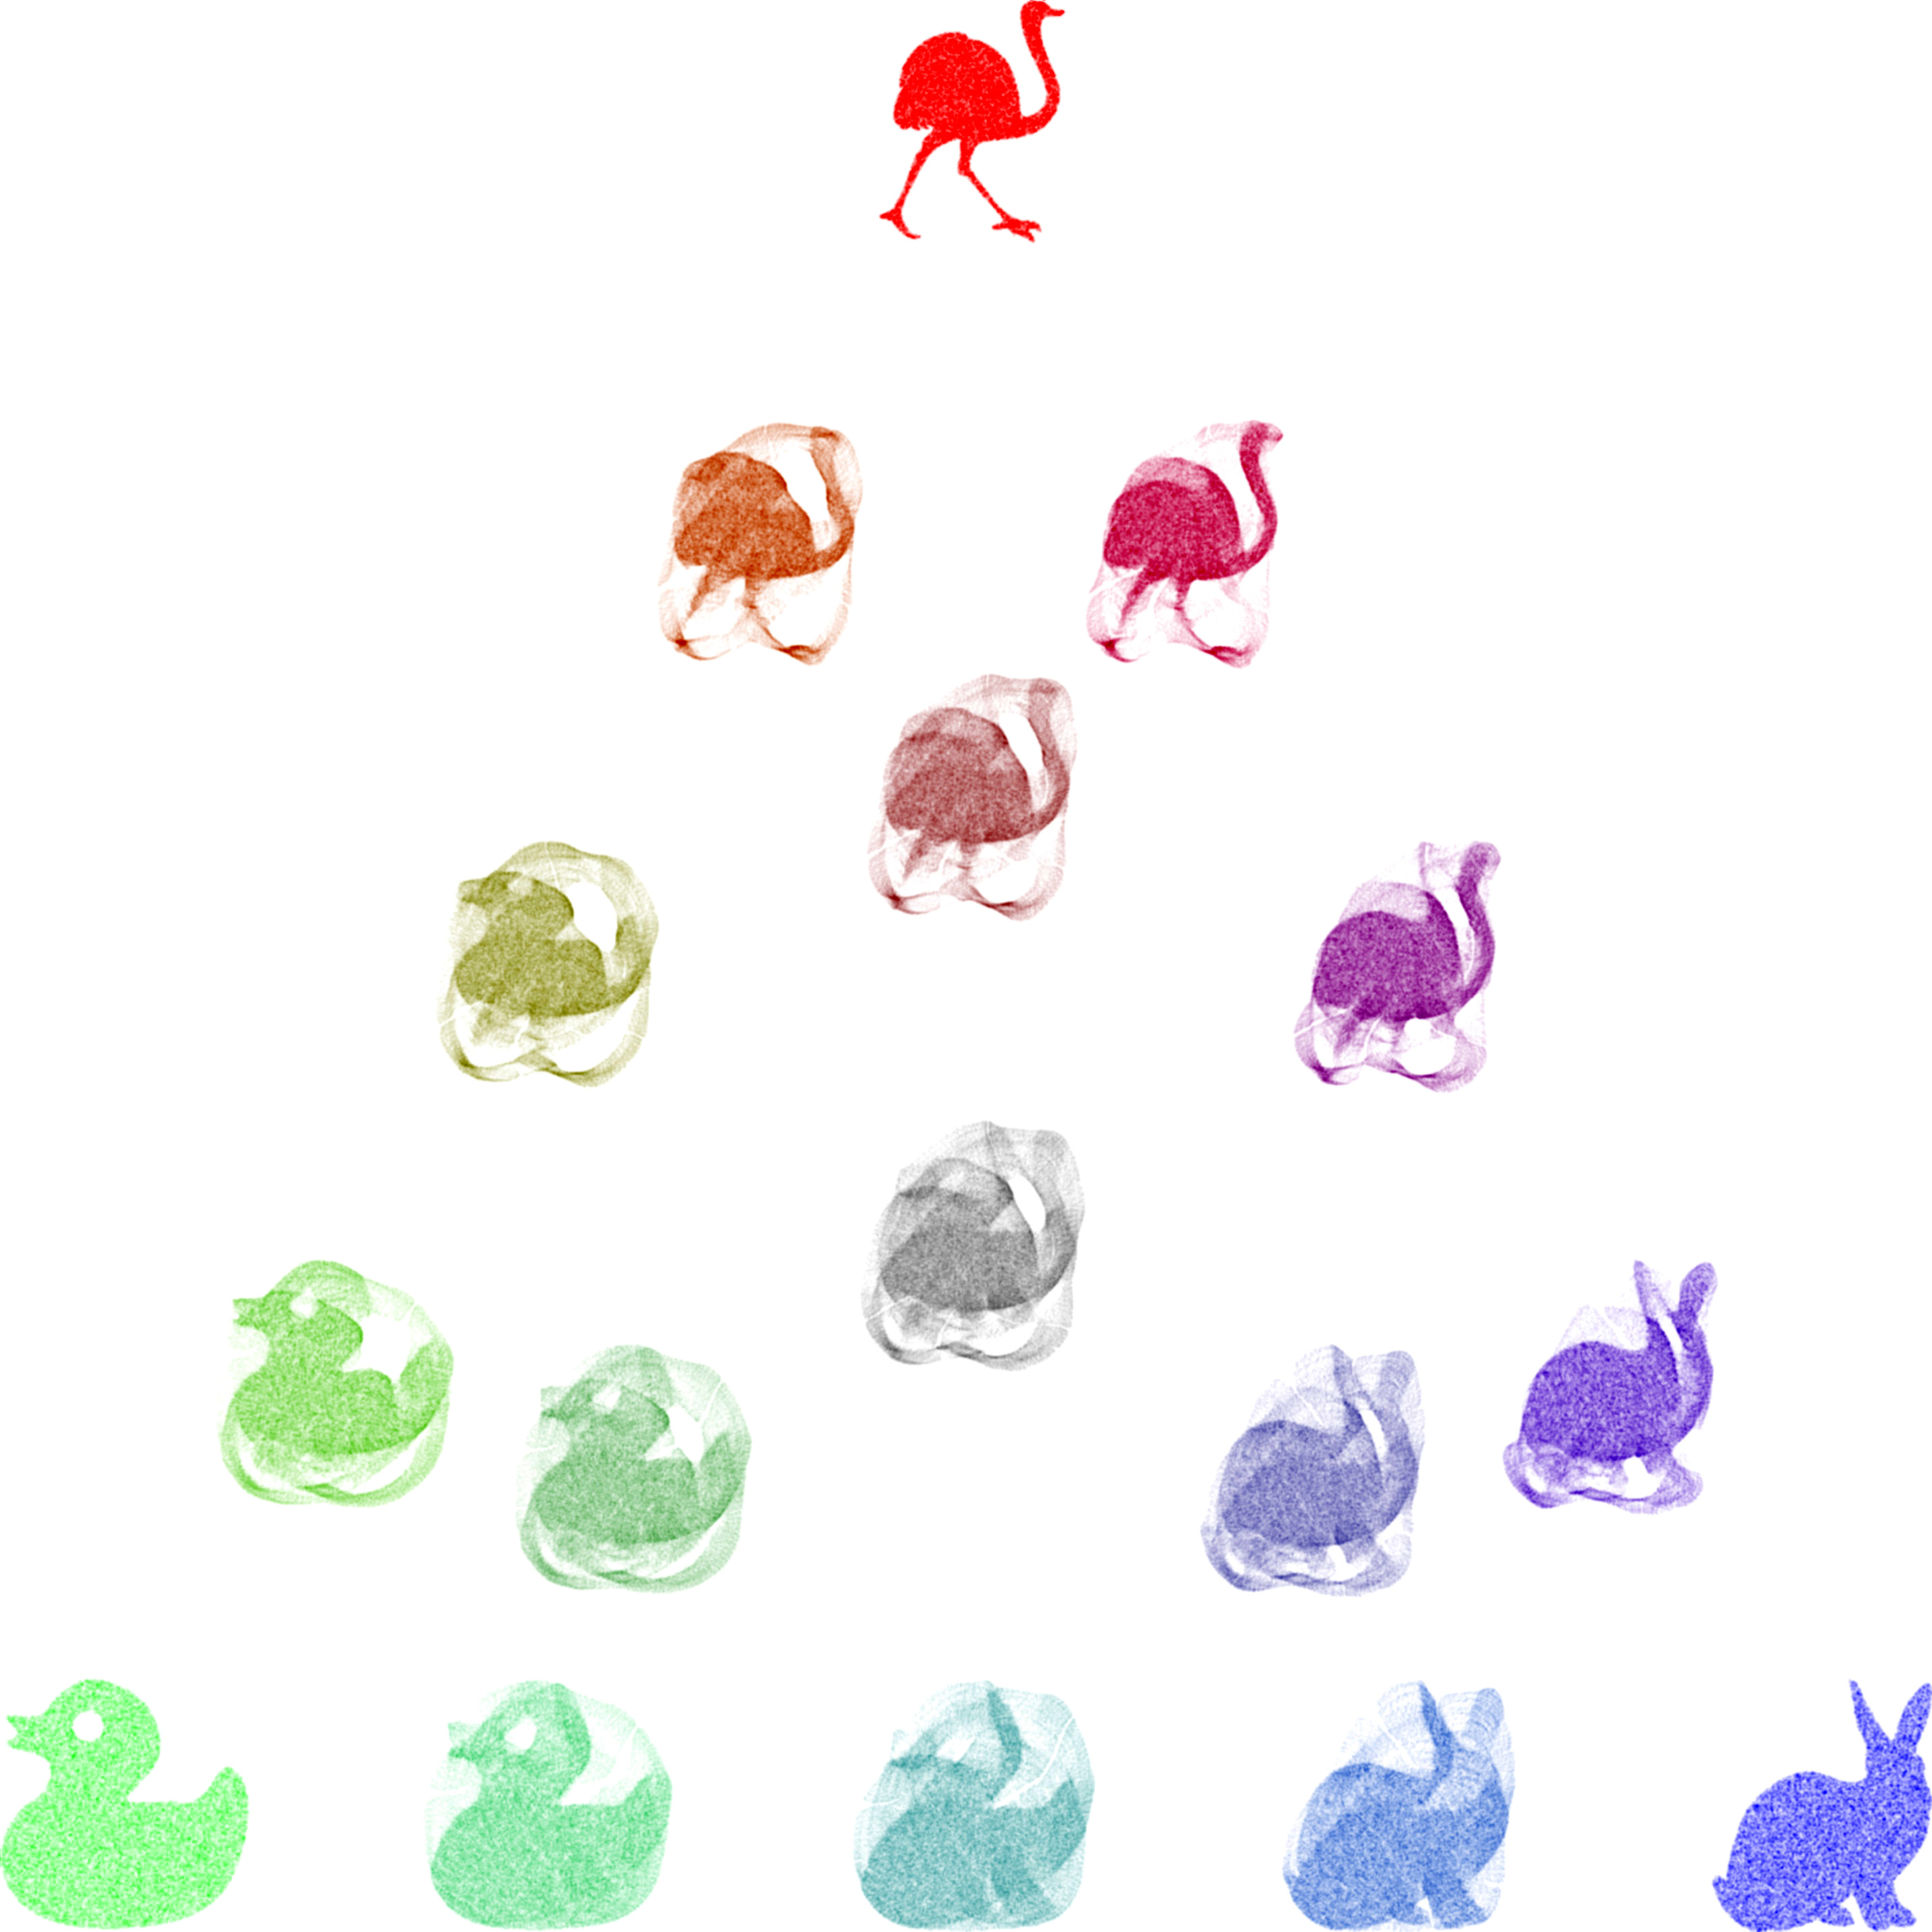
\includegraphics[width=0.31\linewidth]{animals/animalsColorSliced} &
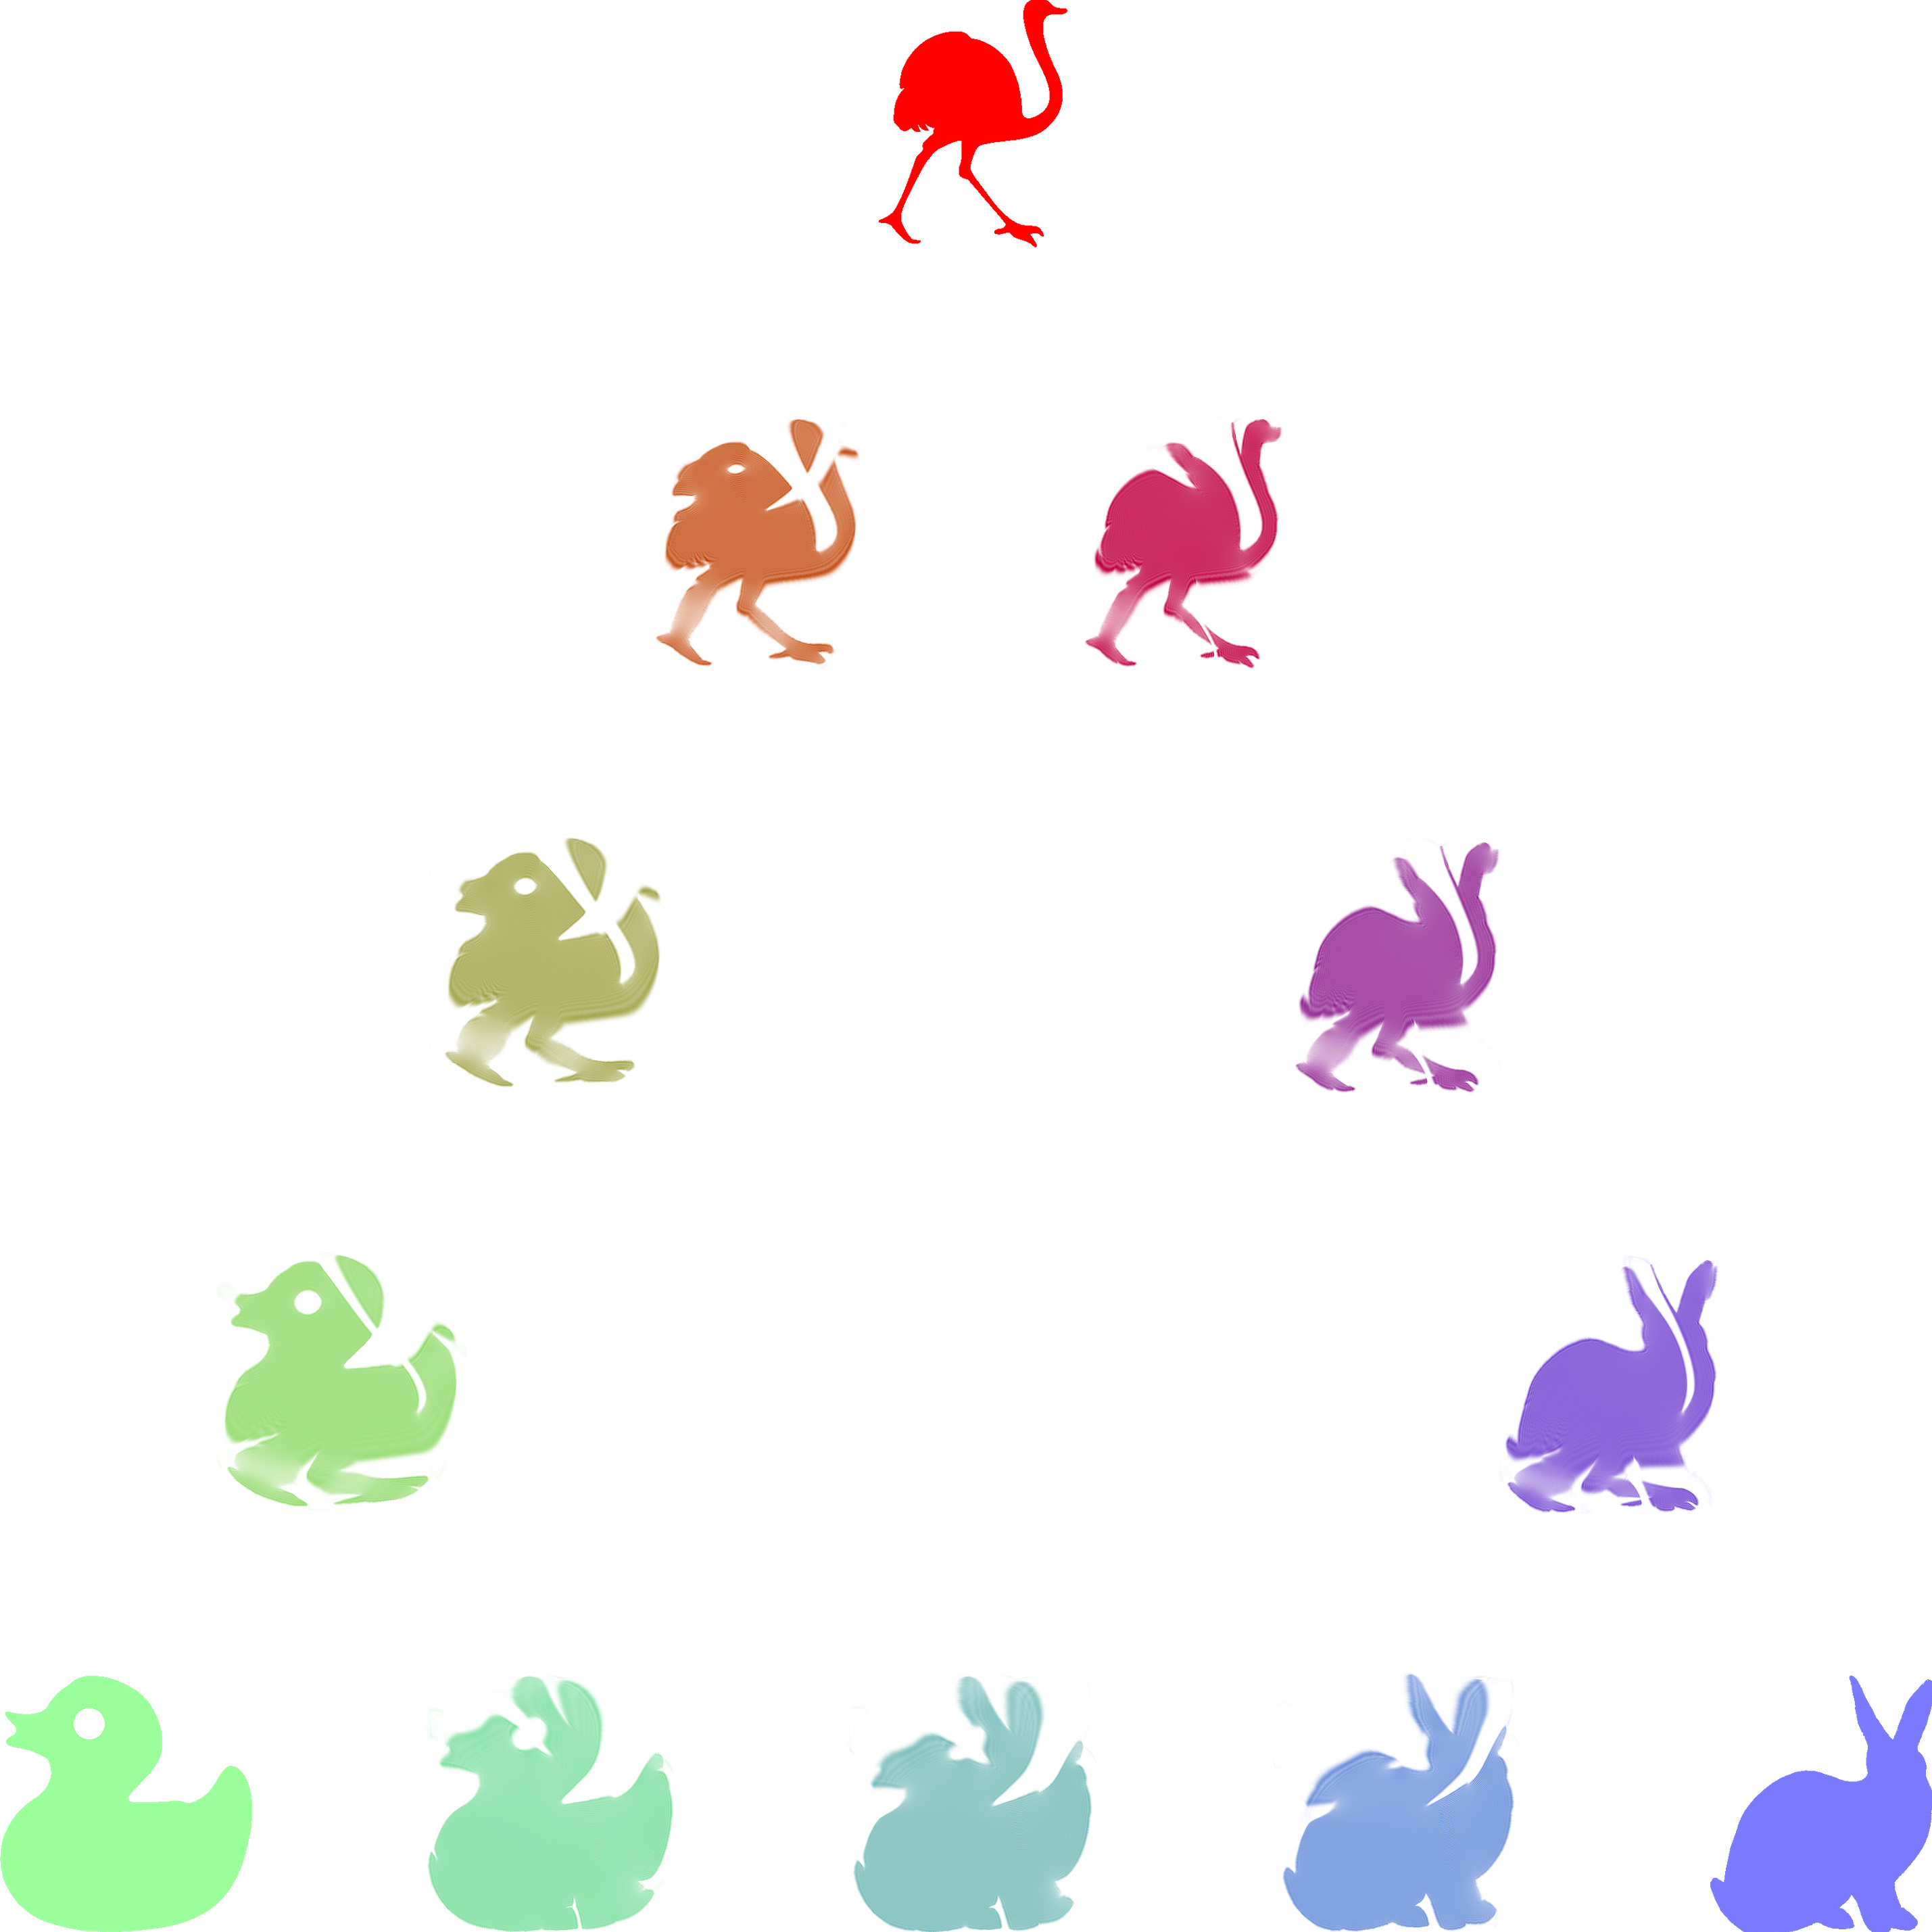
\includegraphics[width=0.31\linewidth]{animals/animalsColorRef} \\
 Radon barycenter  & Sliced barycenter & Wasserstein barycenter 
% & (b) Radon baryc. (Fast Slant Stack)
\end{tabular}
\end{center}
\caption{Comparison of $\Bary{\RR^d}^R, \Bary{\RR^d}^S$ and $\Bary{\RR^d}^W$ (computed using the method detailed in~\cite{FPapPeyOud13}).
}
\label{fig:compareRef}
\end{figure*}


%%%
\paragraph{Comparison of the Sliced and Radon barycenters.} 

As emphasized by Proposition~\ref{prop-comparison-bary}, while $\Bary{\RR^d}^R$ and $\Bary{\RR^d}^S$ are mathematically different, this difference is rather small, and is solely due to the lack of surjectivity of the Radon transform. We numerically evaluated this difference by computing 
\eq{
	\norm{ R(\Bary{\RR^d}^R(\mu_i, \lambda_i)_{i \in I}) - 
	\Bary{\Om^d}^W(R(\mu_i), \lambda_i)_{i \in I} }_{\text{TV}},
}
where $\norm{\cdot}_{\text{TV}}$ is the total variation of the measure defined in~\eqref{eq-tv-norm} and corresponds to the $L^1$ norm of the density in the case of an absolutely continuous measure. 
This measures the relative error due to the lack of surjectivity of $R$. Among several sets of discretized measures $\mu_i$ and weights $\lambda_i$, this relative error remained at approximately 0.15\%.
This said, the main difference between the sliced and Radon barycenter lies in their discretizations: $\Bary{\RR^d}^R$ is approximated with an Eulerian scheme and $\Bary{\RR^d}^S$ with a Lagrangian scheme.

\begin{figure}[!t]
\begin{center}
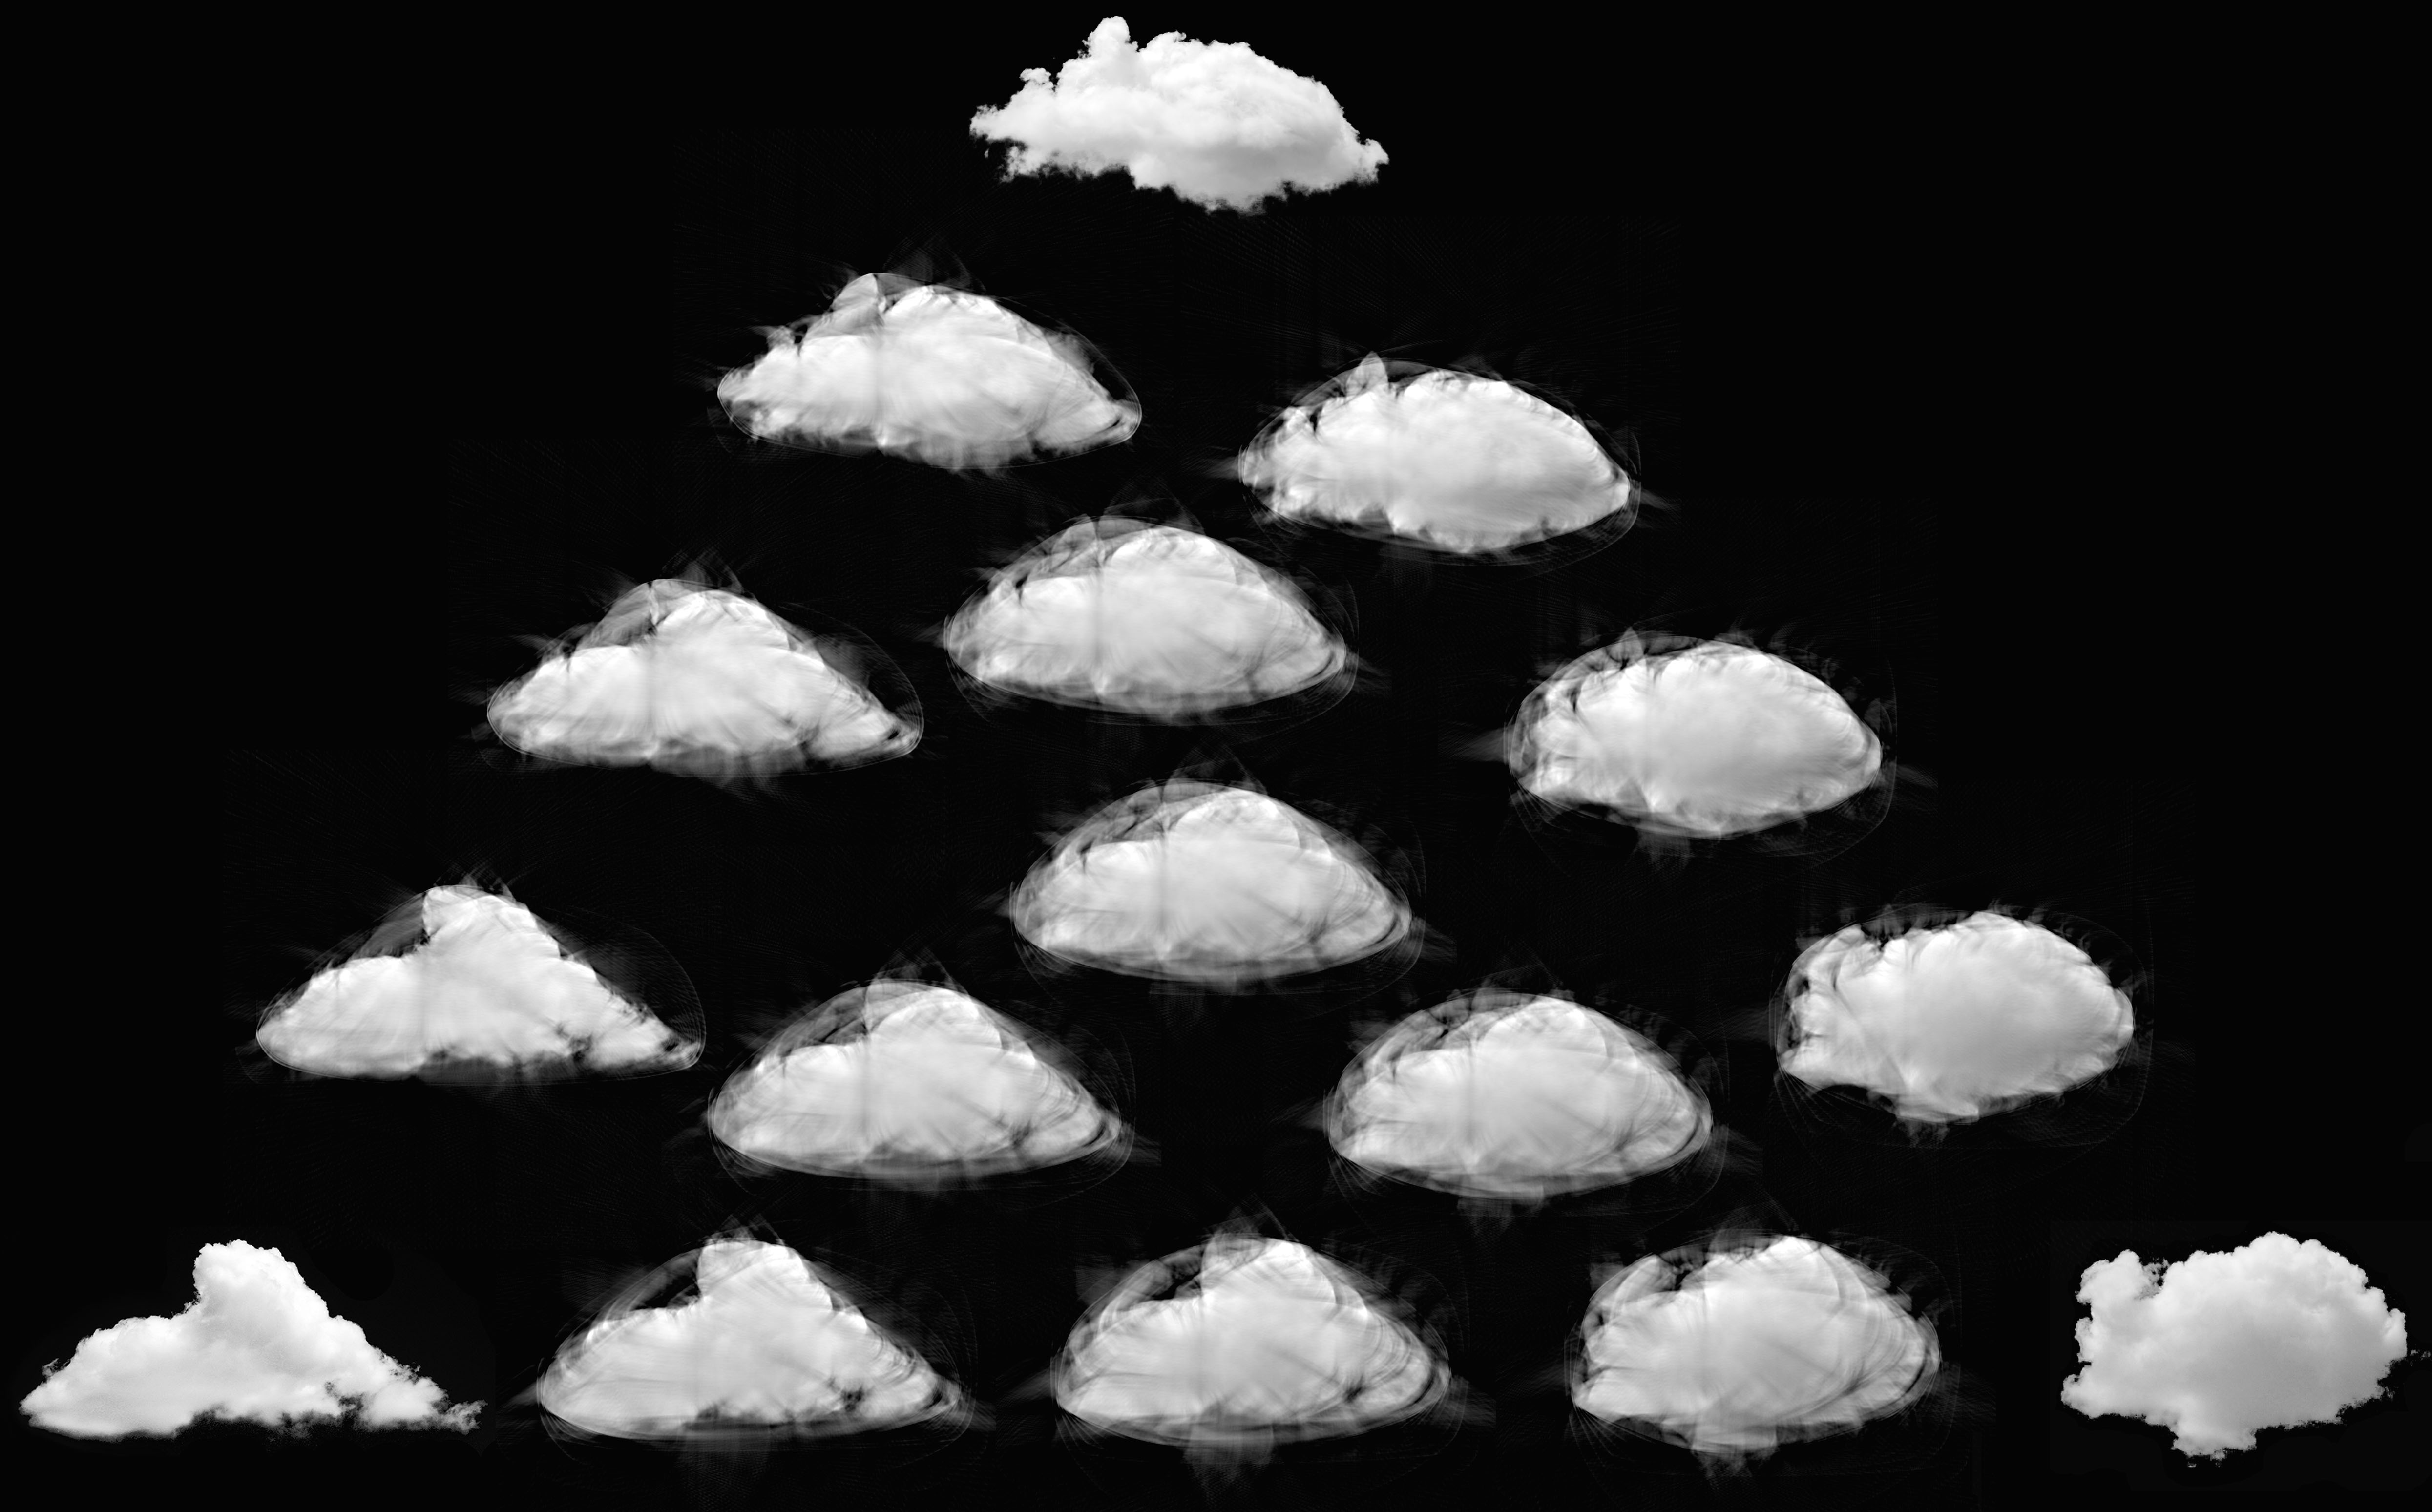
\includegraphics[width=\linewidth]{clouds/clouds.jpg}
\end{center}
\caption{Image warping using the Radon barycenter exhibits artifacts.  }
\label{fig:cloud}
\end{figure}


Figure~\ref{fig:compareRef} shows that the discretized barycenters are quite similar when computing the barycenter of three measures. Figure~\ref{fig:bary4} shows a similar comparison for the iso-barycenter of four measures. Figure~\ref{fig:cloud} shows what could be considered as a failure of the method to adapt to the computation of complex image barycenters. 

\begin{figure}[!t]
\begin{center}

\includegraphics[width=0.48\linewidth]{bary4/bary4_padded}

\includegraphics[width=0.48\linewidth]{bary4/bary4_SW2_100dir_40kpoints_sig20_N512pix}
\end{center}
\caption{Top: Radon barycenter $\Bary{\RR^d}^R$ of four 2-D distributions with equal weights. 
Bottom : Same experiment with SW2, using $N=4\,10^4$ points samples, $|\Theta|=100$ directions and a gaussian kernel with standard deviation $\sigma=20/512$ to estimate the corresponding densities. .
}
\label{fig:bary4}
\end{figure}


%%%
\paragraph{Comparison of computational complexity.}

A typical Radon barycenter of three two-dimensional pdfs discretized on a $1024 \times 1024$ pixel grid, and the principled Fast Slant Stack Radon transform with $2048$ slices, requires $11$ seconds to precompute the initial Radon transforms, and $170$ seconds to compute $32$ Radon barycenters, with unoptimized parallel Matlab code. It is possible to accelerate this timing using less precise Radon transform. For instance, using Matlab's implementation of the Radon transform with $180$ slices requires $14$ seconds to compute these $32$ barycenters on a single core. 
In comparison with the Eulerian proximal splitting method of Papadakis et al.~\cite{FPapPeyOud13}, the Wasserstein barycenter between two $1024 \times 1024$ distributions with $32$ time steps and $100,000$ iterations to achieve an acceptable convergence requires on average 72 hours, using an optimized C++ vectorized and parallel implementation (see Fig.~\ref{fig:compareRef} for a display of the resulting barycenters).

A sliced barycenter of three distributions, each approximated with 40k Dirac masses and 100 directions, requires 140 seconds using 100 iterations of Newton descent or 18 seconds using the stochastic Newton descent with subsets of 10 directions. With a finer set of 1000 directions and the same setup, the stochastic Newton descent with subsets of 100 directions requires 168 seconds.


%%%
\paragraph{Comparison with the entropy regularized barycenter~\cite{CuturiBarycenter}.}

Cuturi and Doucet proposed in~\cite{CuturiBarycenter} a method to approximate the Wasserstein barycenter on a fixed grid, hence using the Eulerian discretization presented in Section~\ref{subsec-algorithm-eulerian}. Their method performs a gradient descent on a smoothed Wasserstein distance. This smoothing is obtained by adding an entropic penalization to the linear cost function~\eqref{eq-dfn-wass-dist} defining the transportation distance. Figure~\ref{fig:compareMarco} shows a visual comparison of the iso-barycenters computed with this approach as well as with the sliced and Radon methods. 

The result obtained with the method of~\cite{CuturiBarycenter} is produced in two hours on a GPU, using a $150 \times 150$ sampling grid. In contrast, our Radon barycenter computed on a grid of $400 \times 400$ pixels (which is zero-padded to $1200 \times 1200$ pixels to avoid Radon transform artifacts) is obtained in 40 seconds using the fast slant stack approach with 1200 directions, and 2 seconds with Matlab built-in Radon transforms with 180 directions, on a single core of a laptop. Similarly, our Sliced barycenter implemented in Matlab produced the interpolation in 20 minutes, using $4 \times 10^5$ points sampled on a interpolated grid of $1000 \times 1000$ pixels, with 100 directions and 100 iterations.

\begin{figure}[!ht]
\begin{center} 
\begin{tabular}{c@{\hspace{1mm}}c@{\hspace{1mm}}c@{}}
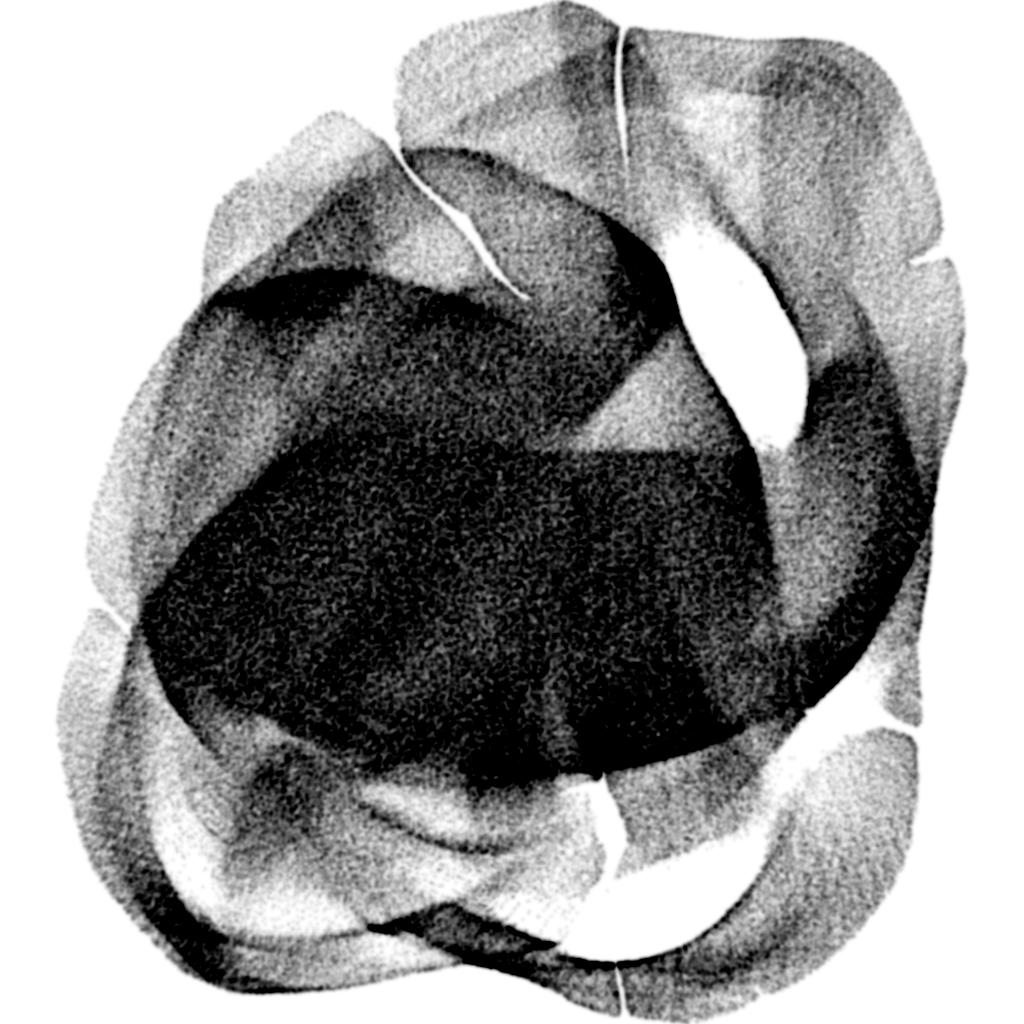
\includegraphics[width=.32\linewidth]{cuturi/bary-animals-Sliced-1-1-1_thresh} &
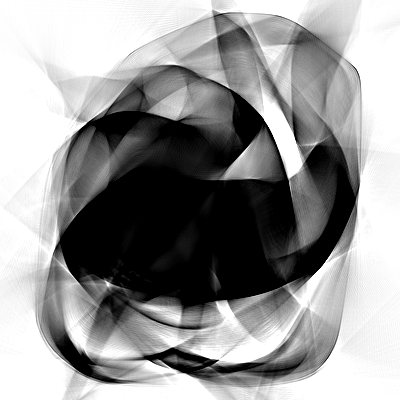
\includegraphics[width=.32\linewidth]{cuturi/animal_padded111} &

\includegraphics[width=.32\linewidth]{cuturi/bary-animals-cuturi-1-1-1} \\
$\Bary{\RR^d}^S$ & $\Bary{\RR^d}^R$ & Cuturi et al.
\end{tabular}
\end{center}
\caption{Comparison of three methods (Sliced, Radon, and the one presented in~\cite{CuturiBarycenter}) to compute isobarycenters (i.e. using $\la=(1,1,1)/3$) of the three input densities displayed at the vertices of Figure~\ref{fig:compareRef}, bottom. 
}
\label{fig:compareMarco}
\end{figure}


%%%%%%%%%%%%%%%%%%%%%%%%%%%%%%%%%%%%%%%%%%%%%%%%%%%
\subsection{Application to Texture Mixing} 

To illustrate the usefulness of the Radon barycenter, we apply it to the problem of texture mixing. The Radon barycenter is well suited to this application which requires an Eulerian discretization in order to interpolate power-spectra computed on the uniform grid of Fourier frequencies. This would be hardly feasible using the Lagrangian discretization of the Sliced barycenter. 


%%%%%
\paragraph{Texture mixing.}

Given a set of input texture images $\{ f^{[i]} \}_{i \in I}$, where each $f^{[i]} \in \RR^N$ is a grayscale image of $N=n \times n$ pixels, the goal of texture mixing is to produce a set of random vectors $\{ F^{[i]} \}_{i \in I}$, and an interpolation method $\la \in \La_I \mapsto F_\la$. In particular, it means that if $\la$ is $0$ excepted at the $i^{\text{th}}$ coordinate, then $F_\la=F^{[i]}$ (interpolation at the vertices of the simplex indexed by $I$). Texture mixing is a generalization of texture synthesis (which simply corresponds to the case $|I|=1$), in the sense that any realization $\tilde f^{[i]}$ of the random vector $F^{[i]}$ should look both ``random'' and visually similar (but not equal) to the input $f^{[i]}$.


%%%%%
\paragraph{Spot-noise (SN) texture model.}

Following the work of~\cite{galerne-ieee} (which introduces the name ``spot noise'' model), we consider stationary Gaussian random vectors $F$ which take values in $\RR^N$. These vectors are indexed on the image grid 
\eq{
	F = (F_k)_{k \in \Gg}
	\qwhereq
	\Gg = \{-n/2+1, \ldots, n/2\}^2, 
}
(for simplicity we assume that $n$ is even) and we use periodic boundary conditions. Without loss of generality, we assume that they have zero mean $\EE(F)=0$. 
% and unit global variance $\EE(\norm{F}^2)=1$. Note the mean and the variance are usually adjusted to match the contrast of the display. 
Such a random vector is thus entirely characterized by its (square root) power spectrum density (PSD)
\eq{
	\foralls \om \in \Gg, \quad P_F(\om) = \EE( |\hat F(\om)|^2 )^{1/2} 
}
where we define the Fourier transform of a vector or a random vector as
\eq{
	\foralls \om \in \Gg, \quad
	\hat F(\om) = \sum_{k \in \Gg} F_k e^{\frac{2 \imath \pi}{n} \dotp{k}{\om} }
}
\eq{
	\qwhereq
	 \dotp{k}{\om} = k_1 \om_1 + k_2 \om_2.
} 
We remind that once the power-spectrum $P_F$ of $F$ is known, $F$ is recovered by 
\eql{\label{eq-gaussian-sampling}
	\hat F(\om) = P_F(\om) \cdot \hat W(\om)
	\qwhereq
	W \sim \Nn(0,\Id_{N}).
}
It is thus easy to draw a realization $f$ of the vector $F$ by convolving the inverse Fourier transform of $P_F$ (the so-called texton, see~\cite{Desolneux-Moisan-12}) by a realization $w$ of the white noise $W$, i.e., computing $\hat f = P_F \cdot \hat w$, where $\cdot$ denotes entry-wise multiplication.


In this spot noise model, it is customary (see~\cite{galerne-ieee}) to learn the input Gaussian models $\{F^{[i]}\}_{i \in I}$ by estimating their PSD with a maximum likelihood estimation, which corresponds to estimating the covariance using the empirical periodogram
\eq{
	\foralls i \in I, \quad \foralls \om \in \Gg, \quad
	P_{F^{[i]}}(\om) = |\hat f^{[i]}(\om)|. 
} 
We also use this estimation, which, despite its simplicity, gives good visual performances, see~\cite{peyre2013Gaussians}. 

%%%%%
\paragraph{Optimal transport barycenter of SN models.}

We introduce a texture mixing method that performs the interpolation of the PSD using optimal transport. The rational of this method is to operate the mixing with geometric warpings of the spectral modes of the textures. The method is thus adapted to deal with micro-textures which exhibit a high degree of sparsity in the Fourier domain, i.e., which PSD are composed of a few localized spikes. This class of sparse spectral textures has been shown in~\cite{GalerneGabor} to be a powerful way to approximate more complicated textures for procedural texture synthesis. 

We define the measure associated to the PSD of the Gaussian model $F^{[i]}$ 
\eq{
	\foralls i \in I, \quad
	\mu_i = \frac{1}{\sum_{\om \in \Gg} P_{F^{[i]}}(\om)} 
		\sum_{\om \in \Gg} P_{F^{[i]}}(\om) \de_{\om} \in \Mm_1^+(\RR^2).
}
The barycenter measure is defined as
\eq{
	\foralls \la \in \La_I, \quad
	\mu^{(\la)} = \Bary{\RR^2}^R( \mu_i, \la_i )_{i \in I}.
}
Note that this measure exhibits central symmetry because of~\eqref{eq-prop-inv-cent} and Proposition~\eqref{prop:InvarianceHolds}.

This barycenter measure is approximated using the Eulerian discretized Radon barycenter described in Section~\ref{subsec-algorithm-eulerian}, to obtain a resulting measure 
\eq{	
	\bar\mu^{(\la)} = \Bary{\Gg}^R( \mu_i, \la_i )_{i \in I}.
}
By construction of this algorithm, this measure is supported on the grid $\Gg$ and also exhibits central symmetry. It can thus be written as
\eq{
	\bar\mu^{(\la)} = \sum_{\om \in \Gg} P_{F_\la}(\om) \de_{\om}.
}
This thus defines a stationary Gaussian random vector $F_\la$ through its PSD $P_{F_\la}$. This Gaussian vector is our interpolated model, which can be synthesized following~\eqref{eq-gaussian-sampling}. 


%%%%%
\paragraph{Examples.} 

We demonstrate our Radon barycenter of power spectrum densities on several examples. A sparse hand-de\-si\-gned power spectrum is interpolated in Fig.~\ref{fig:texsynth} and a more natural, less sparse, power spectrum is used in Fig.~\ref{fig:texsynth2}.
We handle colors by convolving the interpolated power spectrum of each color channel by the same white noise. Although the decoupling of color channels could occasionally lead to color artifacts, we did not 
observe such effects on our set of examples (further examples can be see in the additional material). We hence leave the investigation of perceptually decoupled color spaces 
or the joint transportation of color channels for future work.
%\todo{Then it means you treat each channel independently and do barycenter for each channel ? I thought this would leads to color artifact since you do not model the cross correlation between the channels. This needs clarification. }.

%\todo{Detail a bit, in particular how to handle colors}


\begin{figure*}[!t]
\setlength{\tabcolsep}{0pt}
  \setlength{\fboxsep}{0pt}
\begin{center} 
\begin{tabular}{@{}c@{\hspace{1mm}}c@{}}
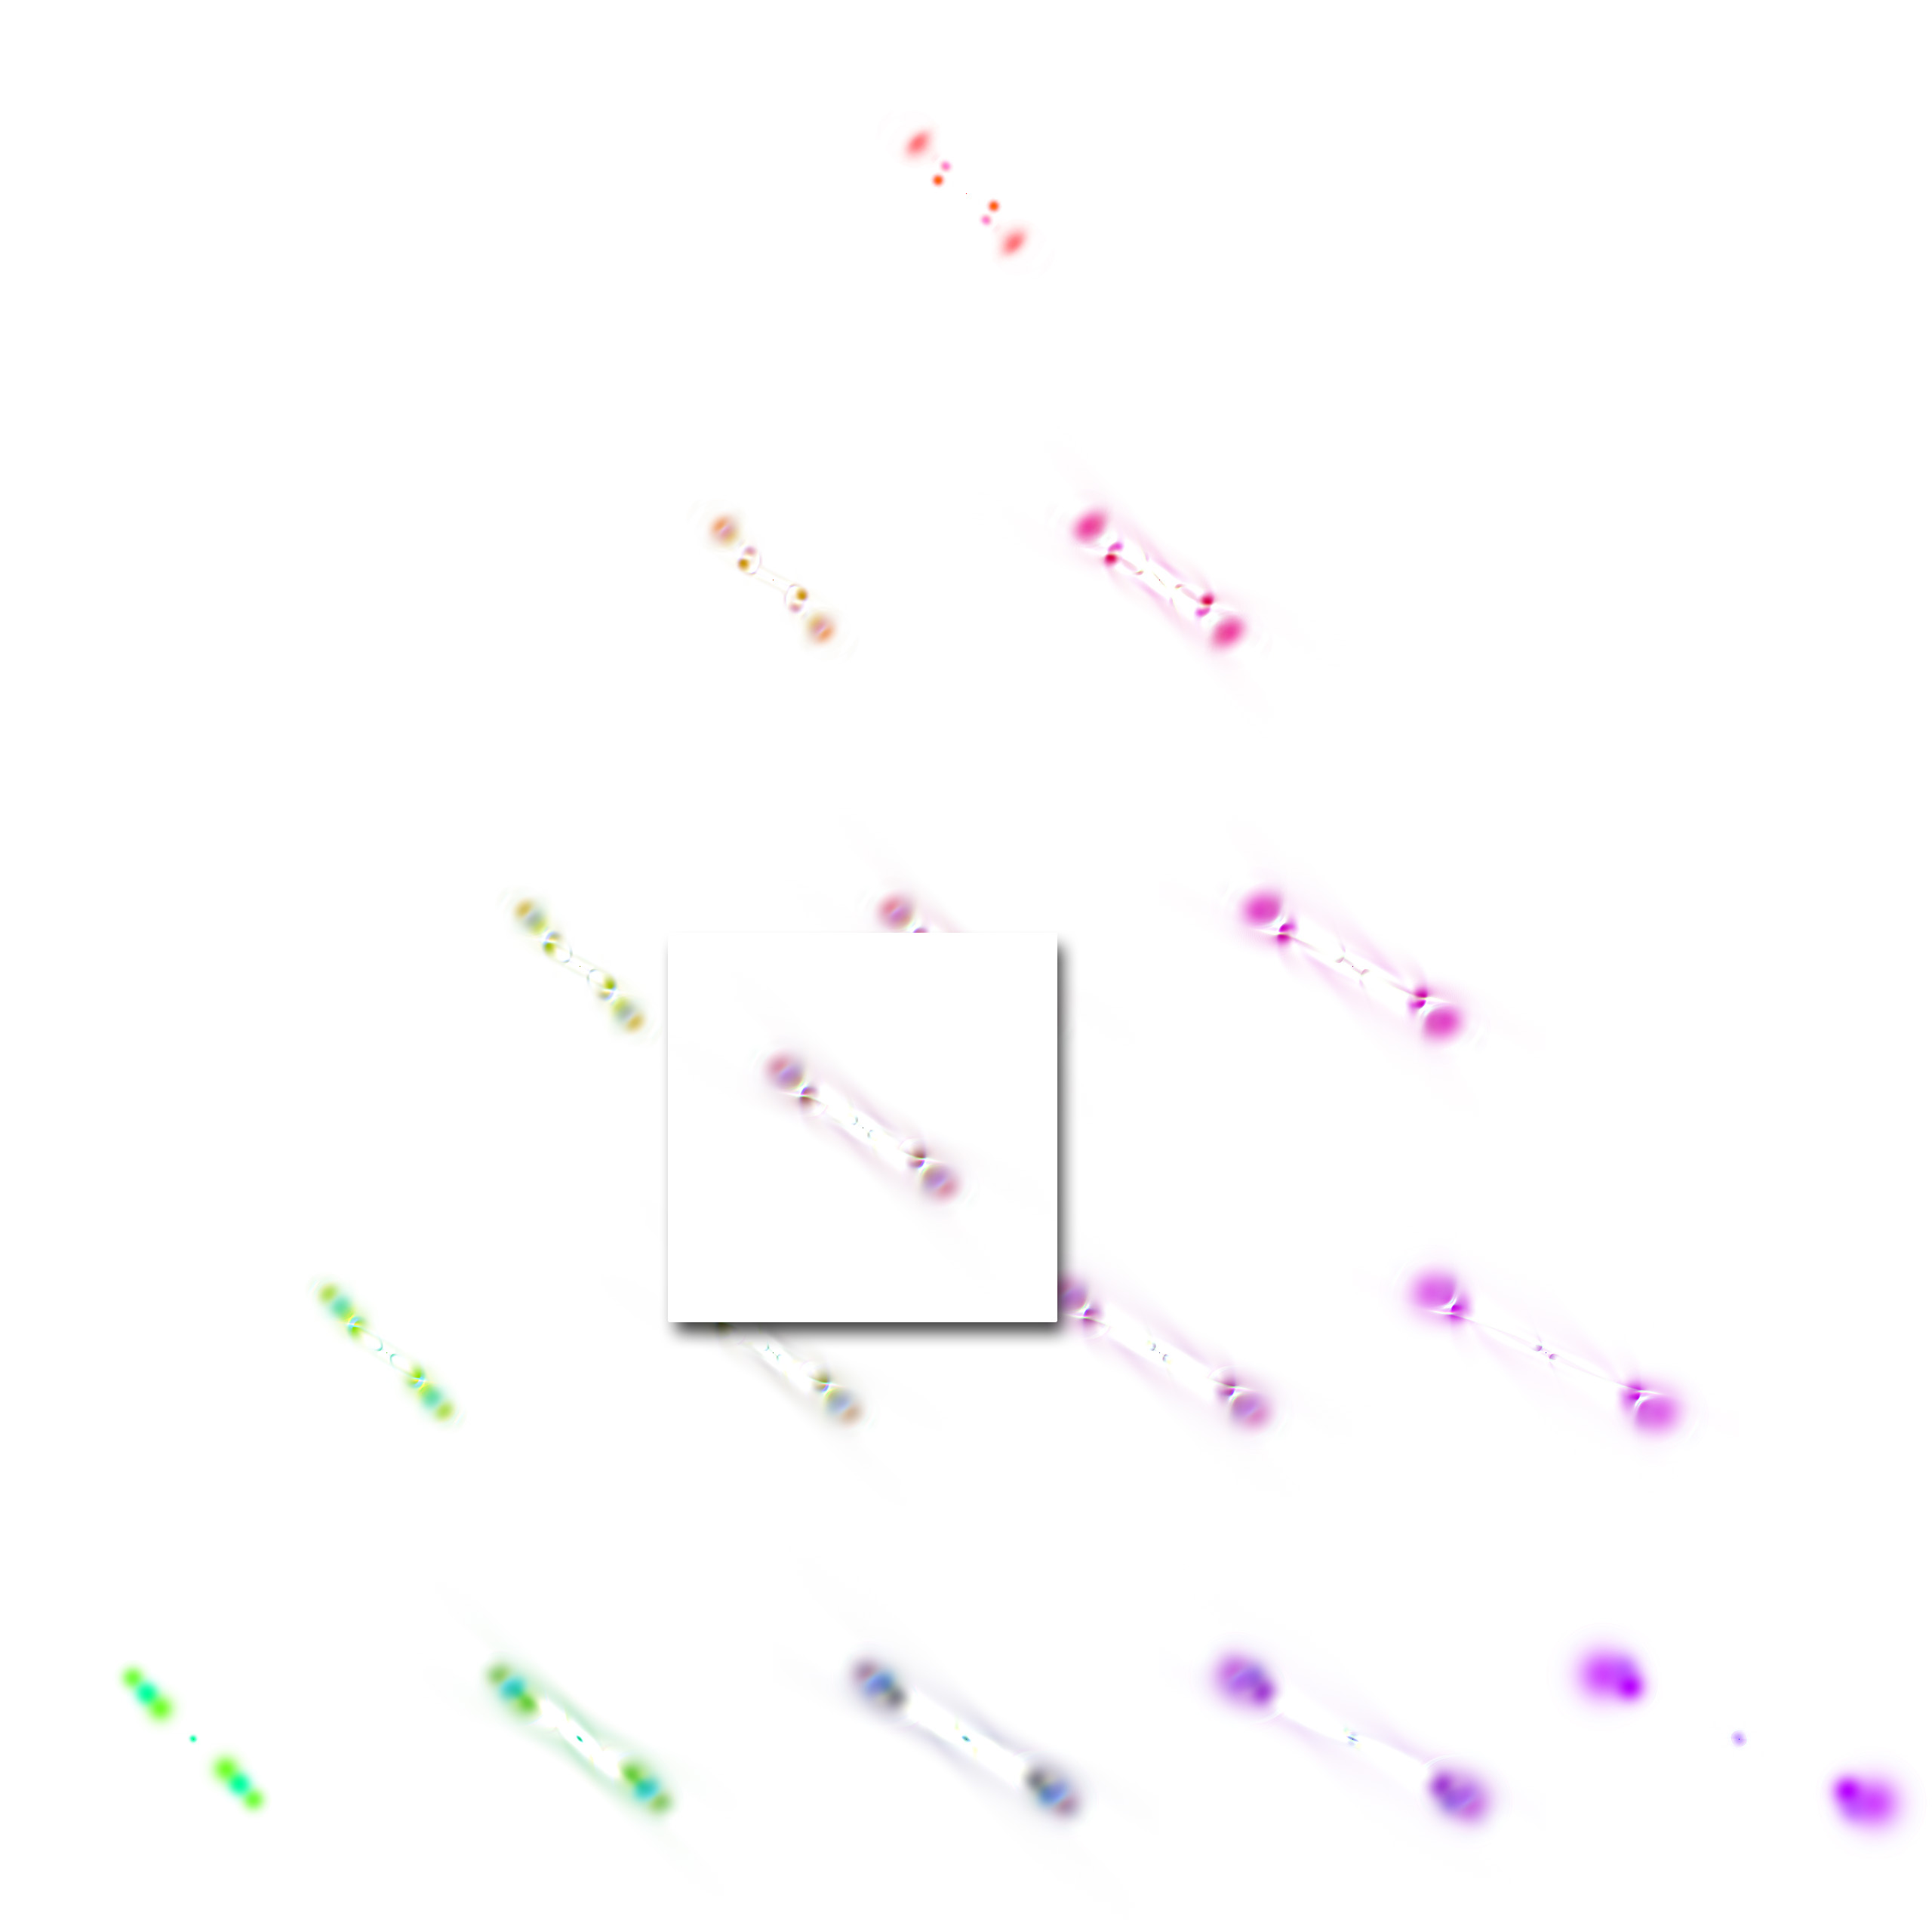
\includegraphics[width=0.3\linewidth]{textures/manCspec_fastslant} &
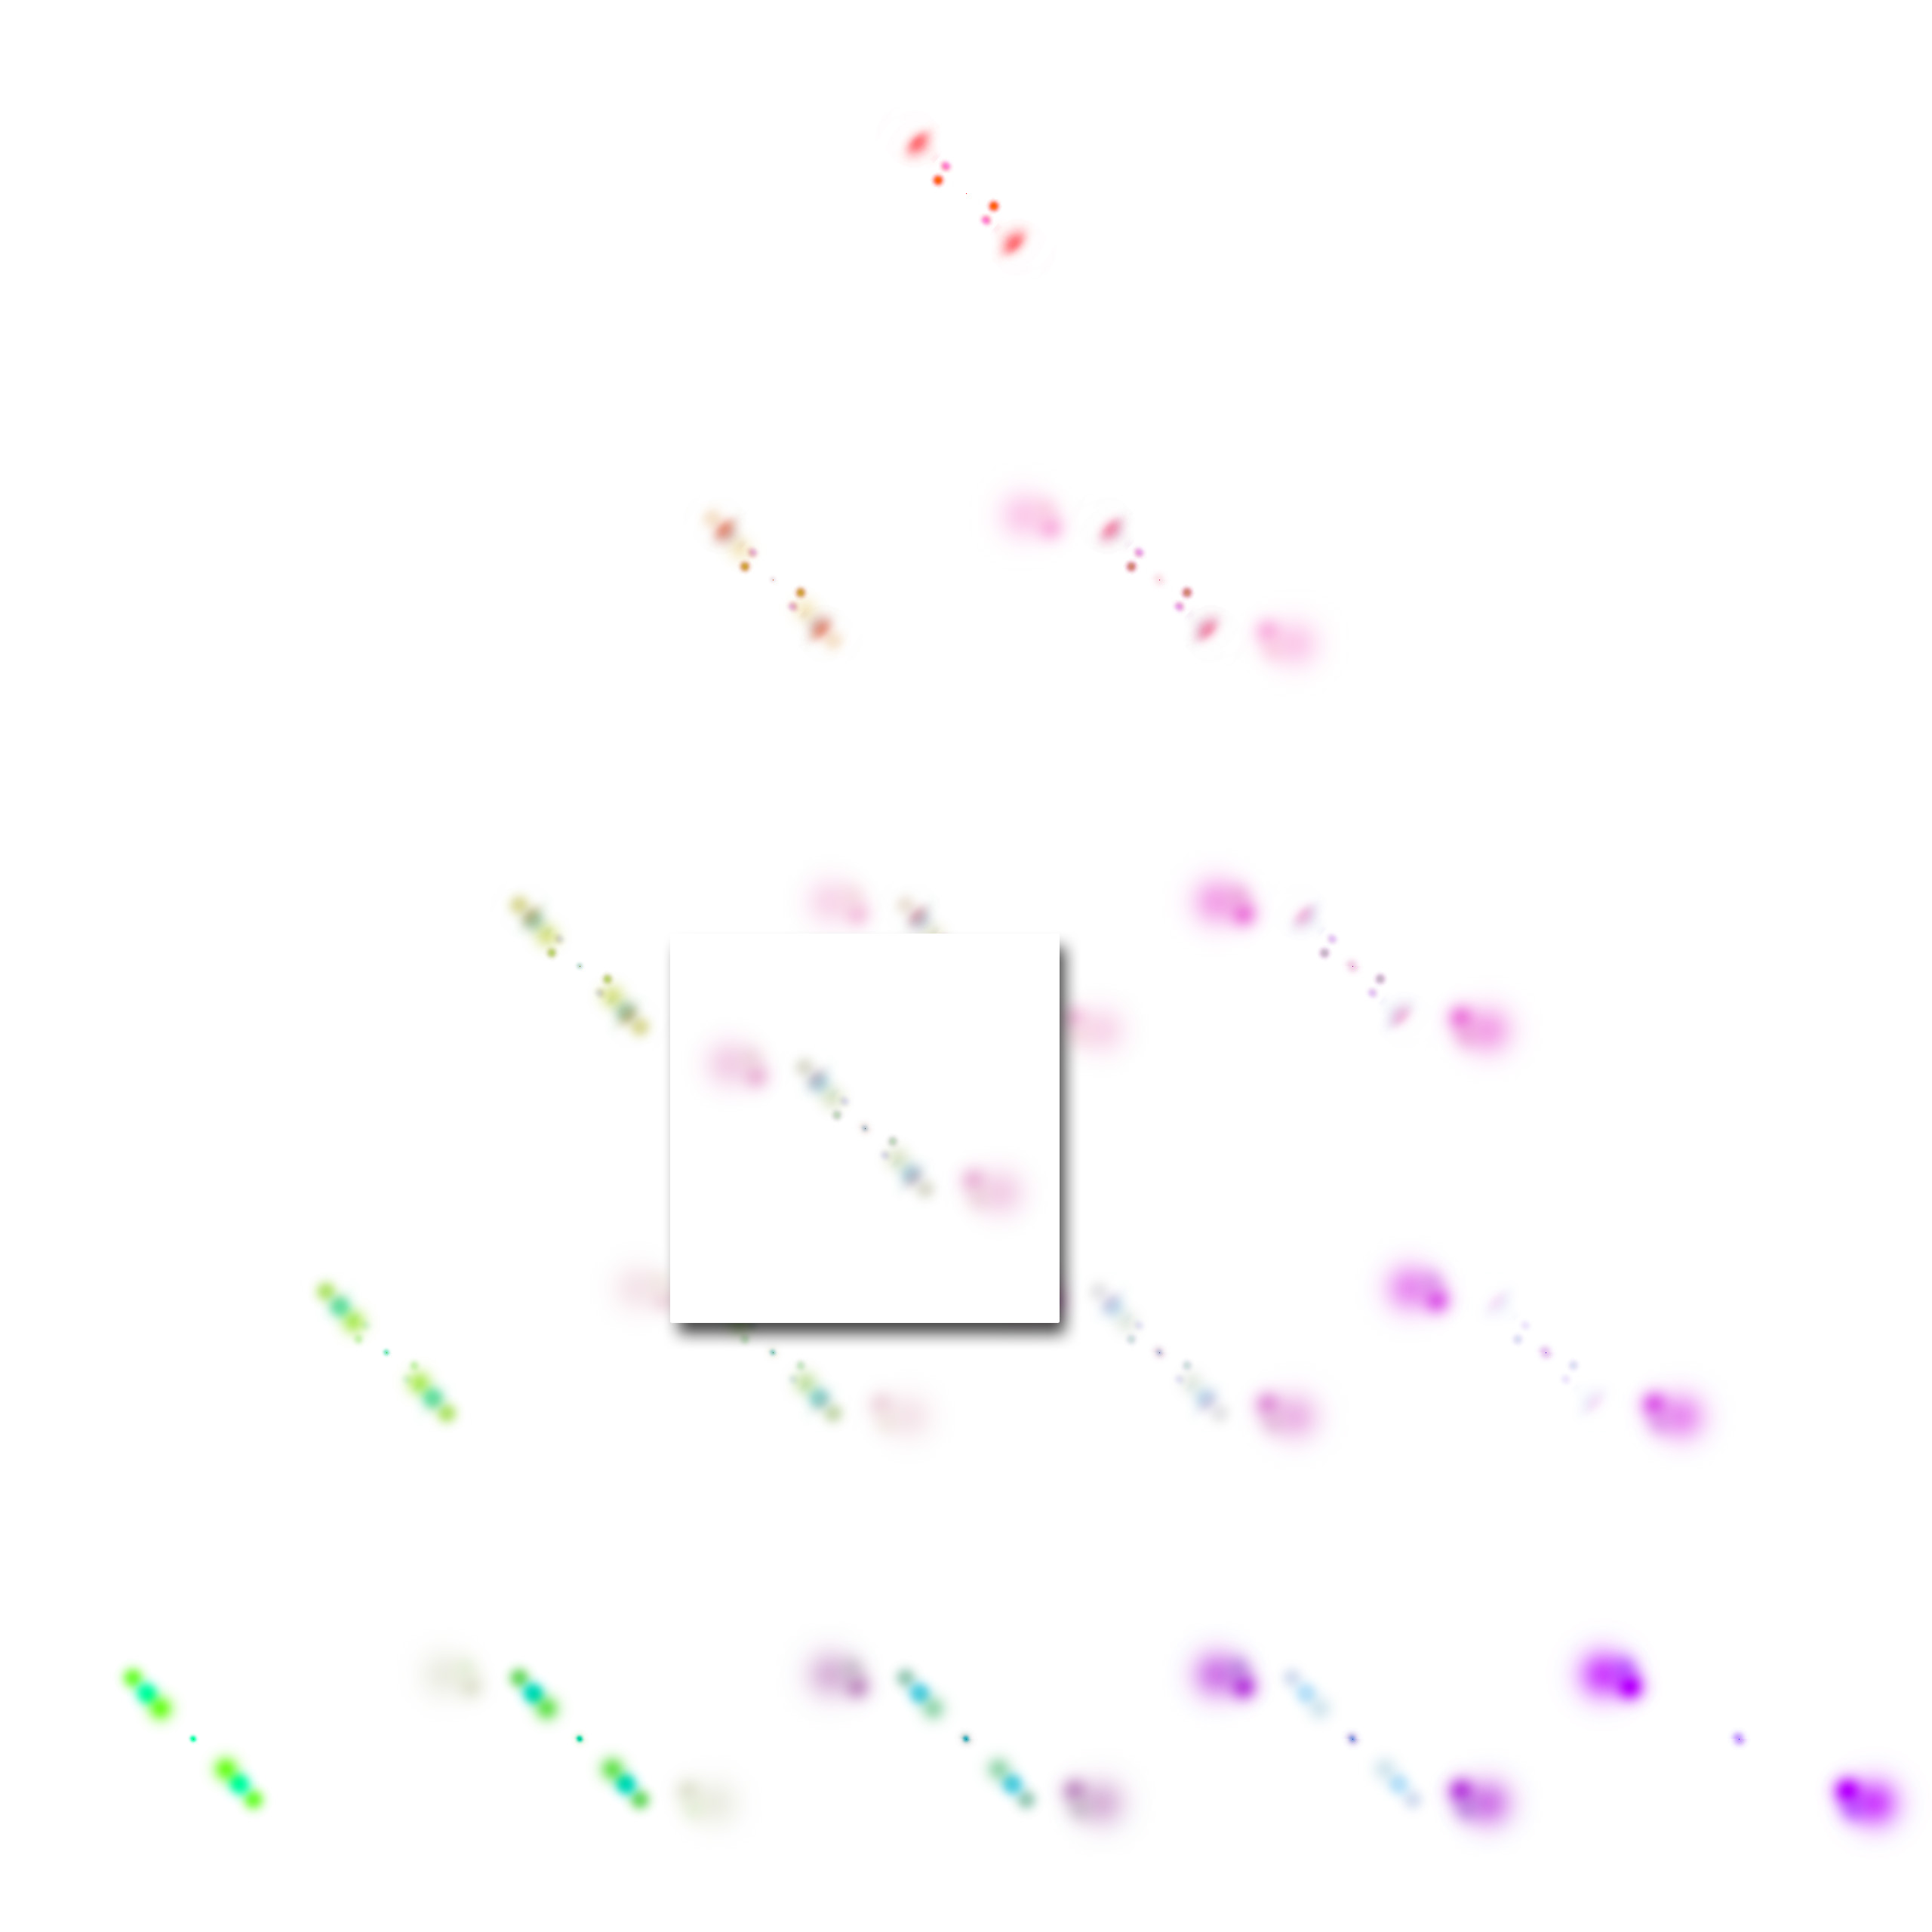
\includegraphics[width=0.3\linewidth]{textures/manCspec_Naive}  \\
 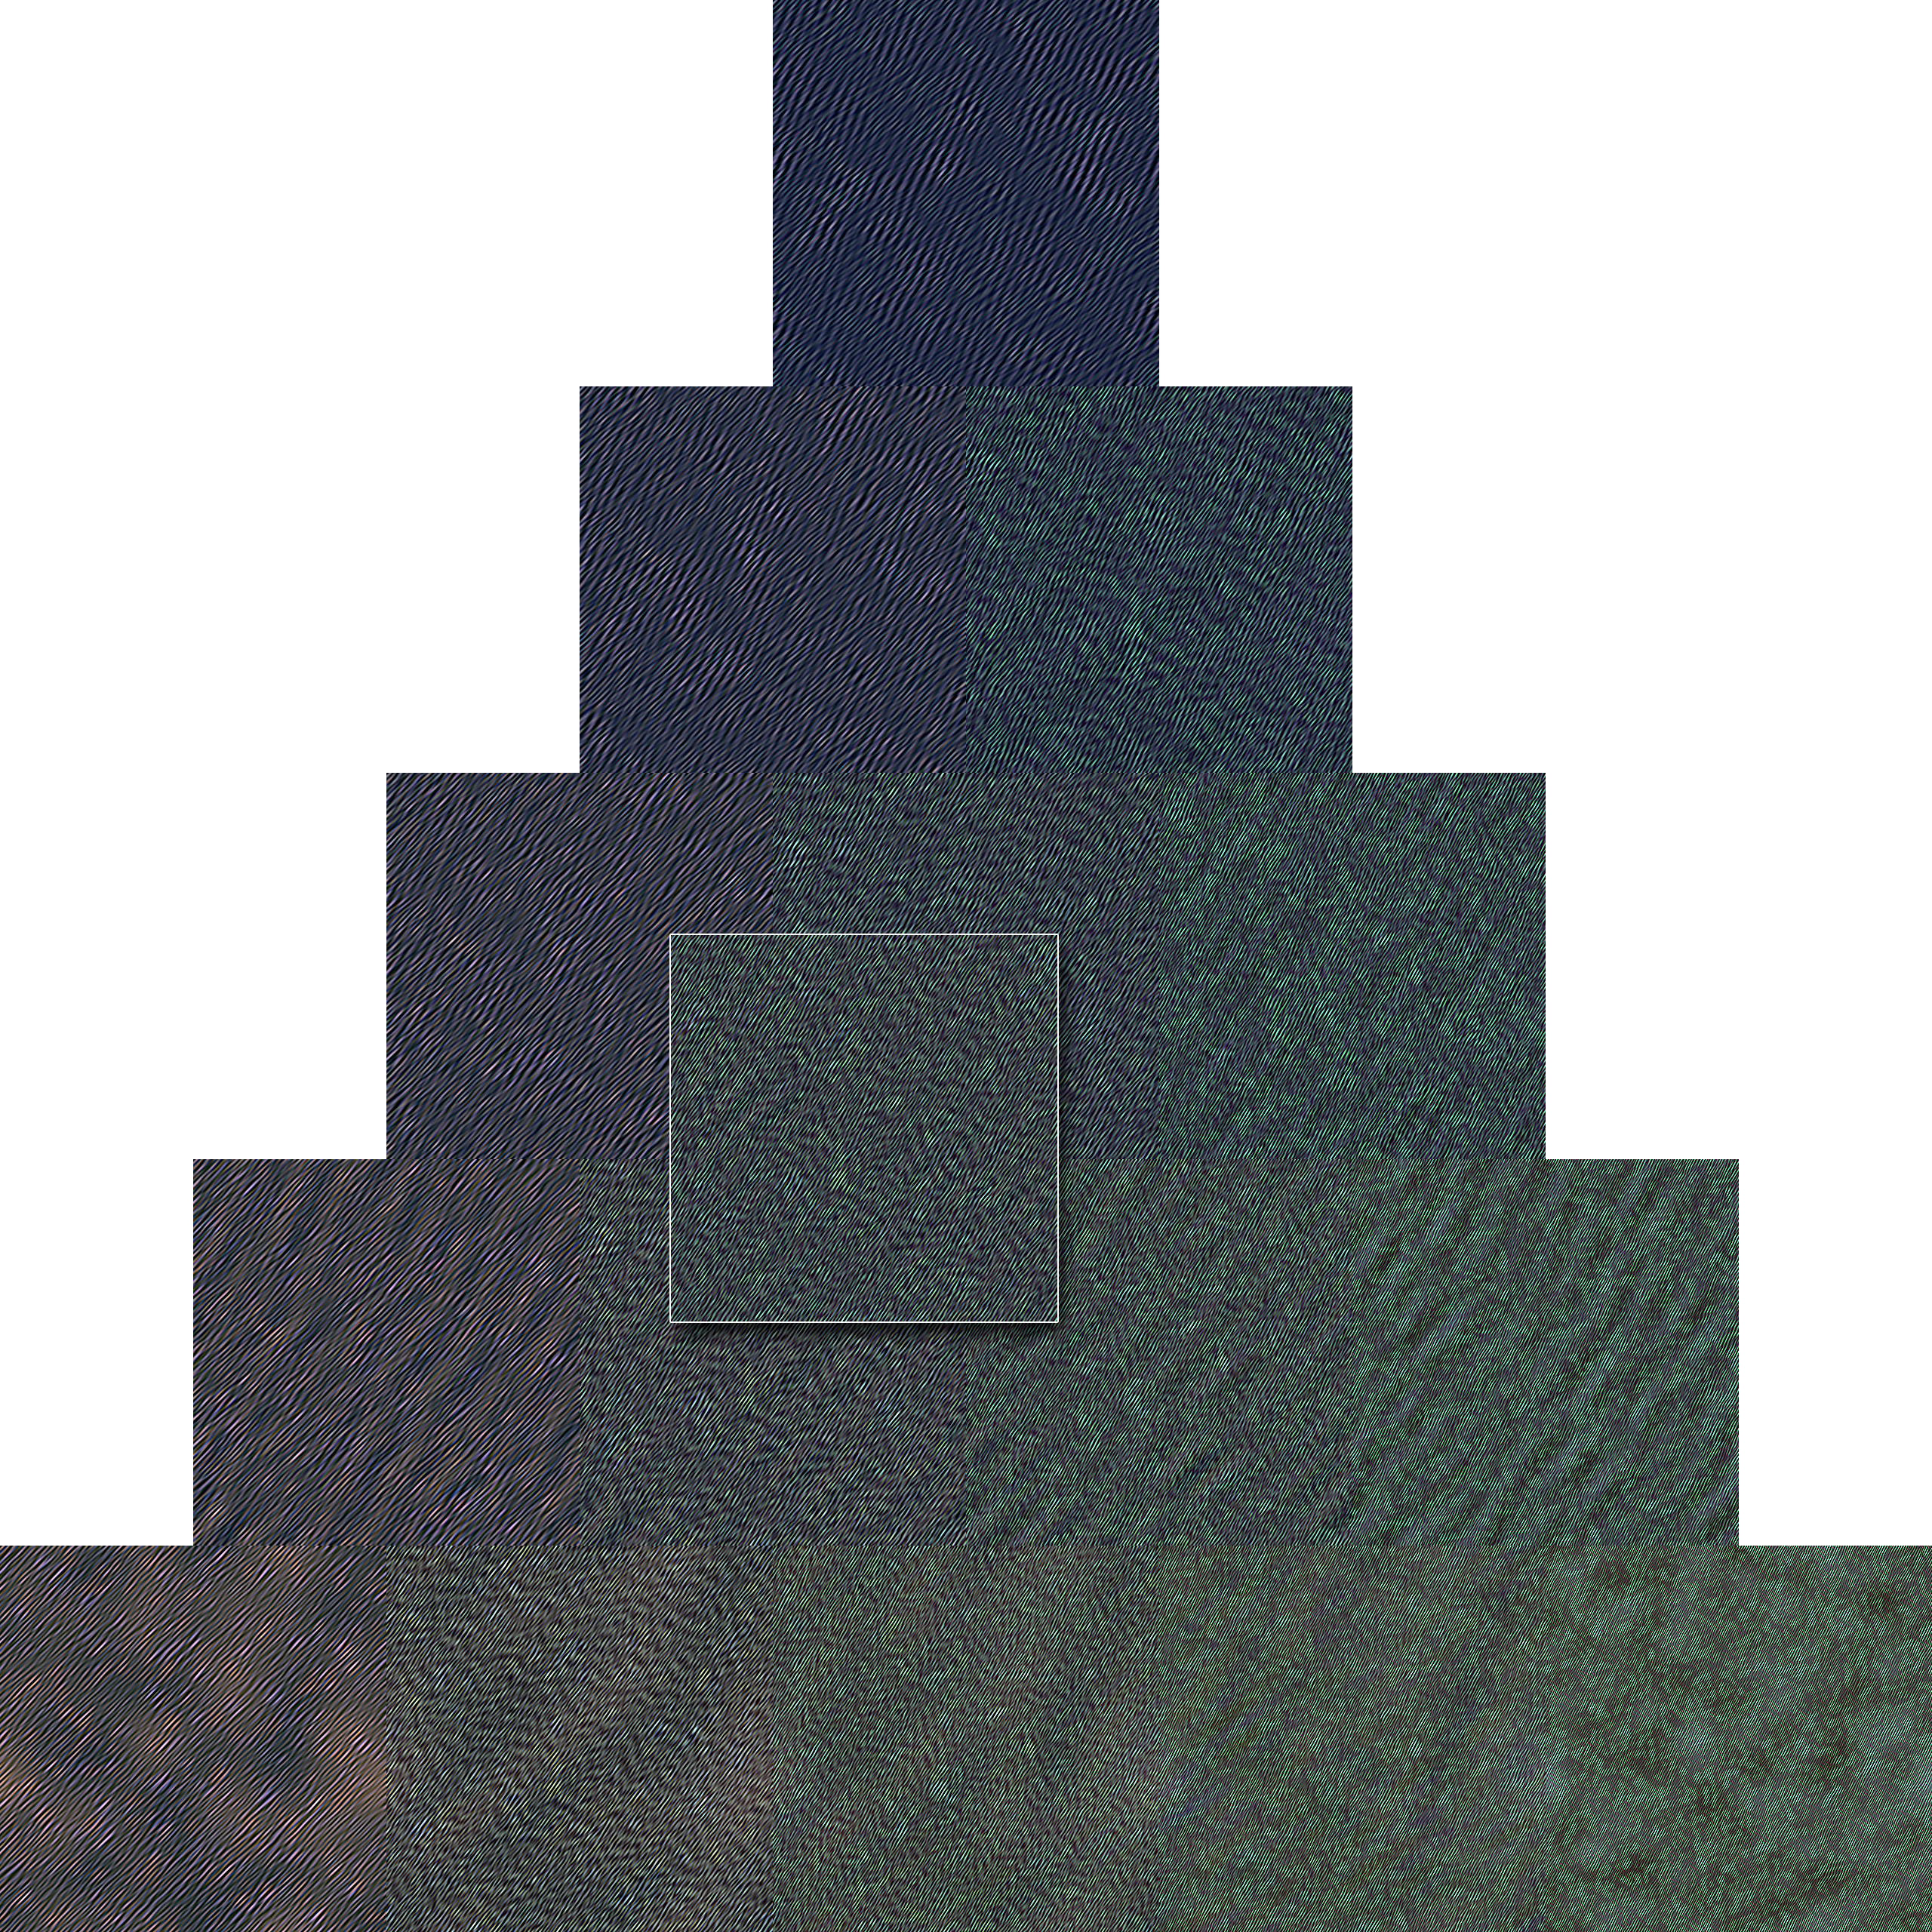
\includegraphics[width=0.49\linewidth]{textures/manC_fastslant}  &
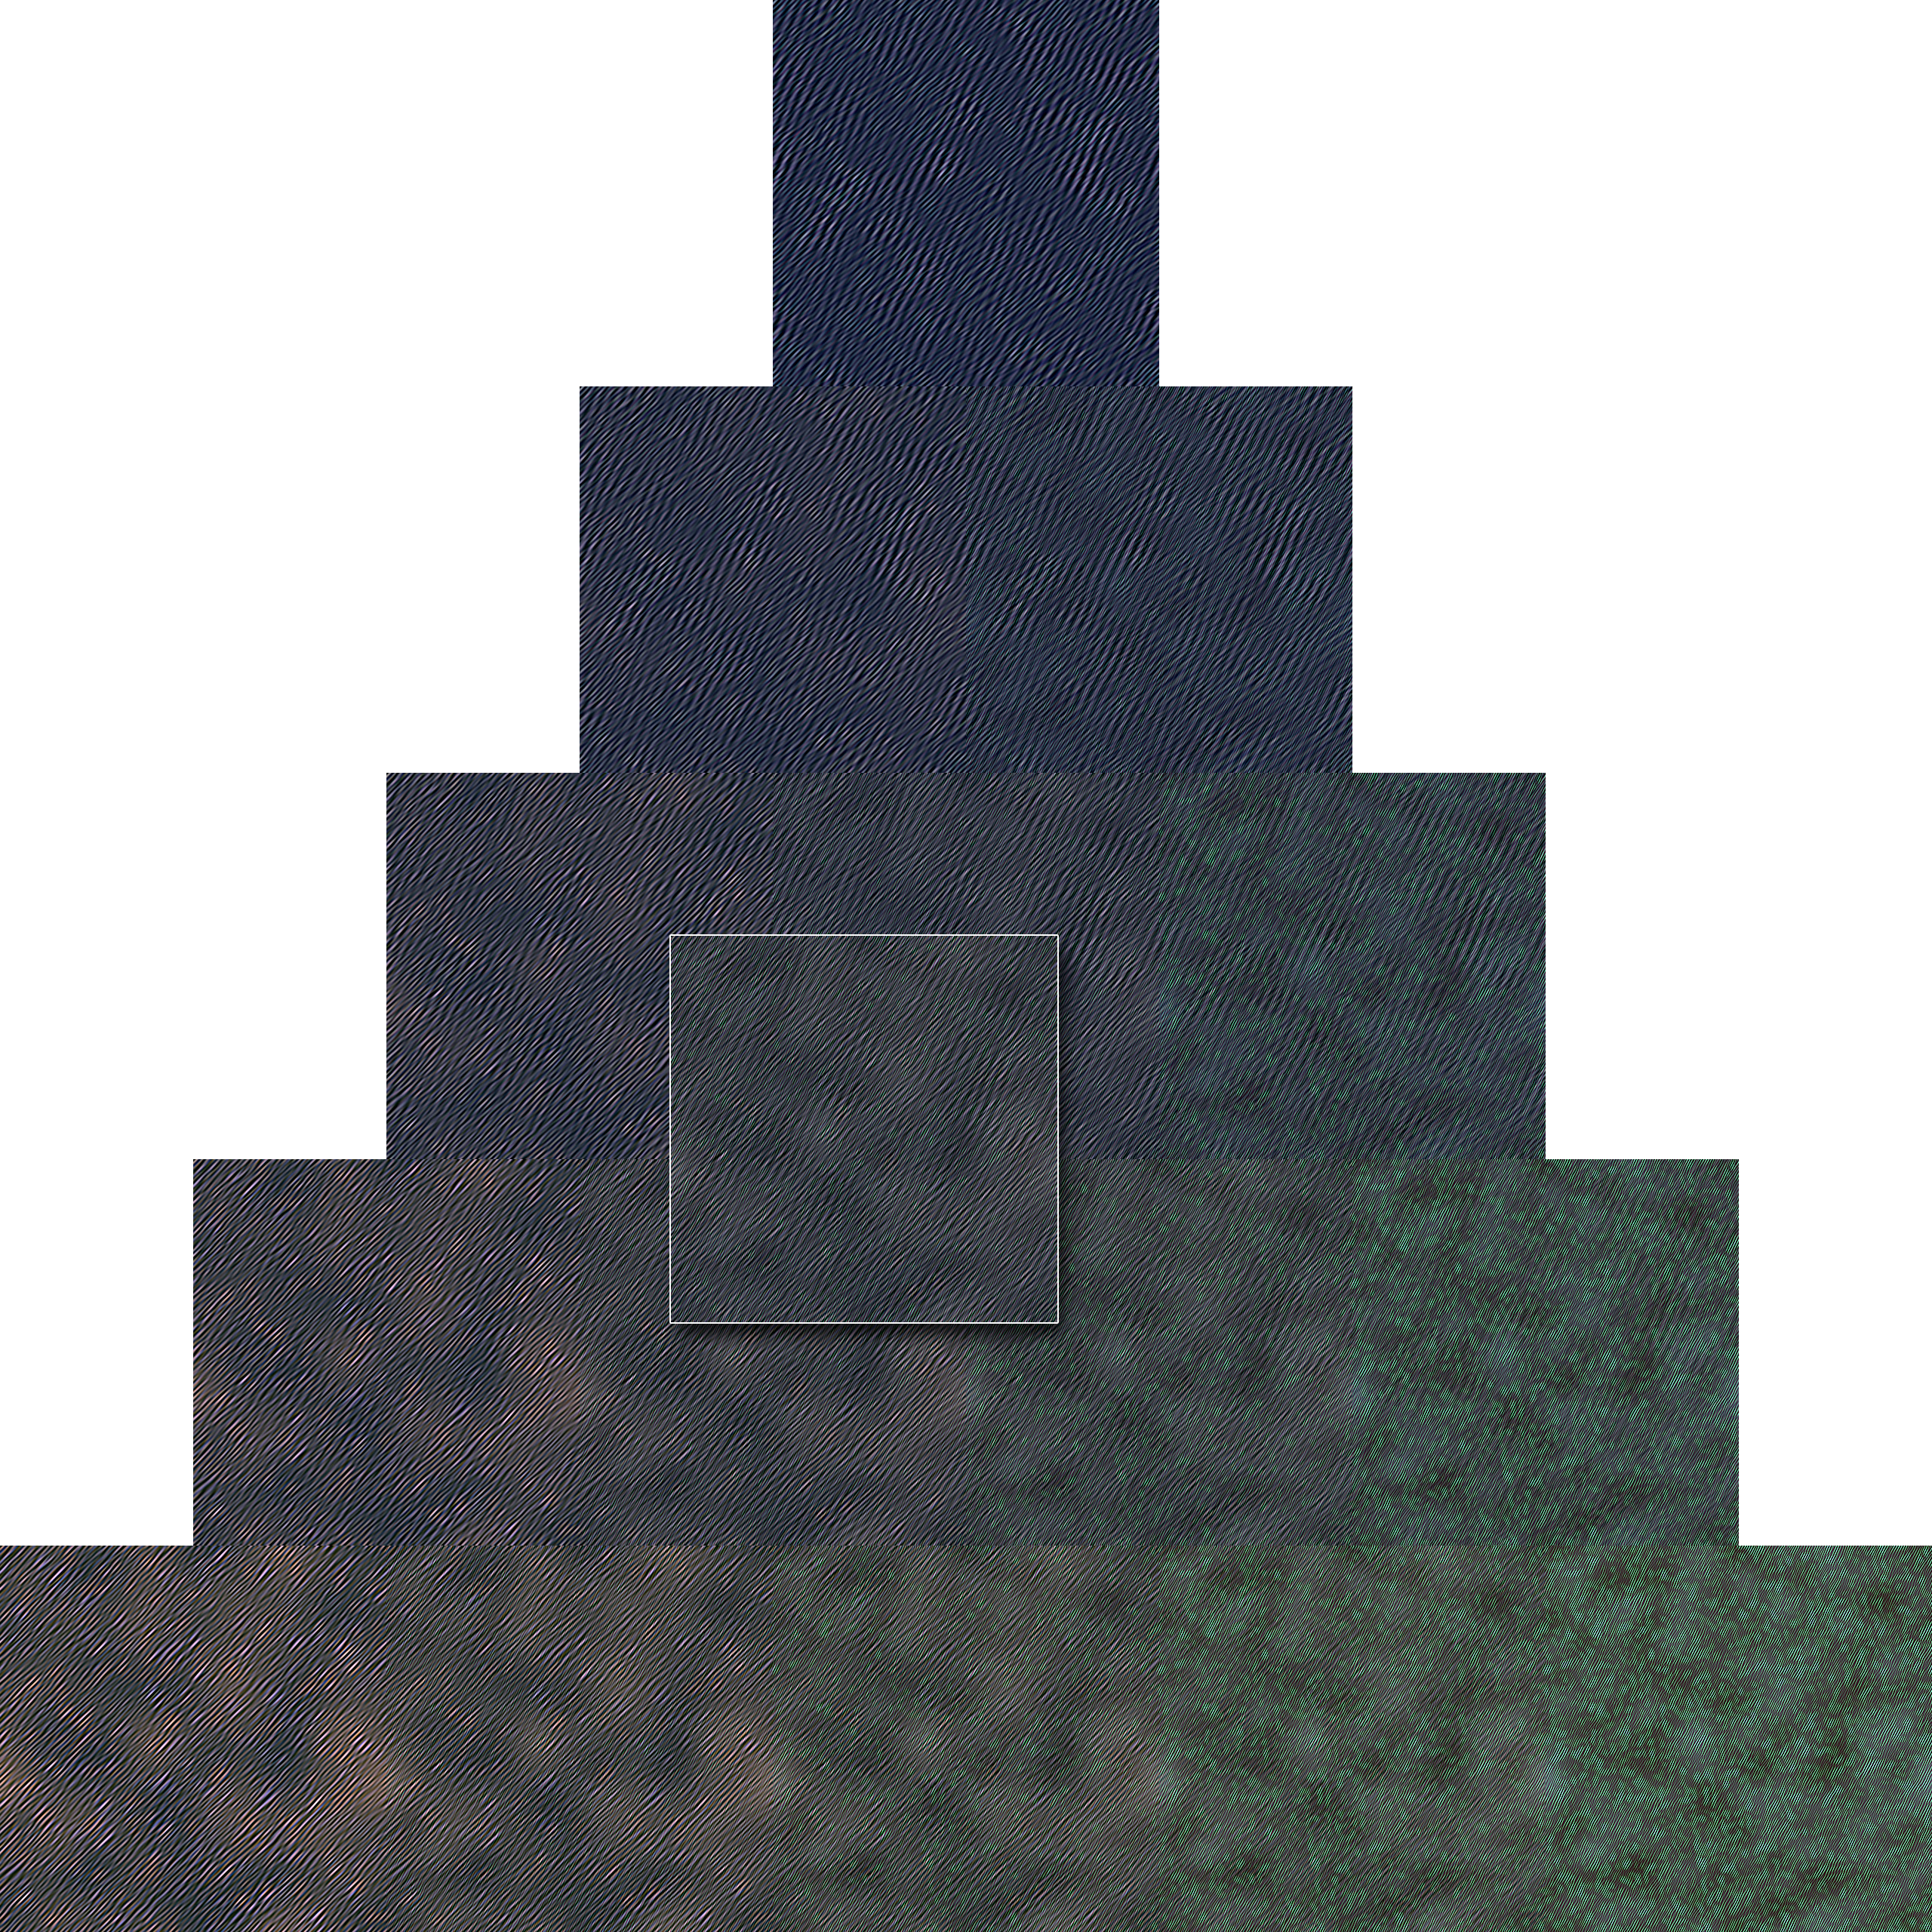
\includegraphics[width=0.49\linewidth]{textures/manC_Naive} \\
(a) Radon barycenter (our approach) & (b) Linear interpolation \protect{\cite{peyre2013Gaussians}}
\end{tabular}
\end{center}
\caption{(a) Eulerian Radon barycenter interpolates sparse amplitude spectra. (b) linear interpolation of the amplitude spectrum~\eqref{eq-interp-linear-spectrum}, as performed in \protect{\cite{peyre2013Gaussians}}. The top row shows the interpolated spectra $P_{F_\la}$.  }
\label{fig:texsynth}
\end{figure*}

\begin{figure*}[!t]
\setlength{\tabcolsep}{0pt}
  \setlength{\fboxsep}{0pt}
\begin{center} 
\begin{tabular}{ccc}
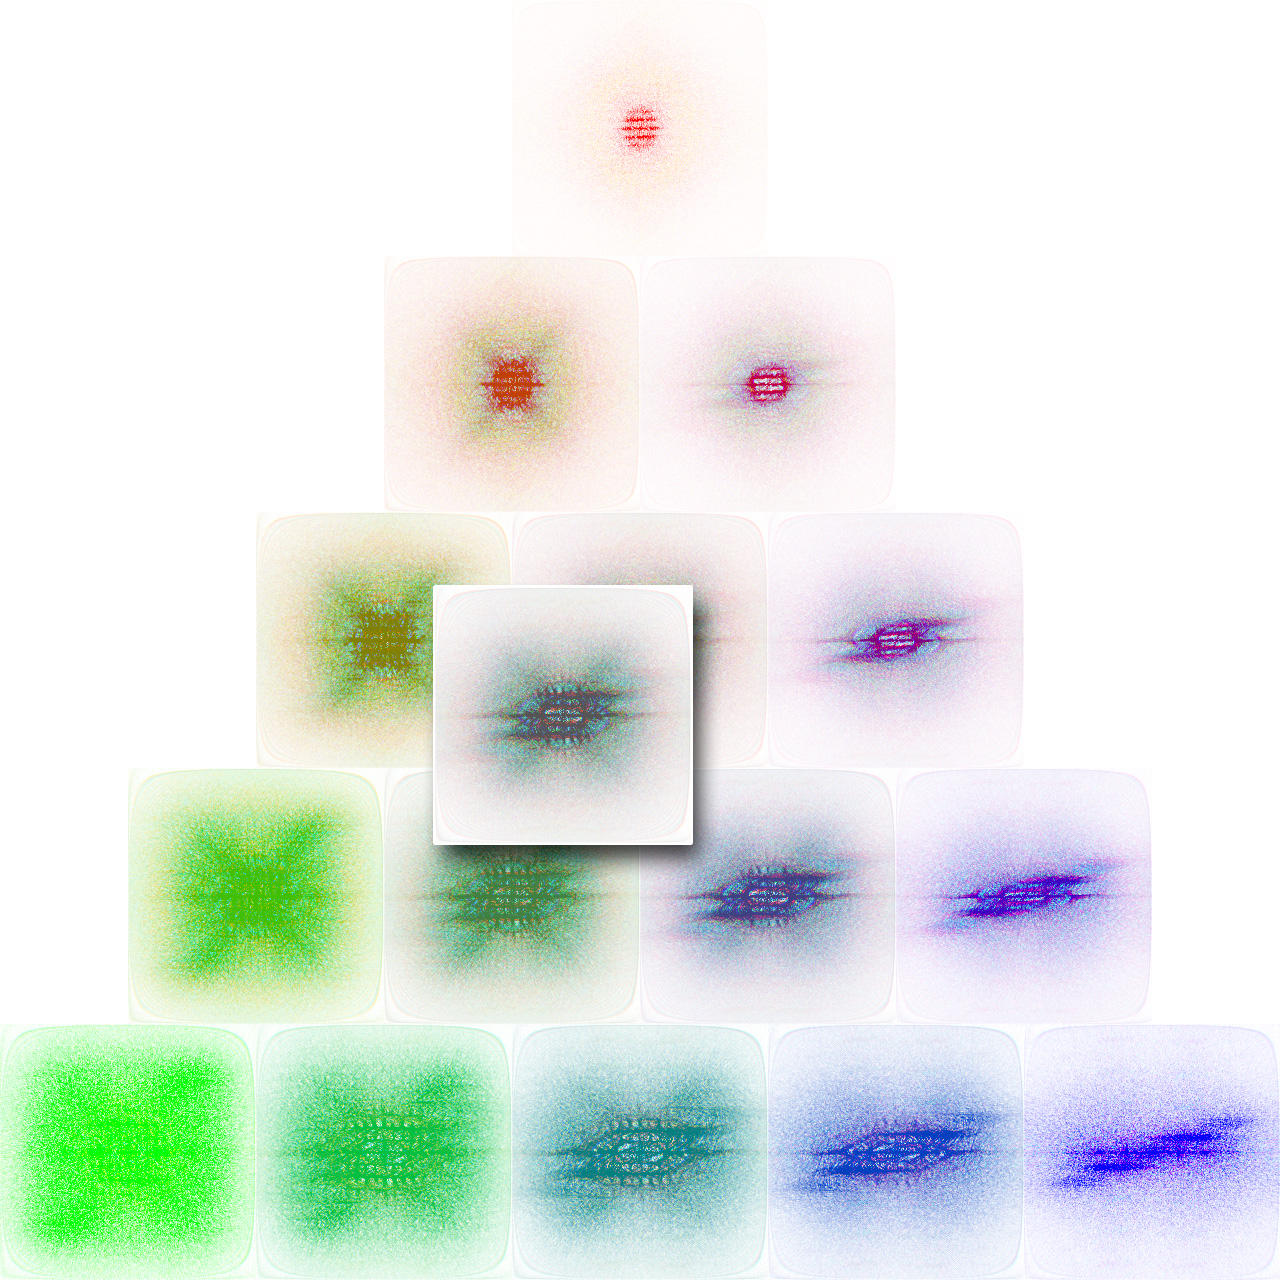
\includegraphics[width=0.48\linewidth]{textures/tex1spec_fastslant} &
 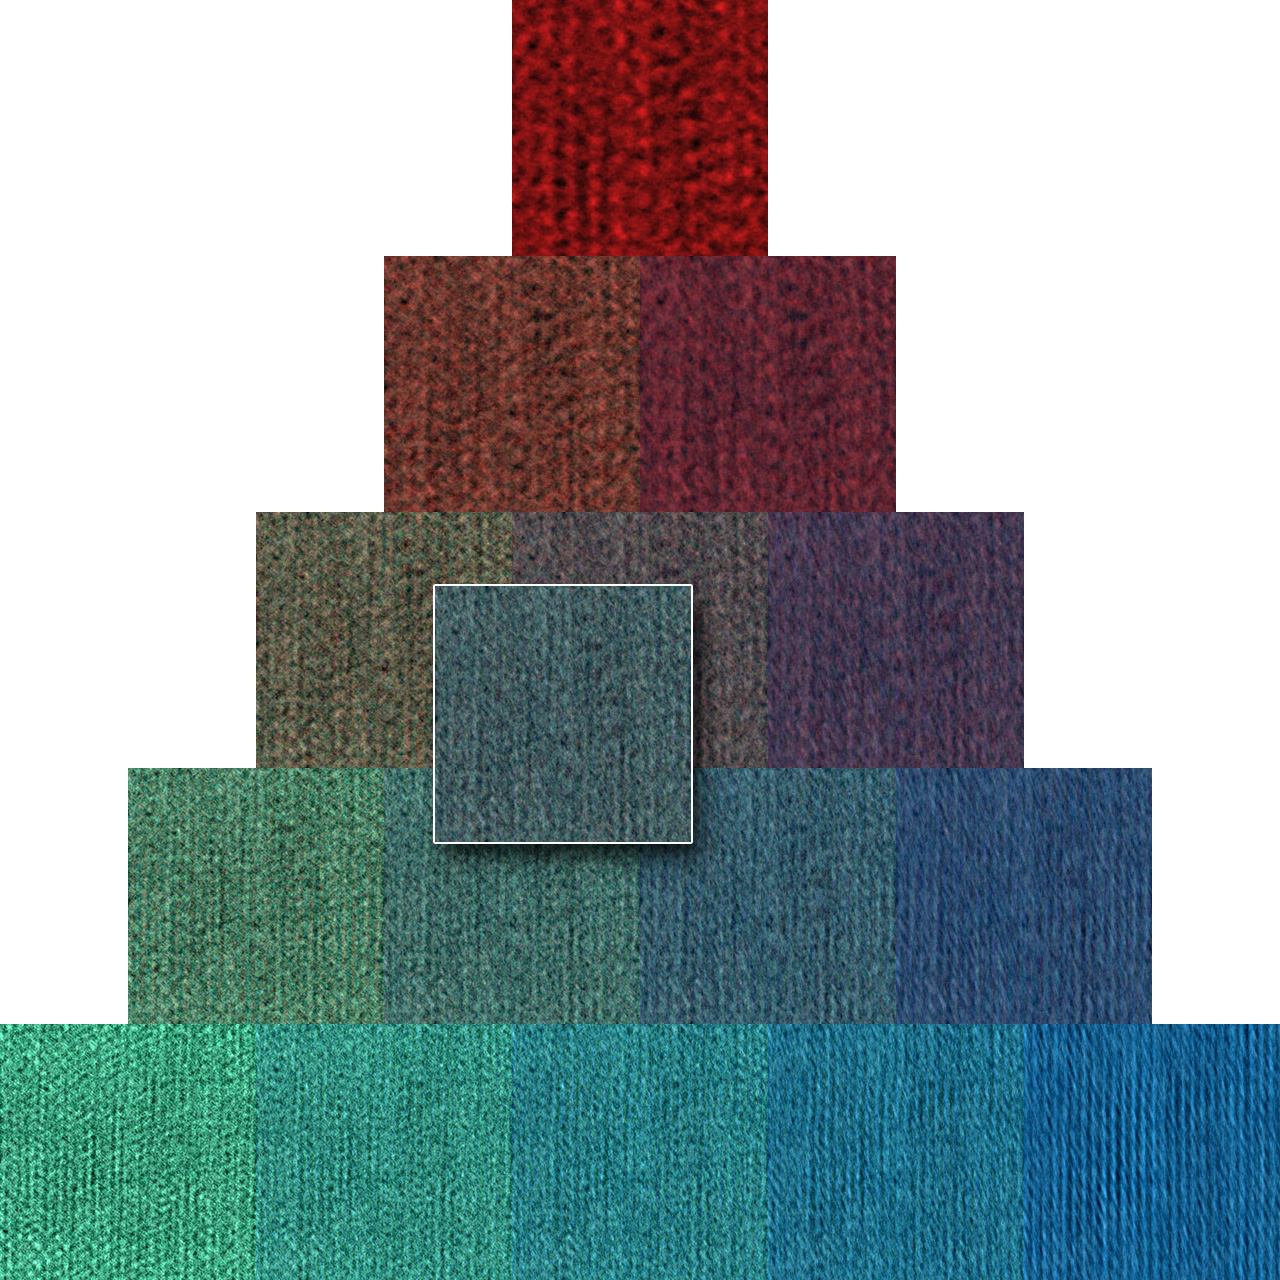
\includegraphics[width=0.48\linewidth]{textures/tex1fastslant} 
\end{tabular}
\end{center}
\caption{Eulerian Radon barycenter applied to the mixing of natural textures.}
\label{fig:texsynth2}
\end{figure*}

%%%%%
\paragraph{Comparison with linear interpolation.}

In~\cite{peyre2013Gaussians}, the authors also use optimal transport to perform SN model interpolation. Their approach is however radically different since they compute optimal transport geodesics in the space of Gaussian distributions in $\RR^N$, which has a closed form solution. In contrast, we propose to compute the transportation of PSD in $\RR^2$, viewed as discrete distributions of $N$ Diracs. For grayscale textures, the method detailed in~\cite{peyre2013Gaussians} thus boils down to a linear interpolation of the PSD, i.e., they define the PSD of the barycentric model $\tilde F_\la$ as
\eql{\label{eq-interp-linear-spectrum}
	\foralls \la \in \La_I, \quad
	P_{\tilde F_\la} = \sum_{i \in I} \la_i P_{F^{[i]}}.
} 
The effect achieved by our Radon barycenter differs from~\cite{peyre2013Gaussians}. As shown in Figure~\ref{fig:texsynth} and~\ref{fig:texsynth2}, we believe our method is geometrically more meaningful when dealing with textures that have a sparse Fourier expansion, while \cite{peyre2013Gaussians} deal with denser spectra more appropriately. Sparse spectra can occur, for instance, for textures with approximately periodic tiling of repetitive patterns. 



%%%%%%%%%%%%%%%%%%%%%%%%%%%%%%%%%%%%%%%%%%%%%%%%%%%
\subsection{Application to Color Palette Manipulation}
\label{sec-appli-colorization}

In this section we investigate the benefit of our Sliced Wasserstein barycenter for two applications: harmonizing colors in an image sequence, and grading colors of a single image. Color harmonization is the process of bringing the colors of input images to an average color distribution such that the images end up looking more similar. This has several applications such as, for instance, image stitching or enforcing temporal coherence of colors in movies. The second application allows for the editing of a single image by bringing its colors closer to a set of photographs exhibiting particular color palettes. This process is called color grading, and finds applications in photograph enhancement.


% In both cases, the method is a two step process. First, a color palette (i.e., color distribution) is computed using our barycenter. Then, the new color distribution is transferred to each input images using (approximate) optimal transport.

%\todo{I think it is simpler to avoid confusing the reader to make the method a two steps algorithm : first harmonization, then color transfer. } %Nico: I'm not sure what you mean here: is the above ok?

%%
\paragraph{Lagrangian color palette.}

We consider a color image represented as a vector $X \in \RR^{N \times 3}$ of $N$ pixels, so that $X = (X_k)_{k=1,\ldots,N}$ where each pixel $X_k \in \RR^3$ stores the value of a pixel indexed by $k$. 
In the following, we use the YCbCr color space because of its ability to decorrelate color channels, although other color spaces may be used (e.g., the CIE-Lab advocated in~\cite{Reinhard:2011}). 
The color distribution of this image is a measure $\mu_X$ defined in $\RR^3$, and describes the color palette.  We naturally represent this color distribution using a Lagrangian discretization, as defined in~\eqref{eq-lagrangian-discr}, by essentially storing pixel colors as a point cloud in the space of colors. Note that the Lagrangian discretization~\eqref{eq-lagrangian-discr} defining $\mu_X$ is automatically normalized so that $\mu_X \in \Mm_1^+(\RR^2)$. We hence compute the average distribution of multiple images distributions using our (Lagrangian) Sliced Wasserstein Barycenter detailed in Section~\ref{subsec-algorithm-lagrangian}.  

% The color point-cloud of the image $u$ is then obtained as $X_u = \left\{ (Tu)_k \right\}_{k\in M\times N} \in \R^{d\times MN}$, defining the color measure $\mu_u$ as a discrete sum of Dirac masses located in $(Tu)_k$, corresponding to the pixel $Tu(m,n)$ at location $k = m + (n-1)M$.

%%
\paragraph{Color palette transfer.}

Before detailing our main application to color palette barycenters, we illustrate our stochastic gradient descent (Section~\ref{subsec-sliced-assignement}). This descent allows for the computation of an approximate Sliced transport map $T^S$ between the color palette $\mu_{\iterInit{X}}$ of an input image $\iterInit{X}$ and the model palette $\mu_Y$ of an image $Y$, where $\iterInit{X},Y \in \RR^{N \times 3}$. The resulting image $X^\star$ is obtained as the limit of the stochastic gradient descent steps~\eqref{eq-stoch-grad-desc} until convergence
\eql{\label{eq-converg-colorization}
	\iter{X} \overset{\iterInd \rightarrow +\infty}{\longrightarrow} X^\star, 
}
as described in~\eqref{eq-lim-xstar}. 

%\paragraph{Comparison with~\cite{pitie2005n}}
We illustrate our technique in Fig.~\ref{fig:colortransfer2}. This process generalizes the algorithm introduced in~\cite{pitie2005n} that uses $|\Th_\iterInd|=3$ orthogonal directions at each step. 
%Figure~\ref{fig:colortransfer2} shows a comparison of the result obtained with $|\Th_\iterInd|=10$ orientations and the method of~\cite{pitie2005n}. To illustrate differences in the choice of orientations, we did not use any regularization, used the same RGB color space, and kept the number of iterations fixed to 20. This shows that using more directions reduces the visual artifacts created by the transport. 
While we make use of an exact Lagrangian method by sorting pixel values, Piti\'{e} et al. discretize histograms and use the cumulative histogram and pseudo-inverse approach (Eqs.~\ref{eq-cumulative-defn} and \ref{eq-cumulative-pseudoinv-defn}). The lower complexity of ~\cite{pitie2005n} comes at the expense of a discretization which can lead to quantization errors and limits convergence. 


% \cmt{
% The main differences of this approach in comparison to ours are:
% \begin{itemize}
% \item it makes use of cumulative histograms \eqref{eq-cumulative-defn} and pseudo-inverse \eqref{eq-cumulative-pseudoinv-defn} to perform 1-D histogram matching iteratively. In practice, this requires a quantization process for computing both histograms and inverse cumulative function, leading to color approximations and quantization error, so that the algorithm does not properly converge. The resulting color histogram is still very close to the target one in practice. % Nico: si on dit que ca ne converge pas de maniere forte, il faut montrer des plots, des tests, etc. On peut faire ca, mais on peut aussi nous dire que "peu importe puisque ca donne de jolis resultats quand meme"... Le but n'est pas non plus de basher Pitie qui va peut etre nous reviewer ;)

% \item the time complexity of this approach is linear $O(q)$ in the number of quantized colors $q$ (observe that the quantization must be performed simultaneously for both input and target color palettes, but also for color quantiles), whereas ours makes use of a sorting algorithm and results therefore in $O\big(N\log(N)\big)$. % Nico: donc notre approche est plus complexe (sauf a utiliser plus de bins que de pixels...!). On va pas insister dessus hein ;)

% \item the basis direction set $\Theta^{[k]}$ to be used at iteration $k$ is precomputed in order to minimize the correlation with previous directions;  % Nico: Je ne pense pas que ca soit important (sinon faut dire pourquoi ca l'est). On pourrait faire pareil par exemple, et on pourrait nous demander pourquoi on fait pas ca.

% \end{itemize}
% }

%\todo{what is smoother? pitie? ours? the wasserstein plan that we both approximate?}.  \todo{Apparently, using more direction leads to a better transport ? Is it correct ? Why ? Some more comments are needed.} \todo{Also note that I directly too Pitie's code ; the regularization might be different etc. I was more intending a qualitative comparison}
%\cmt{Julien : Piti� ne fournit pas le code pour la r�gularisation, mais seulement pour le transfert de couleur, ce qui donne des artefacts.}



% Note that transferring the colors of an image to another can be performed with our stochastic gradient descent, which directly generalizes the method proposed in~\cite{pitie2005n}. The algorithm proposed by Piti\'{e} et al.~\cite{pitie2005n} corresponds to our stochastic gradient descent when the subset of orientations $\Th_\iterInd$ chosen at each iteration is a set of three orthogonal directions drawn uniformly at random. We do not impose this restriction. A color transfer result can be see in Fig.~\ref{fig:colortransfer2}.

\begin{figure}[!t]
%
\begin{center} 
\begin{tabular}{@{}c@{\hspace{2mm}}c@{}}
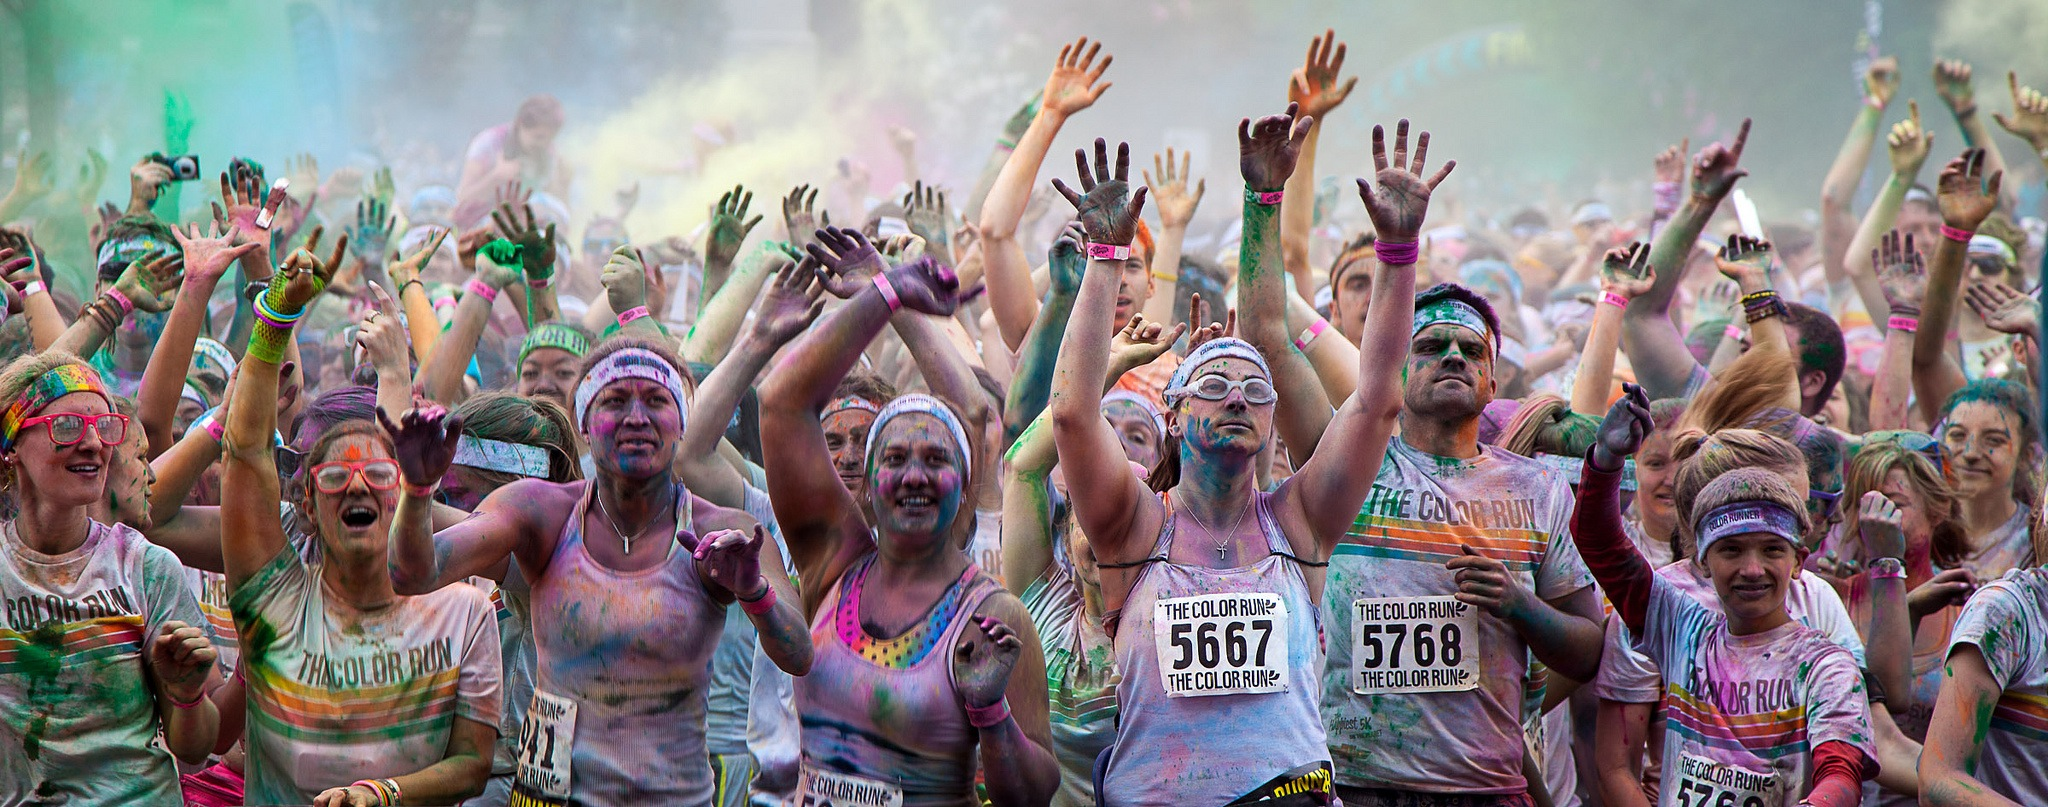
\includegraphics[height=2cm]{color/8733654151_b9422bb2ec_k} &
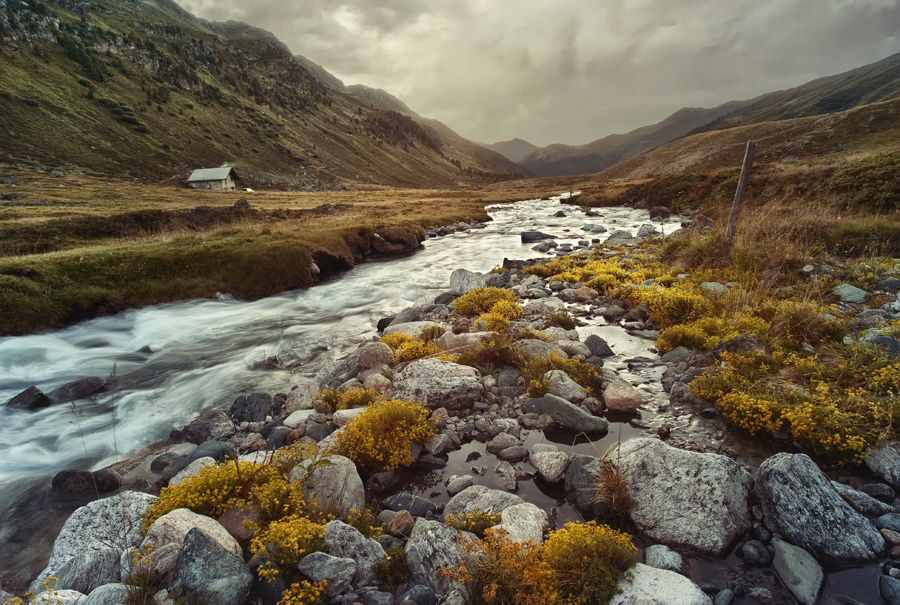
\includegraphics[height=2cm]{color/4852775794_c671f133d0_b} \\
(a) input image $\iterInit{X}$  & (b) input model $Y$ \\
\end{tabular}
\begin{tabular}{@{}c@{}}
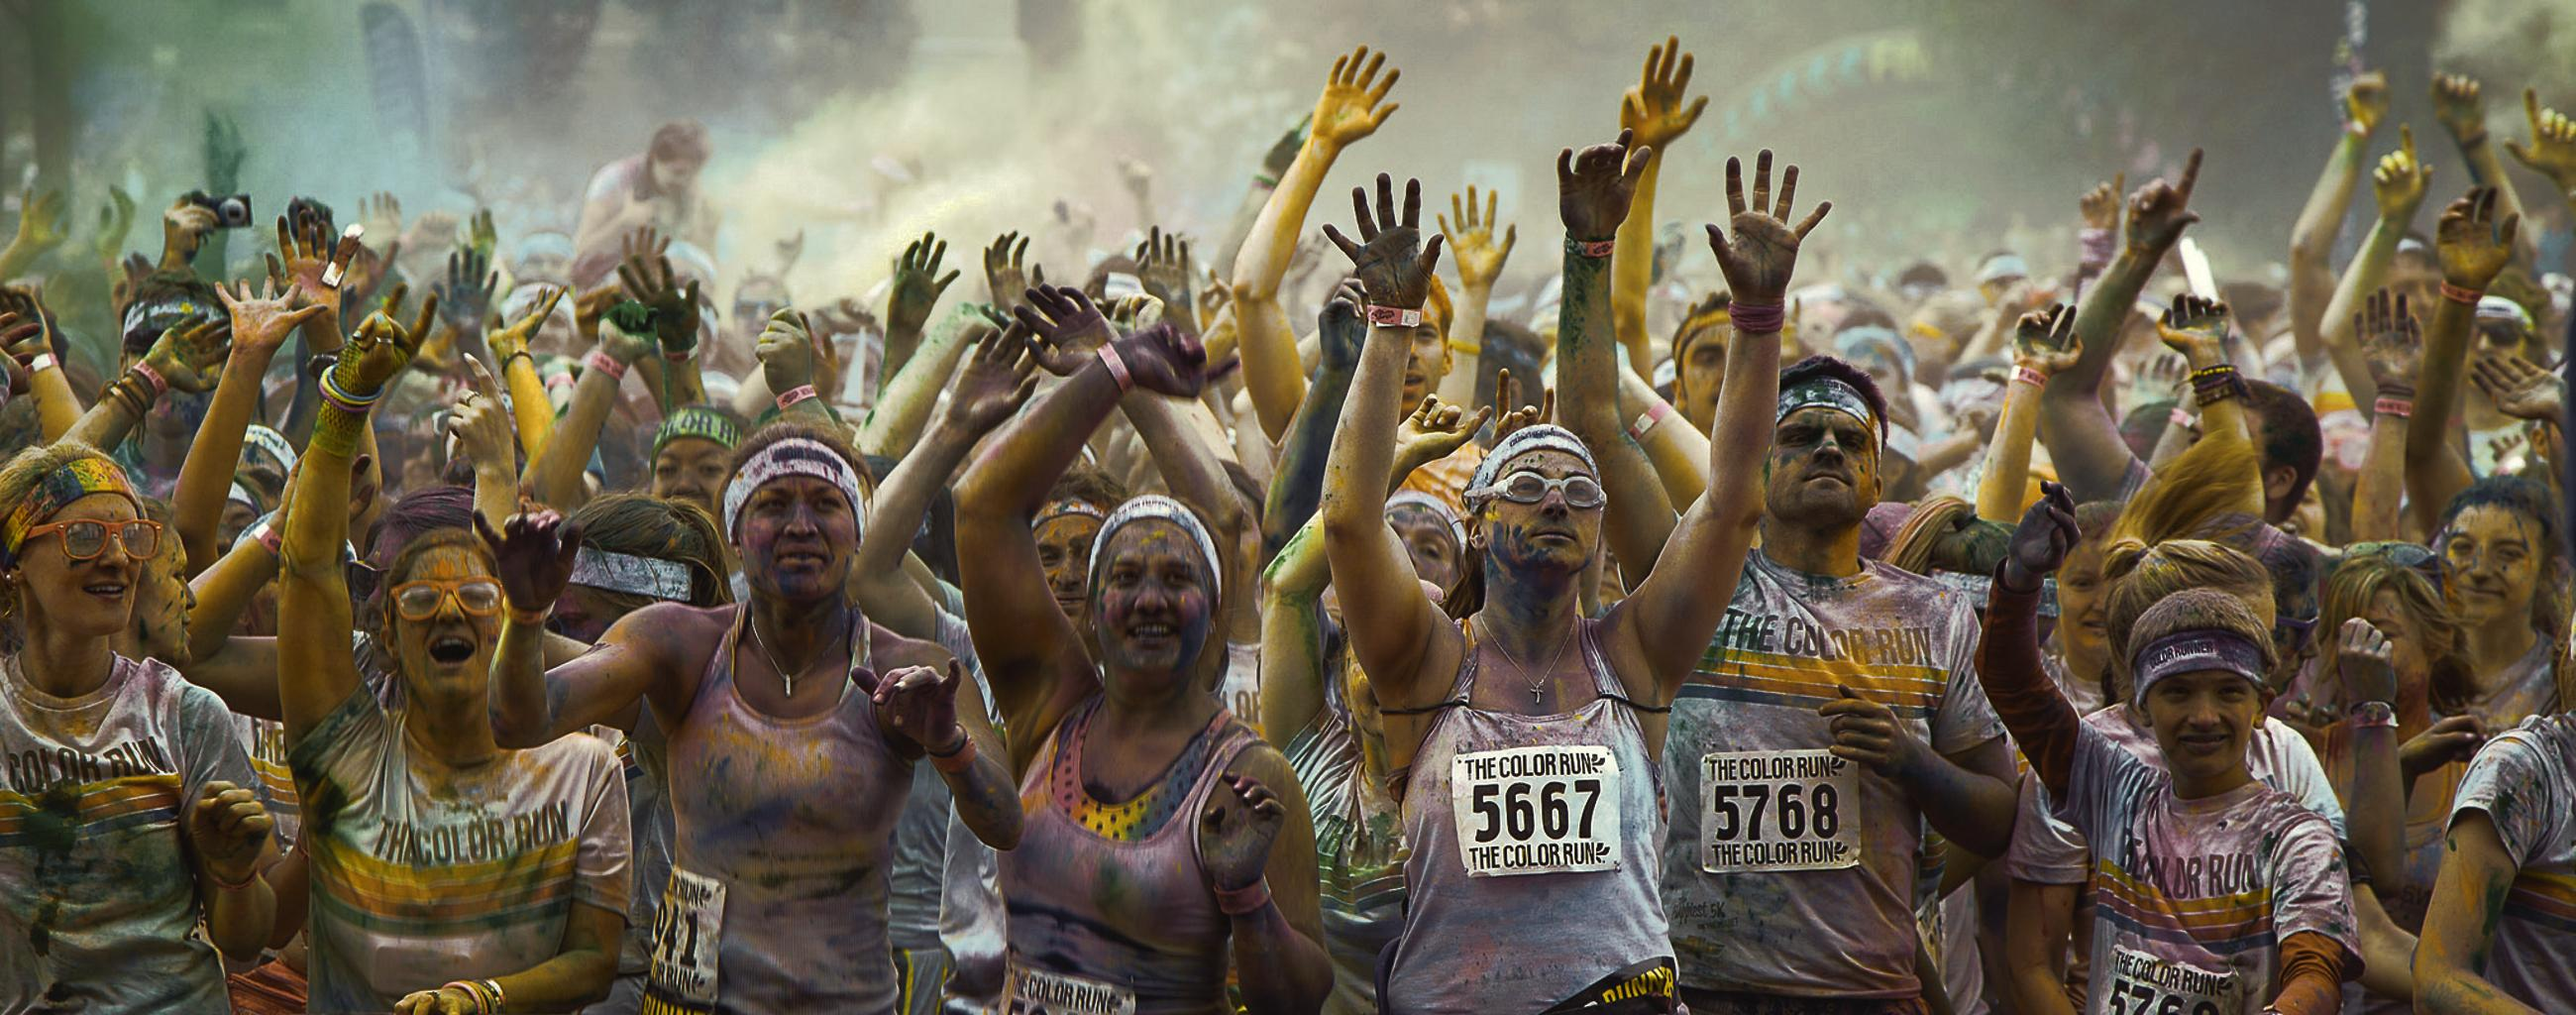
\includegraphics[width=\columnwidth]{color/color_transfer_20iters_noreg_rgb_10dirs}\\ 
(c) our result $X^\star$ 
\end{tabular}
\vspace{-0.2cm}
\end{center} 
%
\caption{Our stochastic gradient descent (c) can be used to transfer the colors of a model image (b) to an input image (a). We generalize the method of Piti\'{e} et al.~\protect{\cite{pitie2005n}} as described in Sec.~\ref{sec-appli-colorization}
%\cmt{Julien : pour �tre ``fair'', il faut que l'on enl�ve la r�gularisation} %ok
}
\label{fig:colortransfer2}
\end{figure}


%%
\paragraph{Color palette barycenter.}

% Let $\{u^{(i)}\}_{i\in I}$ be the color-sequence and 

We consider a set $\{X^{(i)}\}_{i\in I}$ of color images, as well as a particular input color image $\iterInit{X}$. Using~\eqref{eq-non-convx-pointclouds}, we define the color palette $\mu_{X^\star}$, the barycenter of the input palettes $\mu_{X^{(i)}}$, as the Sliced Wasserstein barycenter\\ 
%\eq{
	$\mu_{X^\star} \approx \Bary{\RR^d}^S\pa{ 
			\mu_{X^{(i)}}, \la_i 
		}_{i\in I}$
%}
with weights $\lambda \in \La_I$. 

%%%
\paragraph{Color image harmonization and color grading.}

In order to adjust colors in an image, we are interested in an image $X^\star$ visually similar to $\iterInit{X}$, but whose palette closely matches the palette barycentre $\mu_{X^\star}$. Similarly to the simple color transfer application (see~\eqref{eq-converg-colorization}), we obtain this image by performing the gradient descent iterations~\eqref{eq-grad-desc-sliced} with initialization $\iterInit{X}$, and define $X^\star$ as the limit image $	\iter{X} \overset{\iterInd \rightarrow +\infty}{\longrightarrow} X^\star$.

However, highly non-linear color transformations can create undesirable visual artifacts. We therefore use an iterative post-processing technique introduced in~\cite{Rabin_artefact} to regularize the transportation map $\iterInit{X}_k \mapsto X^\star_k$. We refer the interested reader to~\cite{Rabin_artefact} for further details. 
% We still denote as $X^\star$ the final harmonized imaged obtained after this pre-processing. 

%We use our technique for manipulating colors. 
For color harmonization,  we apply this process successively to each image in an input sequence $\{ X^{(i)} \}_{i \in I}$, by initializing $\iterInit{X}$ with $X^{(i)}$ for each $i$. %We denote our resulting images $X^{(i,\star)} \leftarrow X^\star$.  \cmt{Nico: why would we introduce a notation that we won't use?}
For color grading, we instead apply the palette barycenter to an arbitrary input image $\iterInit{X}$. %, which is, in general, different from any of the input images in $\{ X^{(i)} \}_{i \in I}$. 

\begin{figure*}[!t]
\begin{center} 
\raisebox{-0.5\height}{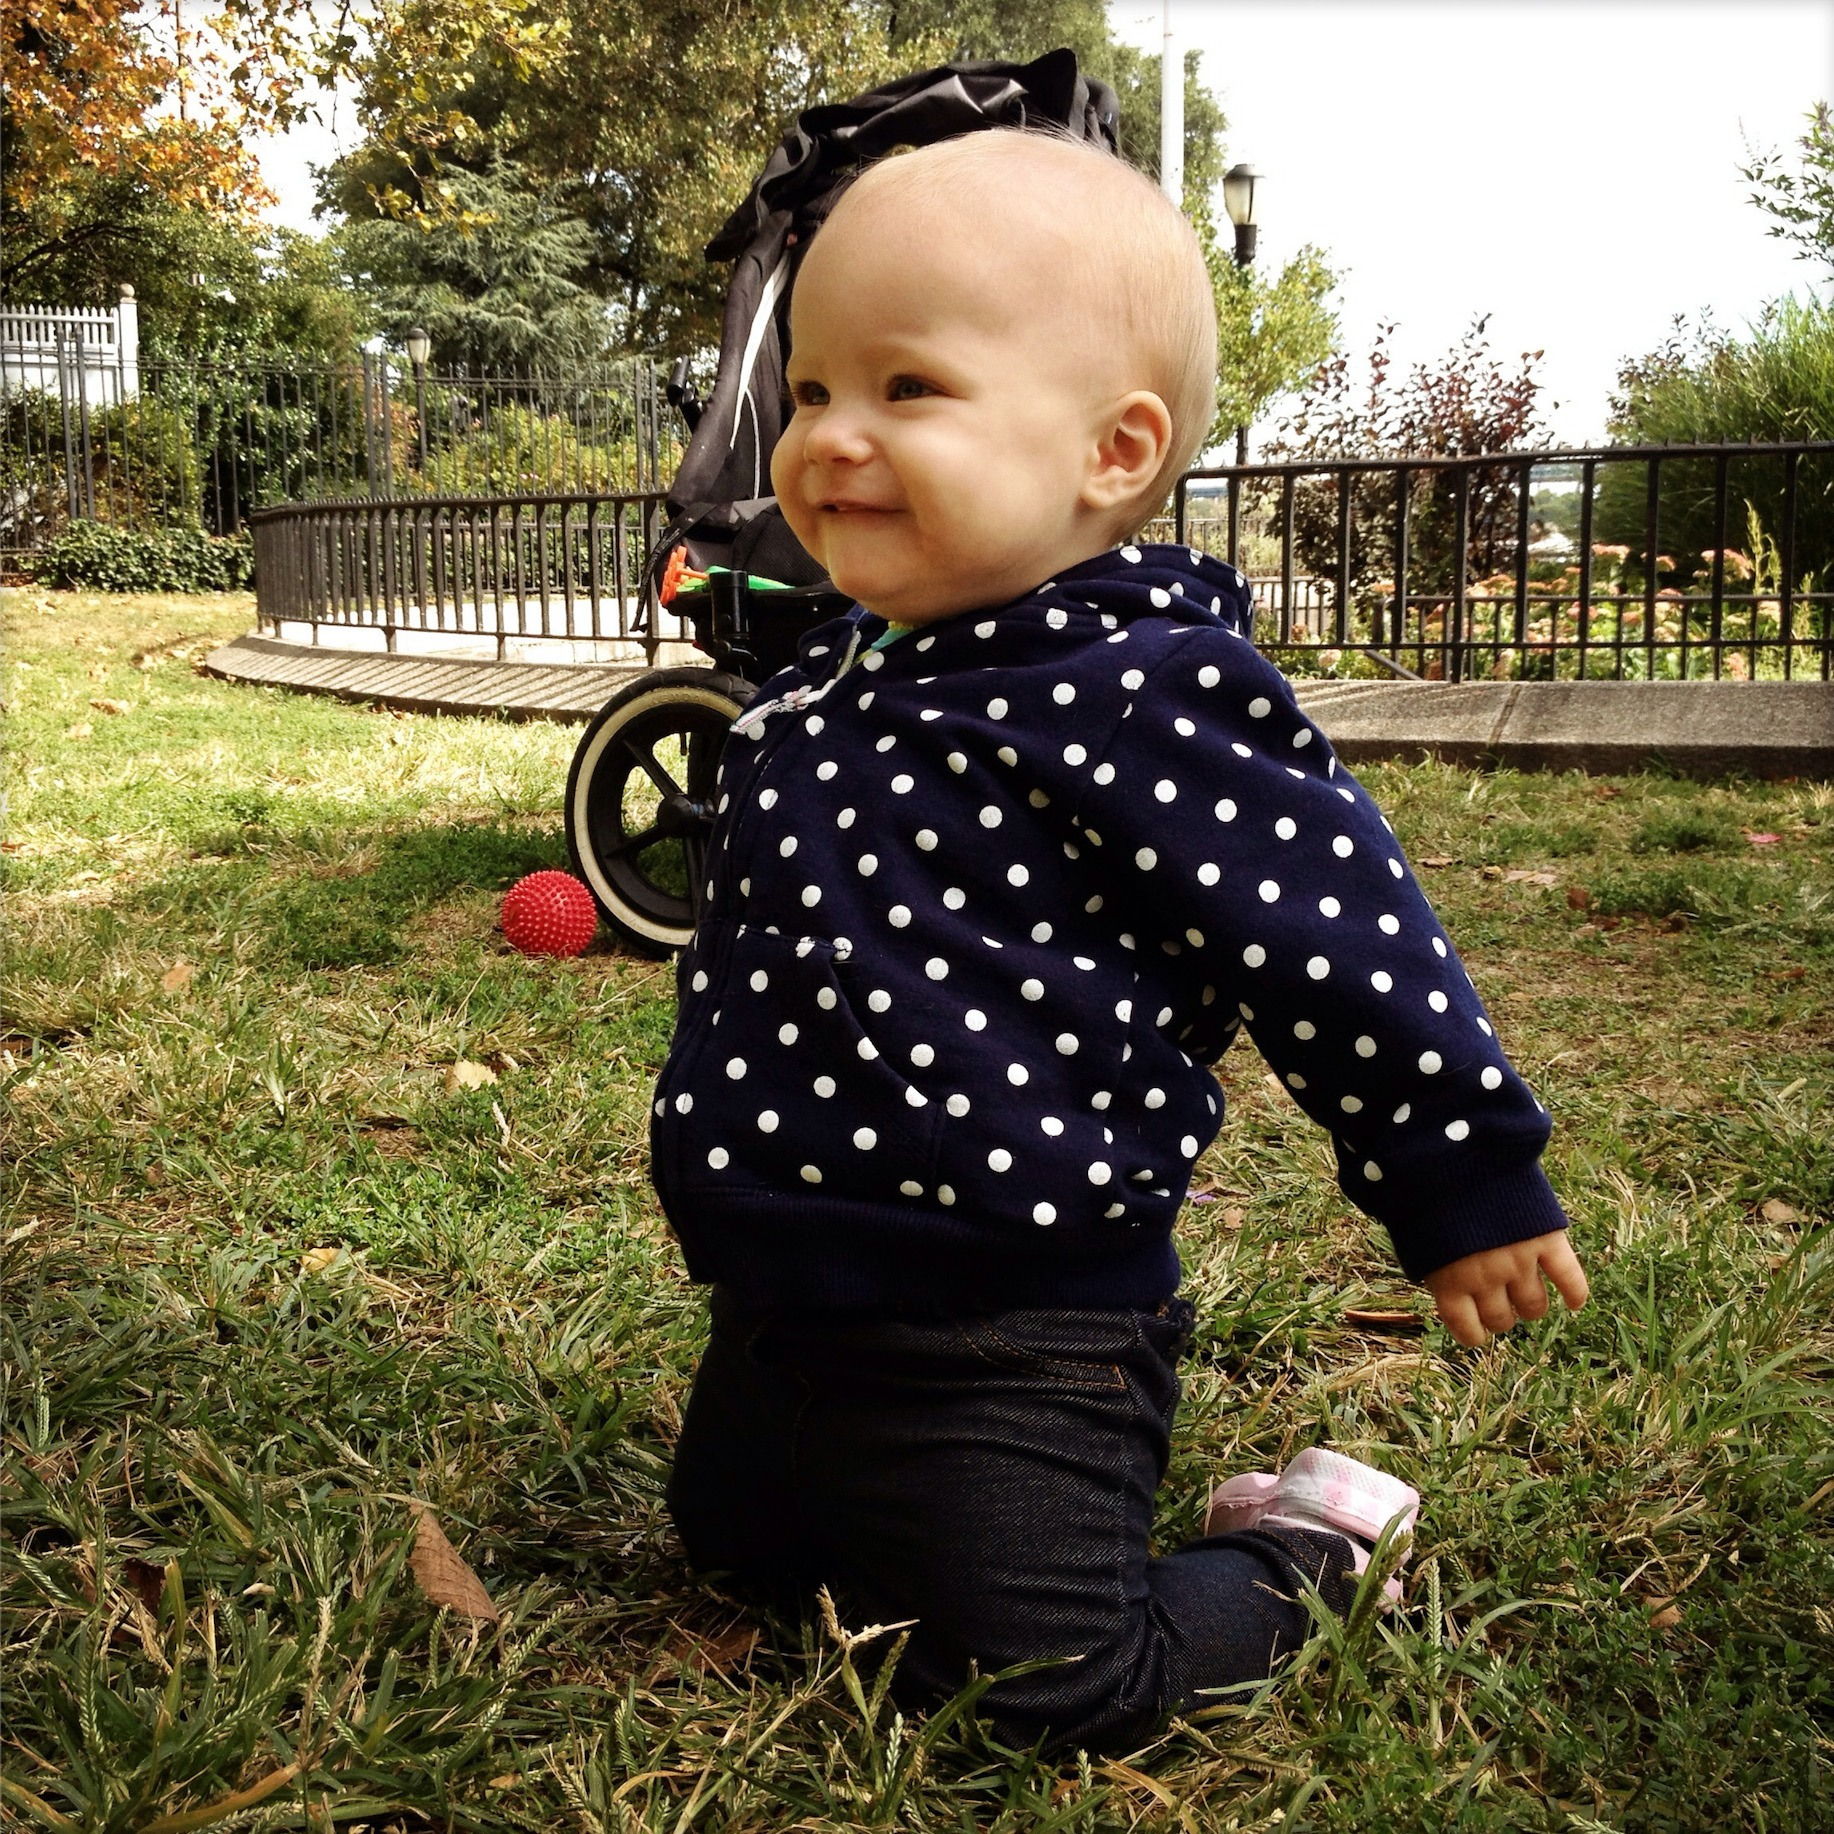
\includegraphics[width=0.2\linewidth]{color-samples/9768152396_c7be0b47bd_o}}
\raisebox{-0.5\height}{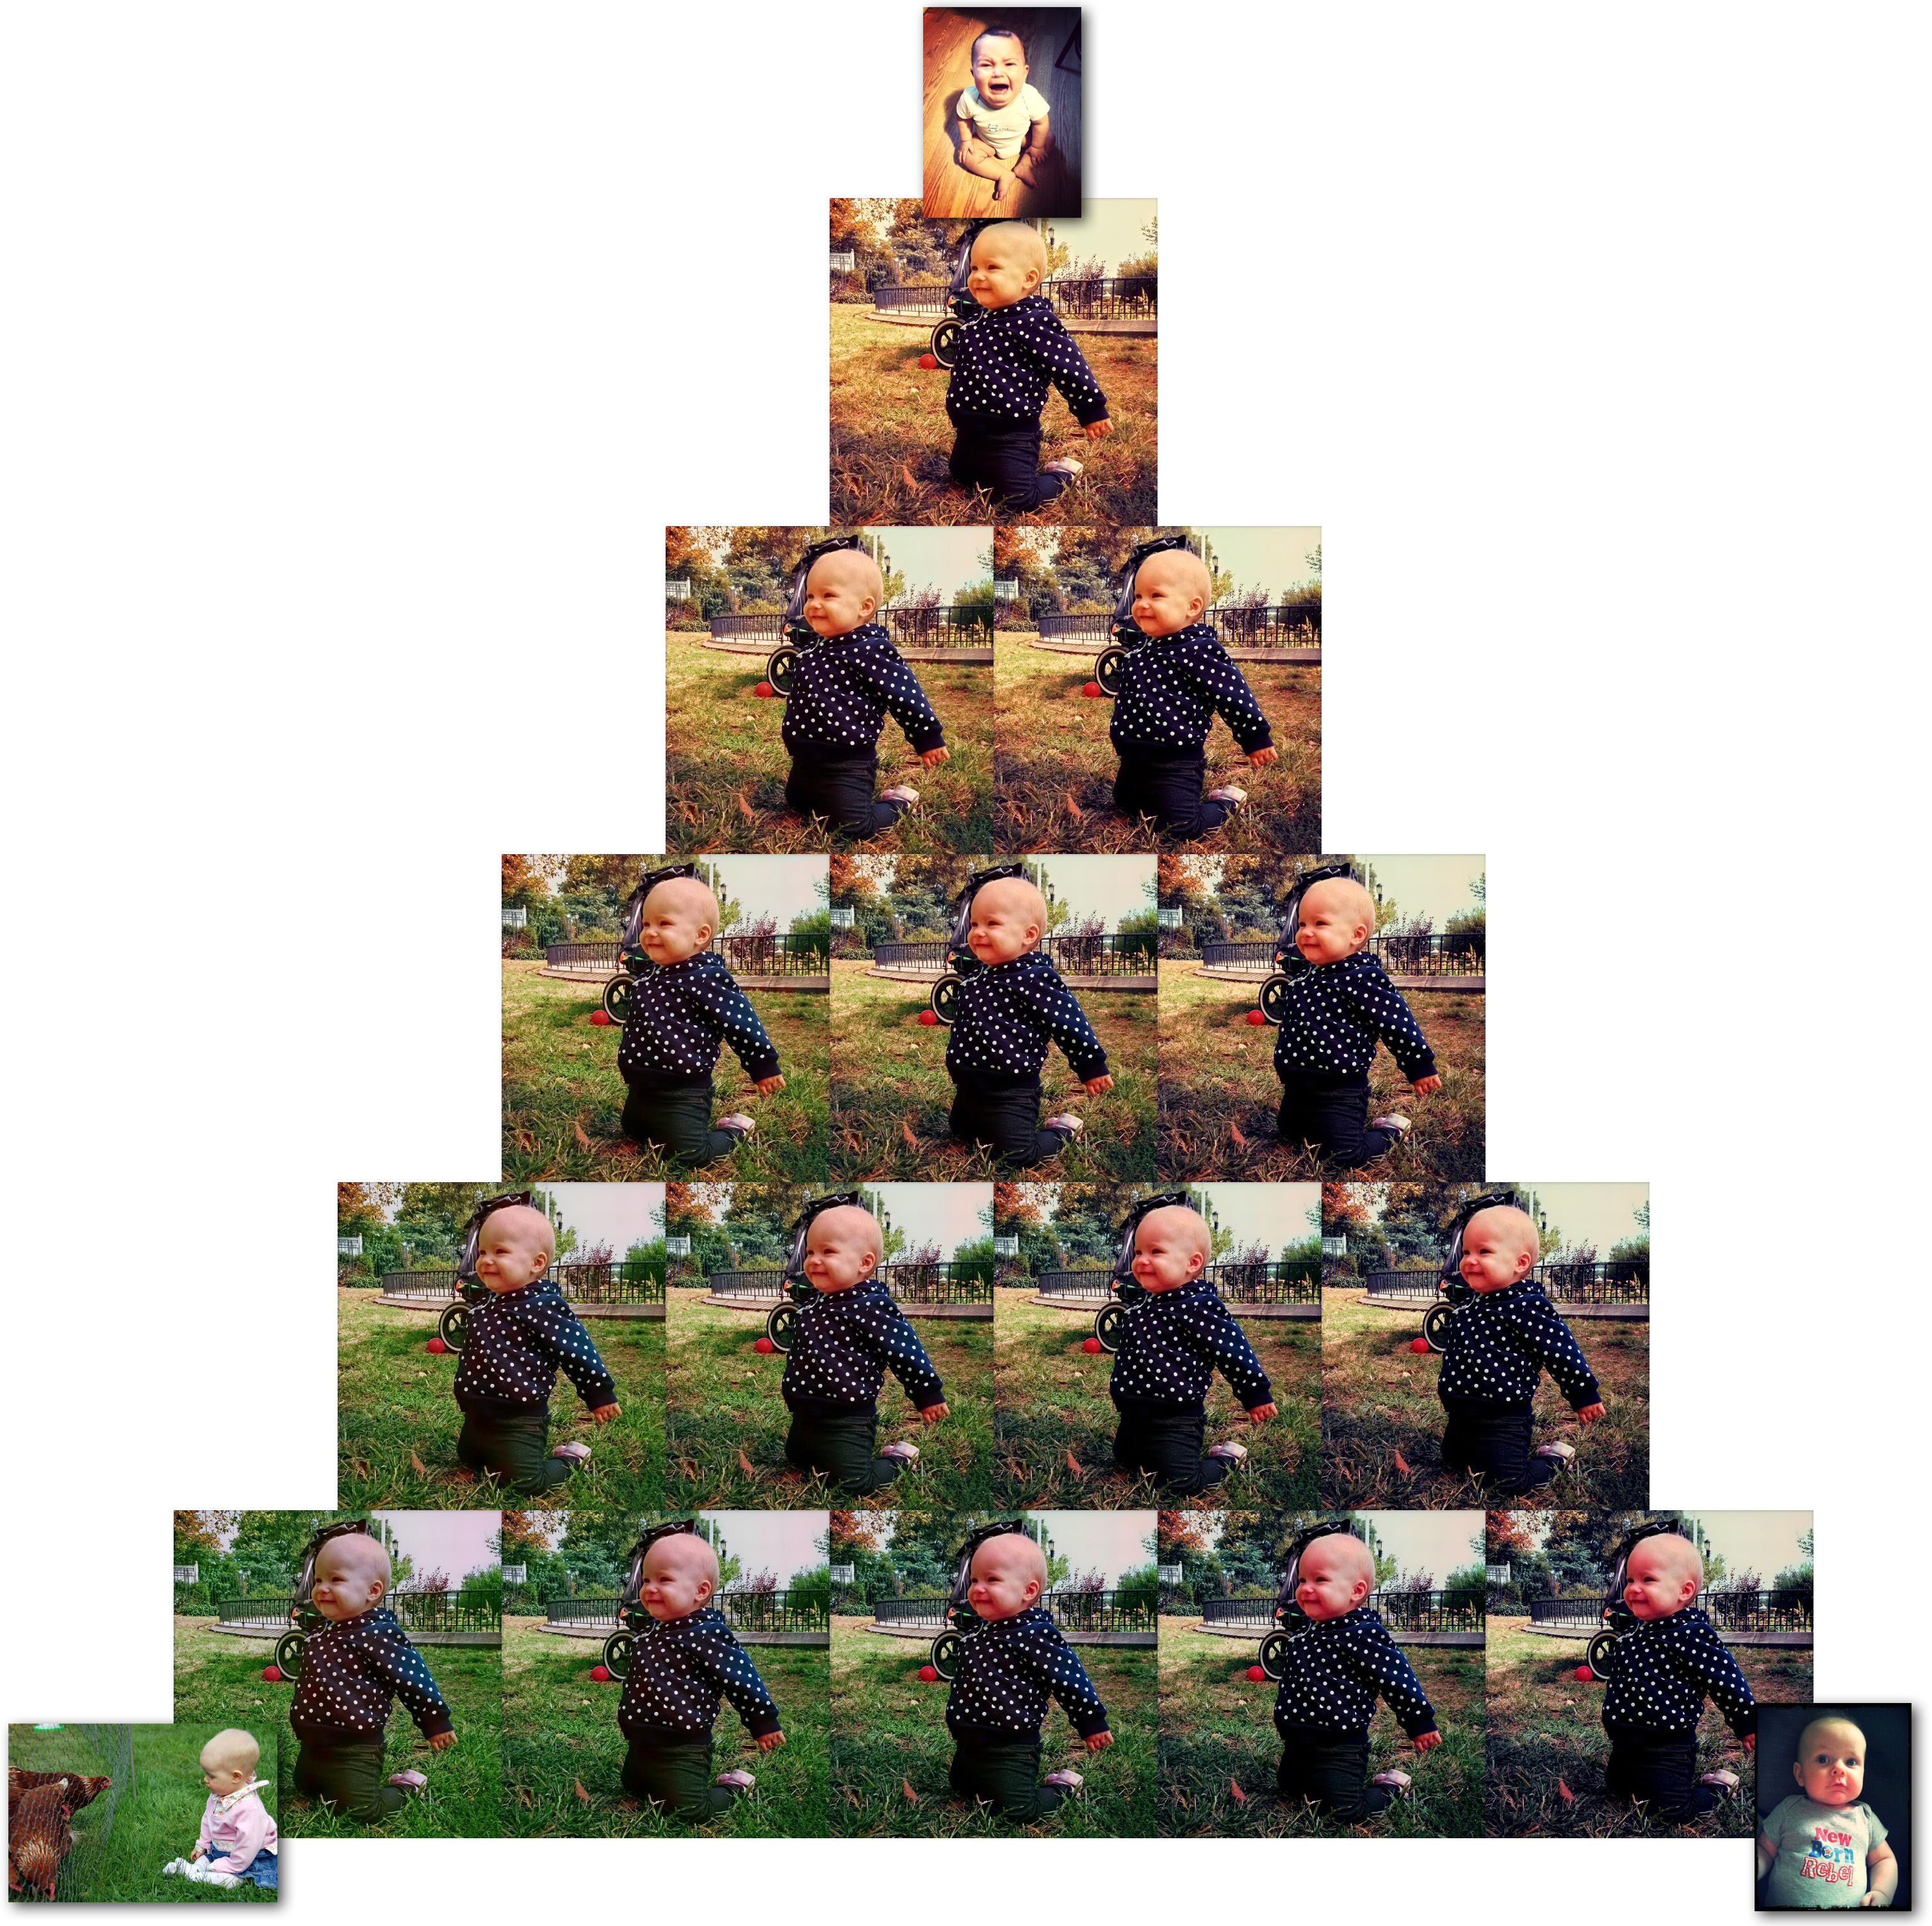
\includegraphics[width=0.65\linewidth]{color2/Proj_H_ok}}\\
\raisebox{-0.5\height}{\includegraphics[width=0.2\linewidth]{color-samples/3629553810_f27623de46_o}}
\raisebox{-0.5\height}{\includegraphics[width=0.65\linewidth]{color2/ProjF_ok}}
\end{center}
\caption{Color manipulation by transferring the colors of $|I|=3$ photographs $\{X_i\}_{i \in I}$ (shown at the vertices of the triangle, right) to the initial photograph $\iterInit{X}$ (left) to obtain $X^\star$ which varies in the triangle as a function of the convex weights $\la \in \La_I$. Additional results can be seen in supplemental material.}
\label{fig:colortransfer}
\end{figure*}

%%
\paragraph{Examples.}


\begin{figure}[!t]
\begin{center} 
\includegraphics[width=0.3\linewidth]{color/clockmontague-1} \hspace{1mm}
\includegraphics[width=0.3\linewidth]{color/clockmontague-2}  \hspace{1mm}
\includegraphics[width=0.3\linewidth]{color/clockmontague-3} 
\\
Original images $(X^{(i)})_{i \in I}$.\\ 
\includegraphics[width=0.3\linewidth]{color/Bary_Reg_clockmontague-1} \hspace{1mm}
\includegraphics[width=0.3\linewidth]{color/Bary_Reg_clockmontague-2}  \hspace{1mm}
\includegraphics[width=0.3\linewidth]{color/Bary_Reg_clockmontague-3} 
\\
Harmonized images $\{ X^{(i,\star)} \}_{i \in I}$. 
\end{center}
\vspace{-0.2cm}
\caption{Color harmonization of an image sequence, using $\la_i=1/|I|$ to compute the iso-barycenter (here $|I|=3$). }
\label{fig:colorharmonization}
\end{figure}


Figure~\ref{fig:colorharmonization} shows an example of harmonization, where the color palette is defined as the iso-barycenter of three input color palettes. In Figure~\ref{fig:colortransfer}, the image $\iterInit{X}$ to be modified is not contained in the set of input pictures $\{X^{(i)}\}_{i\in I}$. This allows for the user to navigate over the simplex of color palettes to select the desired one. Table~\ref{tab:weights} provides the corresponding weights for Figure~\ref{fig:colortransfer}.
% Nico: a simplex is necessarily convex, right?


\begin{table}
\caption{Coordinates $w$ used to define the weights $\lambda = w/(\sum_i w_i)$  for the color transfer in Figure~\ref{fig:colortransfer}.}
\label{tab:weights}
\begin{center}
\begin{tabular}{cccccccccc} % |c|c|c|c|c|c|c|c|c|c|
   %\hline
  \multicolumn{4}{c}{  } & \multicolumn{2}{c}{ $\sf (0,0,1)$ } \\
   %\hline
   \multicolumn{3}{c}{  } & \multicolumn{2}{c}{ $\sf (1,0,3)$ } & \multicolumn{2}{c}{ $\sf (0,1,3)$ } \\
   %\hline
   \multicolumn{2}{c}{  } & \multicolumn{2}{c}{ $\sf (1,0,1)$ } & \multicolumn{2}{c}{ $\sf (1,1,2)$ } & \multicolumn{2}{c}{ $\sf (0,1,1)$ } \\
   %\hline
   {\color{white} $\sf (0,$} & \multicolumn{2}{c}{ $\sf (3,0,1)$ } & \multicolumn{2}{c}{ $\sf (2,1,1)$ } & \multicolumn{2}{c}{ $\sf (1,2,1)$ } & \multicolumn{2}{c}{ $\sf (0,3,1) $}  \\
   %\hline
   \multicolumn{2}{c}{ $\sf (1,0,0)$ }  & \multicolumn{2}{c}{ $\sf (3,1,0)$ } & \multicolumn{2}{c}{ $\sf (1,1,0)$ } & \multicolumn{2}{c}{ $\sf (1,3,0)$ } & \multicolumn{2}{c}{ $\sf (0,1,0)$ }  
   %\hline
\end{tabular}
\end{center}
\end{table}


% \begin{figure*}[!t]
% \setlength{\tabcolsep}{10pt}
  % \setlength{\fboxsep}{0pt}
  
% \begin{center} 
% \begin{tabular}{c c}
% \includegraphics[width=0.16\linewidth]{color/4625786629_1808574482_b} \hfill
% \includegraphics[width=0.16\linewidth]{color/8245632244_78ca92ed42_h} \hfill 
% \includegraphics[width=0.16\linewidth]{color/8581254643_8ead330c4c_h} 
% &
% \\

% (a)  & (b)   \\

% \includegraphics[width=0.16\linewidth]{color/Bary_Reg_4625786629_1808574482_b} \hfill
% \includegraphics[width=0.16\linewidth]{color/Bary_Reg_8245632244_78ca92ed42_h} \hfill 
% \includegraphics[width=0.16\linewidth]{color/Bary_Reg_8581254643_8ead330c4c_h} 

% &
% \\

% (c) & (d) \\

% \includegraphics[width=0.48\linewidth]{color/Proj_4625786629_1808574482_b} &
% \includegraphics[width=0.48\linewidth]{color/Proj_girls} \\

% (e) & (f) \\
% \end{tabular}
% \end{center}
% \caption{}
% \label{fig:colortransfer2}
% \end{figure*}
\section{Conclusion}

%\todo{J'ai enlev� le future work, a mon avis pas trop besoin d'en parler.}

We introduce two novel different definitions of barycenters of multi-dimensional measures based on {one-dimensional} optimal transport. We show that these Radon and  Sliced Wasserstein Barycenters enjoy the same invariance properties as the usual Wasserstein barycenter. They both minimize variational problems, which are almost identical, up to the lack of surjectivity of the Radon transform. We estimate this deviation to be negligible on a set of examples. We introduce Lagrangian and Eulerian discretization schemes, which enable the approximation of these barycenters with fast algorithms. The computational time is orders of magnitude faster than the Wasserstein barycenter counterpart for two input measures. Furthermore, they can be applied to more than two input densities. We show on several numerical examples that, while these barycenters exhibit significant geometrical differences with respect to the Wasserstein barycenter, they appear to be very well suited to several applications in image processing and computer graphics.


% The main drawback of these geometrical approaches is that they rely on a dense sampling of hyper-spheres, thus limiting their use in high-dimensional problems where memory becomes a bottleneck.  We further solely investigated the use of $L^2$ metrics, which are known to be non-robust to significant outliers. Exploring other cost functions, such as, for instance, {1-D} concave costs with the approach of \cite{delon-concave}, represents potential directions for future work. [citer papier SSVM'13 de Sira pour la relaxation des contraintes de masses et la regularization ?] => approximation rapide en 1D ?


%%%%%%%%%%%%%%%%%%%%%%%%%%%%%%%%%%%%%%%%%%%%%%%%%%%%%
%%%%%%%%%%%%%%%%%%%%%%%%%%%%%%%%%%%%%%%%%%%%%%%%%%%%%
\section*{Acknowledgment}

We thank Marco Cuturi for applying his method to our dataset and for sharing his results. 
We thank Thouis R. Jones for useful feedback on our draft, and anonymous reviewers for their help in improving this paper.
We also thank the authors of all the images used to demonstrate our color transfers.
This work has been partially supported by NSF CGV-1111415.
Gabriel Peyr\'e acknowledges support from the European Research Council (ERC project SIGMA-Vision).
%\todo{Add other fundings here}
\appendix
\section{Proofs of Section~\ref{sec-bary-wass}}
\label{sec-appendix-wass}

\begin{proof}[Proof of Proposition~\ref{prop-invariance-W}]
	From the definition~\eqref{eq-dfn-wass-dist}, one verifies that 
	\eql{\label{eq-inv-wass-dist}
		\Wass{\RR^d}(\phi_{s,u} \sharp \mu_1,\phi_{s,u} \sharp \mu_2)
		= 
		s \Wass{\RR^d}(\mu_1,\mu_2).
	}	
	so that
	\begin{align*}
		\Ee_{s,u}(\mu) &= \sum_{i \in I} \la_i \Wass{\RR^d}( \phi_{s,u} \sharp \mu_i, \mu )^2\\
		&= s^2 \sum_{i \in I} \la_i \Wass{\RR^d}( \mu_i, \phi_{s,u}^{-1} \sharp \mu )^2
		= s^2 \Ee_{1,0}(\tilde \mu).
	\end{align*}
	where we have introduced the following change of variable 
	\eq{
		\mu = \phi_{s,u} \sharp \tilde\mu
		\quad\Longleftrightarrow\quad
		\tilde \mu = \phi_{s,u}^{-1} \sharp \mu, 
	}
	(note that $\phi_{s,u}^{-1} = \phi_{s^{-1},-s^{-1}u}$).
	One thus has
	\begin{align*}
		\uargmin{ \mu } \Ee_{s,u}(\mu) &=
		\phi_{s,u} \sharp  \uargmin{ \tilde\mu } \Ee_{1,0}(\tilde\mu) 
	\end{align*}
	which proves~\eqref{eq-prop-inv-1}.
	Property~\eqref{eq-prop-inv-rot} is proved similarly. Properties~\eqref{eq-prop-inv-rad} and~\eqref{eq-prop-inv-cent} directly follow from ~\eqref{eq-prop-inv-rot}.
\end{proof}


\begin{proof}[Proof of Proposition~\ref{prop-invariance-W-bis}]
	We aim at determining $(s^\star,u^\star)$ such that 
	\eq{
		\mu^\star \in \Bary{\RR^d}^W(\mu_i,\la_i)_{i \in I} 
		\qwhereq 
		\choice{
			\mu^\star = \phi^\star \sharp \mu, \\
			\mu_i = \phi_i \sharp \mu, 
		}
	}
	and where for simplicity we have denoted $\phi_i = \phi_{s_i,u_i}$ and $\phi^\star = \phi_{s^\star,u^\star}$.	  	
	First, let us notice that 
	\eq{
		\phi_{s,u}(x) = \nabla \pa{ \frac{s}{2}\norm{x+u/s}^2 },
	} 
	so that the set $\Tt$ of maps of the form $\phi_{s,u}$ is a subset of gradients of convex functions.
	This point is important since optimal maps between $\mu_i$ and $\mu^\star$ are characterized as the gradient of convex functions that push forward $\mu_i$ onto $\mu^\star$, see~\cite{Villani03}. 
	Following~\cite{Carlier_wasserstein_barycenter}, we thus only need to show that
	\eq{
		\sum_{i \in I} \la_i T_i = \Id_{\RR^d} 
		\qwhereq
		T_i = \phi^\star \circ \phi_i^{-1}
		= \phi_{ \tilde s_i, \tilde u_i }
	}
	\eq{
		\qwhereq
		\choice{
			\tilde s_i = s^\star s_i^{-1} \\
			\tilde u_i = u^{\star}-s^\star s_i^{-1} u_i
		}
	} 
	since $T_i \sharp \mu_i = \mu^\star$ and $T_i \in \Tt$ is a gradient of a convex function. 
	So that $\mu^\star$ is a barycenter if and only if
	\begin{align*}
		\sum_{i \in I} \la_i T_i & = \sum_{i \in I} \la_i \phi_{\tilde s_i, \tilde u_i} \\
		& =  \phi_{\sum_{i \in I} \la_i \tilde s_i, \sum_{i \in I} \la_i \tilde u_i } 
		= \Id_{\RR^d} = \phi_{1,0}.
	\end{align*}
	This in turn is equivalent to the relationships 
	\eq{
		\sum_{i \in I} \la_i \tilde s_i = 1
		\qandq 
		\sum_{i \in I} \la_i \tilde u_i  = 0, 
	}
	which corresponds to~\eqref{prop-invariance-W-bis-formula}. 
\end{proof}

\begin{proof}[Proof of Proposition~\ref{prop-bary-1d-pushfwd}]
	The proof is done in~\cite{Carlier_wasserstein_barycenter} for $\mu = \mu_j$ for some $j \in I$, which is supposed to be absolutely continuous. It extends to an arbitrary measure $\mu$.
\end{proof}


\begin{proof}[Proof of Corollary~\ref{prop-bary-1d}]
	When using $\mu$, the uniform and normalized measure on $[0,1]$, with the notation of Proposition~\eqref{prop-bary-1d-pushfwd}, one has $T_i = C_{\mu_i}^+$. This is indeed a classical result for 1-D optimal transport, see for instance~\cite{Carlier_wasserstein_barycenter}, Section~6.1. 	
	One then recognizes that formula~\eqref{eq-bary-1d-formula-deriv} is the same as formula~\eqref{eq-bary-1d-pushfwd}.
\end{proof}

\begin{proof}[Proof of Proposition~\ref{prop-bary-omegad-variational}] One has
\begin{align*}
	\nu^\star & \in \uargmin{\nu \in \bar\Mm_1^+(\Om^d)} \sum_{i \in I} \la_i \Wass{\Om^d}(\nu_i,\nu)^2  	\\
	 & = \uargmin{\nu \in \bar\Mm_1^+(\Om^d)} \int_{\Sph} \sum_{i \in I} \la_i \Wass{\RR}( \nu_i^\th, \nu^\th )^2 \d \th.
\end{align*}
This is equivalent to the fact that for almost all $\th \in \Sph$, one has
\eq{
	\nu^{\star, \theta} \in \Bary{\RR}^W(\nu_i^\th,\la_i)_{i \in I}.
}
\end{proof}


\begin{proof}[Proof of Proposition~\ref{prop-bary-omd}]
	%%%
	\textit{Proof of~\eqref{propBar1}.} Similarly to the proof of~\eqref{eq-prop-inv-1}, the proof of~\eqref{propBar1} is obtained by using the following invariance of the Wasserstein distance on $\Om^d$
	\begin{align}\label{eq-inv-wass-omd}
		\Wass{\Om^d}(  \psi_{s,u} \sharp \nu_1, \psi_{s,u} \sharp \nu_2 ) = 
		s  \Wass{\Om^d}( \nu_1, \nu_2 ).
	\end{align}	
	%%%	
	\textit{Proof of~\eqref{propBar2}.} One has that 
	$\nu^\star \in \Bary{\Om^d}^W( \psi_{s_i,u_i} \sharp \nu, \la_i )_{i \in I}$ is equivalent to
	\eq{
		\text{for almost all $\th \in \Sph$},
		%\foralls \th \in \Sph, 
		\quad
		(\nu^\star)^\th \in 
		\Bary{\RR}^W( \phi_{s_i,\dotp{u_i}{\th}} \sharp \nu^\th, \la_i )_{i \in I}.
	} 
	Using the property of proposition~\ref{prop-invariance-W-bis} for $d=1$, one obtains that 
	\eq{
		\Bary{\RR}^W( \phi_{s_i,\dotp{u_i}{\th}} \sharp \nu^\th, \la_i )_{i \in I}
		% = Julien : j'ai enlev� l'�galit�
		\;\ni\;
		\phi_{s^\star,\dotp{u^\star}{\th}} \sharp \nu^\th, 
	} 
	which gives the desired result. 	
\end{proof}

\section{Proofs of Section~\ref{sec-bary-radon}}
\label{sec-appendix-radon}

\begin{proof}[Proof of Proposition~\ref{prop-radon-pushforward}]
For all $g \in \Cont{\Om^d}$, one has 
\begin{align*}
&\int_{\Sph}\int_{\RR} g(t, \th) \d(R(\mu)^\th)(t) \d\th = \int_{\Om^d}g(t, \th)\d(R(\mu))(t, \th) \\
	&\qquad = \int_{\RR^d}(R^*g)(x)\d\mu(x) \\
	&\qquad = \int_{\RR^d}\int_{\Sph} g(P_\th(x),\th) \d\th \d\mu(x)\\
	&\qquad = \int_{\Sph} \int_{\RR} g(y,\th) \d(P_\th \sharp \mu)(y) \d\th.
\end{align*}
\end{proof}


\begin{proof}[Proof of Lemma~\ref{lem-invariances}]	
		%%%%% 
		\if 0 %%% ALTERNATE %%%
		\noindent\textit{Proof of~\eqref{propR}:} 
		Using Proposition~\ref{prop-radon-pushforward}, one has, for all $\th \in \Sph$, 
		\eq{
			R( \phi_{s,u} \sharp \mu )^\th = P_\th \sharp (\phi_{s,u} \sharp \mu) 
			= (P_\th \circ \phi_{s,u}) \sharp \mu.
		}
		Notice that
		\eq{
			P_\th \circ \phi_{s,u}(x) = 
			s\dotp{x}{\th} + \dotp{u}{\th} = 
			\phi_{s,\dotp{u}{\th}} \circ P_\th.
		}
		where here we used $\phi_{s,\dotp{u}{\th}} : \RR \rightarrow \RR$.
		Hence
		\eq{
			R( \phi_{s,u} \sharp \mu )^\th = 
			\phi_{s,\dotp{u}{\th}} \sharp (P_\th \sharp \mu) = 
			\phi_{s,\dotp{u}{\th}} \sharp R(\mu)^\th
		}
		which is equivalent to~\eqref{propR}.		\\
		\fi
		%%%%%
		\noindent\textit{Proof of~\eqref{propR}:} 
		For all $g \in \Cont{\Om^d}$, one has 
		\begin{align*}
			\int_{\RR^d} g \d[ R (\phi_{s,u} \sharp \mu)] 
				&= \int_{\RR^d} R^*(g) \d[ \phi_{s,u} \sharp \mu] \\
%				& = \int_{\RR^d} \int_{\Sph} g(\dotp{x}{\th},\th) \d\th \d[ \phi_{s,u} \sharp \mu](x) \\
				&= \int_{\RR^d} \int_{\Sph} g(\dotp{sx+u}{\th},\th) \d\th\d\mu(x) \\
%				&= \int_{\RR^d} \int_{\Sph} g(s\dotp{x}{\th}+\dotp{u}{\th},\th) \d\th\d\mu(x) \\
				&= \int_{\RR^d} \int_{\Sph} (g \circ \psi_{s,u})(\dotp{x}{\th},\th) \d\th\d\mu(x) \\
%				&= \int_{\RR^d} R^* (g \circ \psi_{s,u}) \d\mu(x) \\
				&= \int_{\RR^d} (g \circ \psi_{s,u}) \d[R(\mu)] \\
				& = \int_{\RR^d} g \d[ \psi_{s,u} \sharp R(\mu)]
		\end{align*}		
		%%%%%%
		\if 0 %%% WRONG %%%
		for all $g \in \Cont{\Om^d}$, one has 
		\begin{align*}
		& \int_{\Om^d} g(t,\th) \d(R(\phi_{s,u}\sharp \mu))  = \int_{\RR^d}(R^* g)(s x + u) \d\mu(x) \\
			& \quad = \int_{\RR^d} \int_{\dotp{s x + u}{\th}=t} g(t, \th) \d t \d\th \d\mu(x) \\
			& \quad = \int_{\RR^d}\int_{\dotp{x}{\th}=\frac{t-\dotp{u}{\th}}{s}} g(t, \th) \d t \d\th \d\mu(x)\\
			& \quad = \int_{\RR^d}\int_{\dotp{x}{\th}=t'} g(s t'+\dotp{u}{\th}, \th) s \d t' \d\th \d\mu(x)
		\end{align*}
		\fi
		%%%%%
		\if 0
		\noindent\textit{Proof of~\eqref{propRm}:} 			
		Using~\eqref{eq-pushfwd-density}, and applying~\eqref{propR} to a measure $\d\mu(x) = f(x) \d x$ with density $f$, one has the following invariance of the Radon transform of function 
		\eq{
		\begin{align*}
			R( f \circ \phi_{s,u} ) &= s^{1-d} R(f) \circ \psi_{s,u}\\
			& = 
		\end{align*}		
		}
		Thus for all $f \in \Cont{\RR^d}$, one has
		\begin{align*}
		\int_{\RR^d} f \d[R^*(\psi_{s,u}\sharp \nu)]
			& = \int_{\Om^d} (R f) \circ \psi_{s,u} \d\nu \\
			& = s^{d-1} \int_{\Om^d} R (f \circ \phi_{s,u} ) \d\nu \\
			& = s^{d-1} \int_{\Om^d} f \circ \phi_{s,u}  \d (R^*\nu) \\
			& = \int_{\Om^d} f   \d[s^{d-1} \cdot \phi_{s,u}\sharp  R^*(\nu)]
		\end{align*}
		\fi 		
		%%%%%%%
		\noindent\textit{Proof of \eqref{propRp}}: 		
		First we notice, using \eqref{eq-radon}, that 
			\begin{align*} 
				& R( f \circ \phi_{s,u} )(t,\th) 
				= \int_{\R^{d-1} } f\pa{ s(t\theta + U_\th \ga) + u } \d\ga \\
				& \qquad = \int_{\R^{d-1} } f\pa{ st\th + U_\th s\ga + \dotp{u}{\th}\th + U_\th(U_\th)^{T}u } \d\ga \\
				& \qquad = \int_{\R^{d-1} } f\pa{ (st+\dotp{u}{\th})\th + U_\th (s\ga + (U_\th)^{T}u)} \d\ga \\
				& \qquad = s^{1-d}  \int_{\R^{d-1} } f\pa{ \psi_{s,u} (t,\th) \th + U_\th \ga' } \d \ga'
			%		= s^{1-d} R f (t',\th)\\
			%	& \qquad = s^{1-d} R(f) \circ \psi_{s,u} (t,\th).
			\end{align*}
			which proves
			\eql{\label{eq-invariance-R}
				R( f \circ \phi_{s,u} ) = s^{1-d} R(f) \circ \psi_{s,u}
			}
			%%% 
		\if  0 %% OLD
			Note that using~\eqref{eq-pushfwd-density}, and applying~\eqref{propR} to a measure $\d\mu(x) = f(x) \d x$ with density $f$, one has the following invariance of the Radon transform of function 
			\eql{\label{eq-invariance-R}
				R( f \circ \phi_{s,u} ) = s^{1-d} R(f) \circ \psi_{s,u}.
			}		
		\fi %%%
			We write $H = (R^*R)^{-1}$ the filtering operator with kernel $h^+$. One has, for smooth functions $f \in \Ss(\RR^d)$, denoting $\Ff(f)=\hat f$, 
			\begin{align*}
				\Ff( H(f \circ \phi_{s,u}) ) &= c^{-1}\norm{\om}^{1-d} \hat f(s\om) e^{-\imath \dotp{\om}{u}}, \\
				\Ff( H(f) \circ \phi_{s,u} ) &= c^{-1}\norm{s\om}^{1-d} \hat f(s\om) e^{-\imath \dotp{\om}{u}}, 
			\end{align*}
			and hence
			\eql{\label{eq-H-invariance}
				H(f) \circ \phi_{s,u} = 
				s^{1-d} H(f \circ \phi_{s,u}).
			}
			This shows, using~\eqref{eq-invariance-R} and~\eqref{eq-H-invariance} that for all $f \in \Dd(\RR^d)$, 
			\begin{align*}
				\int_{\RR^d} f \d[ R^+( \psi_{s,u} \sharp \nu ) ] 
				&= \int_{\RR^d} (RHf) \circ \psi_{s,u}  \d \nu \\ 
				&= s^{d-1} \int_{\RR^d} R(H(f)  \circ \phi_{s,u})  \d \nu \\
				&= \int_{\RR^d} RH(f  \circ \phi_{s,u})  \d \nu \\
				&= \int_{\RR^d} f  \d[ \phi_{s,u} \sharp  R^+(\nu) ] \\
			\end{align*}
		%%%%%%%
		\noindent\textit{Proof of \eqref{PropRot}}: the proof is similar to the one of~\eqref{propR}.
\end{proof}

\begin{proof}[Proof of Proposition~\ref{prop:InvarianceHolds}]
		Using Lemma~\ref{lem-invariances}, one has
		\begin{align*}
		\Bary{\RR^d}^R(\phi_{s,u} \sharp \mu_i,\la_i)_{i \in I} 
			&= R^+ \Bary{\Om^d}^W(R(\phi_{s,u}\sharp \mu_i), \la_i)_{i \in I}\\
			&= R^+ \Bary{\Om^d}^W(\psi_{s,u}\sharp (R(\mu_i)), \la_i)_{i \in I}\\
			&= R^+ \psi_{s,u} \sharp \Bary{\Om^d}^W(R(\mu_i), \la_i)_{i \in I}\\
			&= \phi_{s,u} \sharp R^+ \Bary{\Om^d}^W(R(\mu_i), \la_i)_{i \in I}\\
			&= \phi_{s,u} \sharp \Bary{\RR^d}^R(\mu_i,\la_i)_{i \in I}.
		\end{align*}
		which proves~\eqref{eq-prop-inv-1} for $\Bary{\RR^d}^R$.
		Property~\eqref{eq-prop-inv-rot} for $\Bary{\RR^d}^R$ is proved similarly using~\eqref{PropRot}.
\end{proof}


		
\begin{proof}[Proof of Proposition~\ref{prop:InvarianceHoldsBis}]
		One has
		\begin{align*}
		\Bary{\RR^d}^R(\phi_{s_i,u_i} \sharp \mu,\la_i)_{i \in I} 
			&= R^+ \Bary{\Om^d}^W(R(\phi_{s_i,u_i}\sharp \mu), \la_i)_{i \in I}\\
			&= R^+ \Bary{\Om^d}^W( \psi_{s_i,u_i}\sharp R(\mu), \la_i)_{i \in I}\\
			&= R^+  \psi_{s^\star,u^\star} \sharp \Bary{\Om^d}^W(R(\mu), \la_i)_{i \in I}\\
			&= \phi_{s^\star,u^\star} \sharp R^+ \Bary{\Om^d}^W(R(\mu), \la_i)_{i \in I}\\
			&= \phi_{s^\star,u^\star} \sharp \Bary{\RR^d}^R(\mu,\la_i)_{i \in I}, % \\
		\end{align*}
		which proves \eqref{eq-prop-inv-2} for $\Bary{\RR^d}^R$.
\end{proof}


\section{Proof of Section~\ref{sec-sliced-wass}} 
\label{sec-appendix-sliced}

\begin{proof}[Proof of Proposition~\ref{prop-comparison-bary}]
	Property~\eqref{eq-comparison-1} is a re-statement of property~\eqref{eq-bary-omegad-variational}.
	Property~\eqref{eq-comparison-2} corresponds to the change of variable $\nu = R\mu \in \Im(R)$ in~\eqref{eq-sliced-optim}, which is a bijection thanks to the injectivity of $R$, see proposition~\ref{prop-im-radon}.
\end{proof}

\begin{proof}[Proof of Proposition~\ref{prop-invariance-Sliced}]
	The proof is the same as Proposition~\ref{prop-invariance-W}, replacing the invariance~\eqref{eq-inv-wass-dist} by
	\begin{align*}
		\SWass{\RR^d}(\phi_{s,u} \sharp \mu_1,\phi_{s,u} \sharp \mu_2)
		&= \Wass{\Om^d}( R( \phi_{s,u} \sharp \mu_1 ), R( \phi_{s,u} \sharp \mu_2 ) ) \\
		&= \Wass{\Om^d}( \psi_{s,u} \sharp R( \mu_1 ),  \psi_{s,u} \sharp R( \mu_1 ) ) \\
		&= \Wass{\Om^d}( R( \mu_1 ),  R( \mu_1 ) ) \\
		&= \SWass{\RR^d}( \mu_1, \mu_2),
	\end{align*}
	where we have used the invariance~\eqref{eq-inv-wass-omd} of the Wasserstein distance on $\Om^d$.
\end{proof}

\begin{proof}[Proof of Proposition~\ref{prop-invariance-Sliced-bis}]
	One has, 
	\eq{
		\foralls \th \in \Sph, \quad
		P_\th \sharp \phi_{s,u} \sharp  \mu = \phi_{s,\dotp{u}{\th}} \sharp P_\th \sharp \mu.
	}
	Thus, for an arbitrary $\tilde \mu \in \Mm_1^+(\RR^d)$, one has
	\begin{align*}
		&\sum_{i\in I} \la_i \Wass{\RR}( P_\th \sharp (\phi_{s_i,u_i} \sharp \mu), P_\th \sharp \tilde\mu )^2\\
		&\qquad = \sum_{i\in I} \la_i \Wass{\RR}( \phi_{s_i,\dotp{u_i}{\th} } \sharp (P_\th \sharp \mu), P_\th \sharp  \tilde\mu )^2 \\
		&\qquad  \geq \sum_{i\in I} \la_i \Wass{\RR}(  \phi_{s_i,\dotp{u_i}{\th} } \sharp (P_\th \sharp \mu), \phi_{s^\star,\dotp{u^\star}{\th}} \sharp (P_\th \sharp \mu) )^2 \\
		&\qquad = \sum_{i\in I} \la_i \Wass{\RR}(  P_\th \sharp (\phi_{s_i,u_i} \sharp \mu), P_\th \sharp (\phi_{s^\star,u^\star}  \sharp \mu) )^2 
	\end{align*}
	where the  inequality comes from the properties of 1-D Wasserstein barycenters. Integrating the resulting inequality with respect to $\th \in \Sph$ gives
	\eq{
		\sum_i \la_i \SWass{\RR^d}( \phi_{s_i,u_i} \sharp \mu, \tilde \mu )^2
		\geq 
		\sum_i \la_i \SWass{\RR^d}( \phi_{s_i,u_i} \sharp \mu, \phi_{s^\star,u^\star} \sharp \mu )^2.
	}
	This inequality is an equality if and only for almost all $\th \in \Sph$, one has
	\eq{
		P_\th \sharp \tilde \mu = P_\th \sharp (\phi_{s^\star,u^\star} \sharp \mu)
	}
	so that, using Proposition~\eqref{prop-im-radon}, this corresponds to $\tilde \mu = \phi_{s^\star,u^\star} \sharp \mu$.
	Since the measure $\tilde\mu$ is arbitrary, this gives the desired result. 
	This proves~\eqref{eq-prop-inv-2} in the case $\Bary{\RR^d}^S$. 
\end{proof}
% !TEX encoding = ISO-8859-16
\section{Proof of Theorem~\ref{thm-sliced-energy-grad}}
\label{sec-proof-thm-sliced}


\noindent\textbf{Notations.}  
Without loss of generality, for a fixed $Y \in \RR^{d \times N}$, we study the smoothness of 
\eq{
	\foralls X \in \RR^{d\times N}, \quad
	\Ee(X) = \frac{1}{2} \SWass{\RR^d}(\mu_X,\mu_Y)^2 = \int_{\Sph} \Ee_\th(X) \d x
}
\eq{
	\qwhereq
	\Ee_\th(X) = \frac{1}{2} \WassPt(X_\th,Y_\th)^2.
}
We have used, for $x, y \in \RR^N$, the shorthand notation
\eq{
	\WassPt(x,y) = \Wass{\RR}(\mu_x,\mu_y).
}
The result of Theorem~\ref{thm-sliced-energy-grad} then follows by summations of such functionals. 

We define $\UU(N,d)$ to be vectors of $\RR^{d \times N}$ with distinct entries:
\eq{
	\UU(N,d) = \enscond{
				 W = (W_1, \ldots, W_N) \in \R^{d \times N} 
			}{
					\foralls i \not=j,\, X_i \not= X_j
	 		 }.
}
The hypothesis is that $X \in \UU(N,d)$. 
One has 
\eq{
	\Ee_\th(X) = \frac{1}{2} \norm{X_\th - Y_\th \circ \si_\th }^2
	\qwhereq
	\si_\th = \si_X^\th \circ (\si_Y^{\th})^{-1}
}
is a permutation depending on both $X$ and $Y$. Note that the permutation involved are not necessarily unique, and are assumed to be arbitrary valid sorting permutations.

For $X \in \RR^{N \times d}$ and $\epsilon>0$ we introduce 
\eq{
	\Theta_\epsilon(X) = \enscond{ \th \in \Sph}{ 
			\foralls \normP{\de} \leq \epsilon, \quad
			X_\th + \de_\th \in \UU(N,1)
	}.
}
This is the set of directions for which any perturbation of $X$ of amplitude smaller than $\epsilon$ has a projection with disjoint points. 

\medskip
\noindent\textbf{Overview of the proof.}  
In the following, we thus aim at proving that $\Ee$ is $C^1$, that
\eq{
	\tilde\nabla \Ee(X) = \int_{\Sph} \tilde \nabla \Ee_\th(X) \d\th
	\qwhereq
	\tilde \nabla \Ee_\th(X) = (X_\th - Y_\th \circ \si_\th) \th
}
is indeed equal to $\nabla \Ee(X)$, and that this gradient is Lipschitz continuous. 

The general strategy of the proof is to split the integration between the directions $\th \in \Theta_\epsilon(X)$, for which we can locally assume that the permutations $\si_\th$ are constant (see Lemma~\ref{lem-permutation-unique}), which in turn defines a smooth quadratic energy, and the remaining directions in $\Theta_\epsilon(X)^c$, which are shown to have a negligible contribution to the energy and to the derivative (see Lemma~\ref{lem-volume}). 

\medskip
\noindent\textbf{Preparatory results.}  The following lemma shows that if $\th \in \Theta_\epsilon(X)$ the permutations $\si_X^\th$ are stable to small perturbations of $X$.

\begin{lem}\label{lem-permutation-unique}
	Let $X \in \UU(N,d)$.
	For all $\th \in \Theta_\epsilon(X)$, for all $\de$ with $\normP{\de} \leq \epsilon$, the permutation 
	$\si_{X+\de}^\th$ that sorts $( \dotp{X_i+\de_i}{\th} )_i$
	is uniquely defined and
	satisfies $\si_{X+\de}^\th = \si_X^\th$.
\end{lem}
\begin{proof}
	If one has  $\si_{X+\de}^\th \neq \si_X^\th$, then necessarily there exists some $t \in [0,1]$ such that 
	$\si_{X+t\de}^\th$ is not uniquely defined, which is equivalent to 
	$X_\th+t\de_\th$ not being in $\UU(N,1)$. Since $\normP{t \de} \leq \epsilon$, this shows
	that $\th \notin \Theta_\epsilon(X)$.
\end{proof}

In order to prove Theorem \ref{thm-sliced-energy-grad}, we need the following lemma.

\begin{lem}\label{lem-volume}
	For $X \in \UU(N, d)$, one has
	\eql{\label{eq-control-theta}
		\text{\upshape Vol}(\Theta_\epsilon(X)^c) = \int_{\Theta_\epsilon(X)^c} \d \th 
		= O( \epsilon ).
	}
\end{lem}

\begin{proof}
	One has $X_\th + \de_\th \notin \UU(N,1)$ if and only there exists a pair of points
	$u=X_i+\de_i$ and $v=X_j+\de_j$ with $i \neq j$ such that
	\eq{
		\th \in A(u,v) 
		\qwhereq
		A(u,v) = \enscond{\xi \in \Sph}{\dotp{\xi}{u-v}=0}
	}	
	Note that $A(u,v)$ is a great circle of the sphere $\SS^{d-1}$. 
	 
	One can thus covers $\Theta_\epsilon(X)^c$ using the union of all such circles $A(u,v)$, which shows
	\eq{
		\Theta_\epsilon(X)^c \subset \bigcup_{i \neq j} A_\epsilon(X_i,X_j) \qwhereq
		A_\epsilon(x,y) = 
		\bigcup_{ {\scriptsize \begin{matrix} \norm{u-x} \leq \epsilon	
			\\ \norm{v-y} \leq \epsilon \end{matrix}} }
			A(u,v)
	}
	Note that the geodesic distance $d$ on the sphere $\SS^{d-1}$ between two circles is equal to the angle between the normal to the planes of the circles
	\eq{
		d(A(u,v),A(x,y)) = \text{Angle}(u-v,x-y)
		 = \text{Angle}(x-y + \epsilon w,x-y)
	}
	where $\norm{w}\leq 2$.
	As $\epsilon \rightarrow 0$, after some computations, 
	one has the following asymptotic decay of the angle
	\eq{
		\text{Angle}(x-y + \epsilon w,x-y) = O(\epsilon/\norm{x-y})
	}
	and thus 
	$d(A(u,v),A(x,y)) \leq C \epsilon$ for some constant $C$. This proves that 
	$\foralls u,v$, one has
	\eq{
		\choice{
			\norm{u-x} \leq \epsilon \\
			\norm{v-y} \leq \epsilon 
		}
		\qarrq	
		A(u,v) \subset B_{C\epsilon}(x,y)
	}
	for some constant $C>0$, where
	\eq{
		B_{\epsilon}(x,y) = \enscond{ \xi \in \Sph }{ d(\xi,A(x,y)) \leq \epsilon }
	}
	One thus has 
	\eq{
		A_{\epsilon}(x,y) \subset B_{C\epsilon}(x,y).
	}  
	The volume of the spherical band $B_{C\epsilon}(x,y)$ of width $C\epsilon$ is proportional to $\epsilon$,
	and thus Vol$(A_\epsilon(x,y)) = O(\epsilon)$.
	Since $\Theta_\epsilon(X)^c$ is a finite union of such sets, one obtains the result.
\end{proof}

\noindent\textbf{Proof of continuity.} For each $\th$, the function $\Ee_\th$ is continuous as a minimum of continuous functions. The function $\Ee$ being an integral of $\Ee_\th$ on a compact set $\Sph$, it is thus continuous.

\medskip
	
\noindent\textbf{Proof of differentiability.}  Let $\de \in \RR^{N \times d}$ and $\epsilon = \normP{\de}$. The definition of the Wasserstein distance reads
	\eq{
		\WassPt((X+\de)_\th,Y_\th)^2 = 
		\norm{ (X_\th + \de_\th) \circ \si_{X+\de}^\th - Y_\th \circ \si_Y^\th }^2.
	}	
	For all $\th \in \Theta_\epsilon(X)$, thanks to Lemma~\ref{lem-permutation-unique}, 
	$\si_{X+\de}^\th = \si_{X}^\th$.
	One can thus compute the variation of the 1-D Wasserstein distance with respect to $\de$ as			
	\begin{align}
		\WassPt((X+\de)_\th,Y_\th)^2 &=
		\norm{ X_\th+\de_\th - Y_\th \circ \si_\th }^2 \\
		\label{eq-proof-appendix-1} &= \WassPt(X_\th,Y_\th)^2 + \dotpP{ \tilde\nabla \Ee_\th(X) }{ \de } + \norm{\de_\th}^2.
	\end{align}
	Note that the fact that $\si_Y^{\th}$ might not be uniquely defined has no impact on the value of~\eqref{eq-proof-appendix-1}.
	One thus has 
	\eq{
		\Ee(X+\de)-\Ee(X) - \dotpP{\tilde\nabla \Ee(X)}{\de} = A(\de) + B(\de) + O(\normP{\de}^2)
	}
	where
	\begin{align*}
		A(\de) &= \int_{\Theta_\epsilon(X)^c} \pa{			
			\WassPt(X_\th+\de_\th,Y_\th)^2 - \WassPt(X_\th,Y_\th)^2
		} \d \th \\
		\qandq
		B(\de) &= -\int_{\Theta_\epsilon(X)^c} \dotpP{ \tilde\nabla \Ee_\th(X) }{ \de } \d \th 		
	\end{align*}
	Note that in the expression of $B(\de)$ the permutation $\si_\th$ involved in $\tilde\nabla \Ee_\th(X)$ is not necessary unique, and can be chosen arbitrarily. 
	
	One has, 
	\eq{
		|\dotpP{ \tilde\nabla \Ee_\th(X) }{ \de }| \leq
		\normP{X-Y\circ\sigma^\th} \normP{\de}
	}
	which implies, using Lemma \ref{lem-volume}
	\eql{\label{eq-proof-thm-1}
		|B(\de)| \leq O( \text{Vol}(\Theta_\epsilon(X)^c) \normP{\de} )
		= O(\normP{\de}^2) = o(\normP{\de}).
	}
	
	Since $(\th,X) \mapsto \Ee_\th(X)$ is  continuous and defined on a compact set, 
	it is uniformly continuous, and thus 
	\eq{
		|\WassPt(X_\th+\de_\th,Y_\th)^2 - \WassPt(X_\th,Y_\th)^2|
		\leq C(\de)
	}
	where $C(\de) \rightarrow 0$ where $\de \rightarrow 0$. This shows that
	\eql{\label{eq-proof-thm-2}
		|A(\de)| \leq \text{Vol}(\Theta_\epsilon(X)^c) C(\de) = o(\normP{\de}).
	}
	
	Putting together \eqref{eq-proof-thm-1} and \eqref{eq-proof-thm-2} leads to 
	\eq{
		|\Ee(X+\de)-\Ee(X) - \dotp{\tilde\nabla \Ee(X)}{\de}| =
		 o(\normP{\de})		
	}	
	which shows that $\Ee$ is differentiable with $\nabla \Ee = \tilde\nabla \Ee$.
	
\medskip
\noindent\textbf{Proof of Lipschitzianity of the gradient.}	
For all $\th \in \Th_0(X)$, $\nabla \Ee_\th(X)$ is continuous and uniformly bounded, and thus $\nabla \Ee$ is continuous. One has, for $\de \in \RR^{N \times d}$, and denoting $\epsilon=\norm{\de}$, 
	\eq{
		\nabla \Ee(X+\de) - \nabla \Ee(X) = M( \Th_\epsilon(X) ) + M( \Th_\epsilon(X)^c ) 
	}
	\eq{
		\qwhereq
		M(U) = \int_U ( \nabla \Ee_\th(X+\de) - \nabla \Ee_\th(X) ) \d \th.	
	}
	One has 
	\eq{
		M( \Th_\epsilon(X) ) = \int_{ \Th_\epsilon(X) } \de_\th \th  \d \th
	}
	whereas
	\eq{
		M( \Th_\epsilon(X)^c ) = \int_{ \Th_\epsilon(X)^c } \de_\th \th  \d \th
		+ \int_{ \Th_\epsilon(X)^c } ( Y \circ \tilde \si_\th - Y \circ \si_\th ) \th \d \th
	}
	where $\tilde \si_\th = \si_{Y_\th} \circ \si_{X_\th + \de_\th}^{-1}$.
	Using Lemma~\eqref{lem-volume}, one has for some constant $C>0$,  $\text{\upshape Vol}(\Theta_\epsilon(X)^c) \leq C \normP{\de}$ and hence
	\eq{
		\normP{ \nabla \Ee(X+\de) - \nabla \Ee(X) }
		\leq 
		(1 + 2 C \normP{Y})\normP{\de} 
	}
	which shows that $\nabla \Ee$ is $(1 + 2 C \normP{Y})$-Lipschitz continuous. 
		




%%%%%%%%%%%%%%%%%%%%%%%%%%%%%%%%%%%%%%%%%%%%%%%%%%%%%%%%%%%%%%
%%%%%%%%%%%%%%%%%%%%%%%%%%%%%%%%%%%%%%%%%%%%%%%%%%%%%%%%%%%%%%%%

% \bibliographystyle{plain}  
\bibliographystyle{spmpsci}
\bibliography{refs}	



\end{document}
